\chapter[A BPM working in the quasi-optical regime]{A BPM working in the quasi-optical regime}\label{chapter:CLEAR_test}

The development of this work so far showed that to perform a simultaneous measurement of the electron and proton beam positions for the AWAKE experiment, it is necessary to carry out the measurement at a very high frequency. 

Not many traditional pickup designs work reliably at frequencies of the order of tens of GHz, although designs based on conical metal buttons have been realised  \cite{PhysRevSTAB.15.112803}. However, such pickups also couple to the low-frequency part of the beam spectrum, so additional filtering would be required to separate the short but weak electron bunch from the long but very intense proton bunch. Instead, it was decided to explore a less conventional method based on dielectric buttons. Dielectric materials placed in proximity to a moving charged particle beam produce electromagnetic radiation, which can be used as a beam diagnostic tool. 

Diffraction Radiation (DR) is produced by the interaction of the beam field with any discontinuity in the beampipe geometry. Therefore, in some cases DR can be used for non-intercepting beam position measurements. A particular case of DR is the Cherenkov Diffraction Radiation (ChDR) that is produced in a material when the beam field propagates at a velocity faster than the speed of light in that medium. This radiation mechanism is becoming popular for short-bunch applications \cite{ch_dr_ibic19}, with some expertise already present at CERN where proof of principle devices of this kind were tested in recent years \cite{PhysRevAccelBeams.23.022802}. 

This chapter presents the design, simulation and test of a proof-of-principle beam position monitor based on ChDR. Later, using the lessons learned, a BPM design proposal compatible with the AWAKE beam-line requirements is presented.








\section[Vavilov-Cherenkov Diffraction Radiation]{Vavilov-Cherenkov Diffraction Radiation}\label{sec:vch_theory}

Vavilov-Cherenkov radiation is produced when a charged particle traverses a dielectric medium faster than the velocity of light in that medium \cite{PhysRev.52.378, tamm_th}. Since its discovery in 1937, Vavilov-Cherenkov radiation (ChR) has been widely used in nuclear and particle physics \cite{Leo:302344}, and astrophysics \cite{RevModPhys.88.030501, RevModPhys.83.907} as a diagnostic tool. Its characteristic feature is photon emission at a well defined angle according to the relation
\begin{equation}
\cos (\theta_\text{Ch}) = \frac{1}{\beta n}\label{ch_angle}
\end{equation}
where $\theta_\text{Ch}$ is the so-called Cherenkov angle, the $\beta = v/c$ factor is the particle velocity expressed in units of the speed of light in vacuum $c$, and $n$ is the refractive index of the material through which the particle is propagating.

Vavilov-Cherenkov Diffraction Radiation (ChDR) is a particular kind of Diffraction Radiation propagating at the Cherenkov angle (Eq.~\ref{ch_angle}), but contrary to ChR the ChDR-producing particle does not penetrate the radiating medium. Instead, it is the particle's electromagnetic field that interacts with the medium. Recently, the application of ChDR drew interest for nondestructive relativistic beam diagnostics \cite{ch_dr_ibic19, Bergamaschi:2019kck} and as a high-frequency radiation source in accelerators  \cite{PhysRevLett.103.095003}, and was compared with other radiation production mechanisms \cite{PhysRevAccelBeams.22.020402}.

The theory of ChDR generation has been studied in detail in the last decade. ChDR can be described as one of the forms of polarisation radiation, together with Transition Radiation, Smith-Purcell Radiation, Diffraction Radiation and others \cite{Karlovets:2009su}. The analytical model is based on the Polarisation Current Approach (PCA) \cite{russ_ph}. According to the PCA theory, a charged relativistic particle passing in proximity to a dielectric medium induces a surface current on the medium. The emitted polarisation radiation field is generated by interactions between the particle field and the induced surface current. Although PCA is a powerful tool to derive the polarisation radiation form, this was accomplished only for some simple radiator geometries in vacuum \cite{Shevelev:2014doa, PhysRevLett.113.064802}. For the development presented in this thesis, it is interesting to understand how PCA works. 

The PCA model considers a charged particle moving at a constant speed with the Lorentz factor $\gamma = (1-\beta^2)^{-\frac{1}{2}}$ that generates an electric field $\mathbf{E}^0(\mathbf{r}, \omega)$. The EM fields are considered in frequency domain, however it is  possible to switch between frequency and time domain by applying direct and inverse Fourier transformation. If the particle is passing in proximity to a dielectric material, the interaction of the particle field with the dielectric generates a polarisation current on the surface of the dielectric target. The polarisation current can be expressed as
\begin{equation}
\mathbf{j}_\text{pol}(\mathbf{r}, \omega) = \sigma(\omega)\left( \mathbf{E}^0 + \mathbf{E}^\text{pol}(\mathbf{j}_\text{pol}) \right)
\label{eq:pol_current}
\end{equation}
where $\mathbf{r}$ is the spatial coordinate vector, $\sigma(\omega)$ is the frequency-dependent material conductivity, $\mathbf{E}^0$ is the Fourier transform of the particle field in vacuum and $\mathbf{E}^\text{pol}$ is the Fourier transform of the field generated by the currents induced in the dielectric target. 

The conductivity of a dielectric material is related to its permittivity $\epsilon(\omega)$ via
\begin{equation}
\sigma(\omega) = \frac{i\omega}{4\pi} \left( 1- \epsilon(\omega)\right)
\end{equation}

By inserting the polarisation current (Eq.~\ref{eq:pol_current}) into Maxwell's equations and solving for a volume $V_T$ that contains the polarisation currents, the magnetic field of the polarisation radiation can be expressed as~\cite{Karlovets:2009su, Shevelev:2014doa}
\begin{equation}
\mathbf{H}^\text{pol} = \nabla \times \frac{1}{c} \int_{V_T} \sigma(\omega) \mathbf{E}^0(\mathbf{r'}, \omega) \frac{\text{exp} \left\{ \frac{i\omega}{c} \sqrt{\epsilon(\omega)} \, |\mathbf{r'}- \mathbf{r}|  \right\}}{|\mathbf{r'}- \mathbf{r}|} \, d^3r' \label{eq:H_PCA}.
\end{equation}

\noindent Equation \ref{eq:H_PCA} gives the exact solution of  Maxwell's equations. This solution is independent of the target shape and the characteristics of the dielectric material. However, the equation describes any emission due to polarisation currents, hence not only the ChDR emission but also the DR emission from the radiator edges. Moreover, it can not always be solved analytically.

The general approach for solving Equation~\ref{eq:H_PCA}, followed for example in~\cite{PhysRevAccelBeams.23.022802}, is to approximate the integral in the far-field conditions and then solve it for simple radiator geometries in vacuum. Although this approach can be very powerful, it is not suitable for the radiator geometry used in this work. In fact, the radiator used in the tests not only features a complex geometry, but also some dielectric surfaces are in contact with metal. This adds the complication of electromagnetic wave reflections and interference building up during the propagation of the DR and ChDR fronts along the dielectric volume. The radiator geometry is described in detail in Section~\ref{sec:description}. In light of the difficulties in deriving analytical expressions to predict the radiation produced by the radiator, it was decided to study the problem with numerical simulations; these are described in Section~\ref{sec:simulations}.


\begin{figure}[!b]
\centering
\usetikzlibrary{patterns}

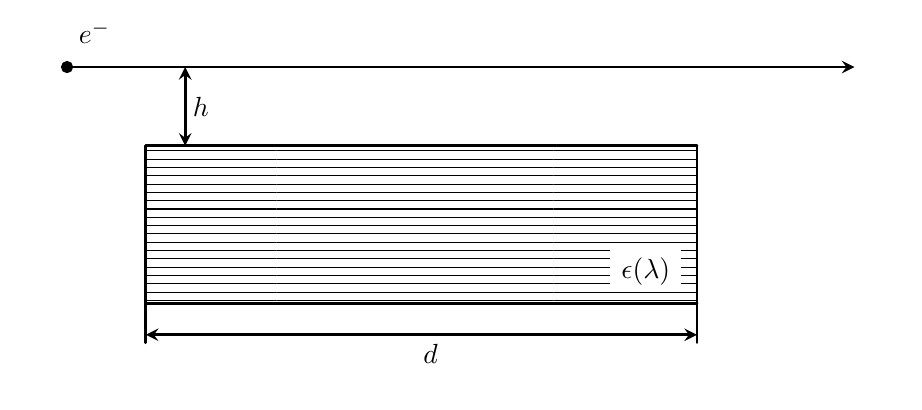
\begin{tikzpicture}[line cap=round,line join=round,>=stealth,x=1cm,y=1cm]

\clip(-0.5,-4) rectangle (10.5,0.5);

\fill[line width=1pt,fill=black,pattern=horizontal lines,pattern color=black] (1,-1) -- (8,-1) -- (8,-3) -- (1,-3) -- cycle;
\fill[line width=2pt,color=white,fill=white,fill opacity=1] (6.9,-2.3) -- (7.8,-2.3) -- (7.8,-2.8) -- (6.9,-2.8) -- cycle;

\draw [->,line width=1pt] (0,0) -- (10,0);
\draw [line width=1pt] (1,-1)-- (8,-1);
\draw [line width=1pt] (8,-1)-- (8,-3);
\draw [line width=1pt] (8,-3)-- (1,-3);
\draw [line width=1pt] (1,-3)-- (1,-1);
\draw [line width=1pt] (1,-3)-- (1,-3.5);
\draw [line width=1pt] (8,-3)-- (8,-3.5);

\draw [->,line width=1pt] (3.2,-3.4) -- (8,-3.4);
\draw [->,line width=1pt] (3.2,-3.4) -- (1,-3.4);
\draw (4.4,-3.4) node[anchor=north west] {$d$};

\draw [->,line width=1pt] (1.5,-0.5) -- (1.5,0);
\draw [->,line width=1pt] (1.5,-0.5) -- (1.5,-1);
\draw (1.7,-0.5) node[anchor=center] {$h$};

% \draw [line width=1pt,color=white] (7,-2.3)-- (7.8,-2.3);
% \draw [line width=1pt,color=white] (7.8,-2.3)-- (7.8,-2.8);
% \draw [line width=1pt,color=white] (7.8,-2.8)-- (7,-2.8);
% \draw [line width=1pt,color=white] (7,-2.8)-- (7,-2.3);
\draw (7.35,-2.6) node[anchor=center] {$\epsilon(\lambda)$};

\draw (0.025897872502580122,0.7) node[anchor=north west] {$e^-$};


\draw [fill=black] (0,0) circle (2pt);
\end{tikzpicture}
\caption{Schematic representation of a particle passing in proximity to a flat dielectric radiator.}
\label{fig:PCA_flat_radaitor}
\end{figure}


Although it is not possible to study analytically the radiation production in a target with complex shape, it is instructive to consider the emission for a flat dielectric radiator of finite length. Figure~\ref{fig:PCA_flat_radaitor} depicts a particle passing parallel to a flat dielectric radiator, with an impact parameter~$h$ and a radiator length $d$. The interaction of the particle field with the radiator will generate one forward and one backward DR front when the particle field encounters each perpendicular edge of the material. Additionally, as the particle travels along the radiator surface, the ChDR front will also form inside the target. The different components of energy lost by the particle due to the radiation were estimated using PCA~\cite{Shevelev:2014doa}.


The spectrum of emission for a single particle due to DR losses is given by~\cite{CERN-Report-II}:
\begin{equation}
\begin{aligned}
\left(\frac{dW}{d\lambda} \right)_\text{DR} = \, & \alpha \hbar c \sqrt{\frac{\gamma}{2 h}} \left( \frac{\epsilon(\lambda) -1 }{\left( \epsilon(\lambda) \mp 1  \right)^2}  \right)^2 \cdot \\ & \cdot \frac{1 - \text{cos}\left[ 2\pi d \left( \sqrt{\epsilon(\lambda) \mp 1} \right) /\lambda\right]}{\lambda^{3/2}} \, \text{exp}\left\{ -\frac{4\pi h}{\gamma \lambda} \right\}
\end{aligned}
\end{equation}
where $\alpha$~is the fine structure constant, $\hbar$~is the reduced Planck constant, $\gamma$~is the Lorentz factor, $\lambda$ is the wavelength and $d$~the dielectric length. In the $\pm$ terms, the  negative and positive signs describe the forward and backward DR, respectively. Similarly, the spectrum of emission of a single particle for ChDR losses is~\cite{CERN-Report-II}:
\begin{equation}\label{eq:chdr_loss}
\begin{aligned}
\left(\frac{dW}{d\lambda} \right)_\text{ChDR} = \,&   \frac{\alpha \hbar c}{2\pi \Theta_m} \frac{1}{\lambda\sqrt{\lambda B}} \frac{\sqrt{\epsilon\left(\lambda \right)-1}}{\epsilon\left(\lambda \right)} \, \text{erf} \left[ \sqrt{\frac{\pi B}{\lambda}} \phi_m \right] \cdot \\ & \cdot \left( \frac{A\Theta_m}{\lambda} \, \text{si}\left[\frac{A\Theta_m}{\lambda} \right]  + \text{cos}\left[\frac{A\Theta_m}{\lambda} \right] -1 \right) \, \text{exp}\left\{ -\frac{4\pi h}{\gamma \lambda} \right\}
\end{aligned}
\end{equation}
where $\Theta_m$ and $\phi_m$ are the polar and azimuthal angles describing the size of the Cherenkov cone, $\text{erf}(x)$ is the error function, $\text{si}(x)$ is the sine integral function~\cite{Brychkov:1251968}, and the $A$ and $B$ factors are 
$$A = 2\pi d \sqrt{\epsilon \left( \lambda \right) -1 }$$ 
$$B = 2\gamma h \left(\epsilon \left( \lambda \right) -1 \right)$$


The field of a particle bunch is the sum of the radiation of the individual particles~\cite{MOTZ}. The emitted radiation from a bunch of particles can be expressed as \cite{tesla_report}
\begin{equation}
I(\omega) = I_\text{SP}  \left(\omega\right) \,
\left( N + N \left( N -1 \right) \left| f \left(\omega\right) \right|^2 \right) \label{eq:coh-rad} 
\end{equation}
where $I_\text{SP}$ is the single-particle emission, $N$ is the number of particles in the bunch and $f(\omega)$ is the bunch form factor, i.e. the Fourier transform of the bunch longitudinal profile. For a bunch with a Gaussian longitudinal charge distribution emitting ChDR, $I_\text{SP}$ is expressed by (\ref{eq:chdr_loss}) and $f\left(\omega\right)$ is the Fourier transform of a Gaussian curve. Two radiation components can be identified in Equation~\ref{eq:coh-rad}. The first term is the incoherent part of the emission, which is proportional to the number of particles $N$. The second term is the coherent part of the emission, which is emitted at wavelengths longer than the bunch length and therefore with very small phase differences in the emissions by the individual particles. This determines a constructive interference of the emissions of the single particles, that enhances the produced radiation intensity as $N\left( N -1\right) \sim N^2$.

For illustration, figure~\ref{fig:PCA_h_scan} shows the spectrum of ChDR emission by a Polytetrafluoroethylene (PTFE or teflon)  radiator exposed to a 100~pC 2~ps-long (1~$\sigma$) electron bunch for varying impact parameters and radiator lengths.

In summary, the total emission from a dielectric target depends on two main components: the Diffraction Radiation generated at the target edges, and the Cherenkov Diffraction Radiation generated by the interaction of the beam field with the radiator surface. The former depends on the geometry, materials and impact parameter, while the latter also depends on the radiator area that is exposed to the beam field. 



\begin{figure}[!h]
\centering
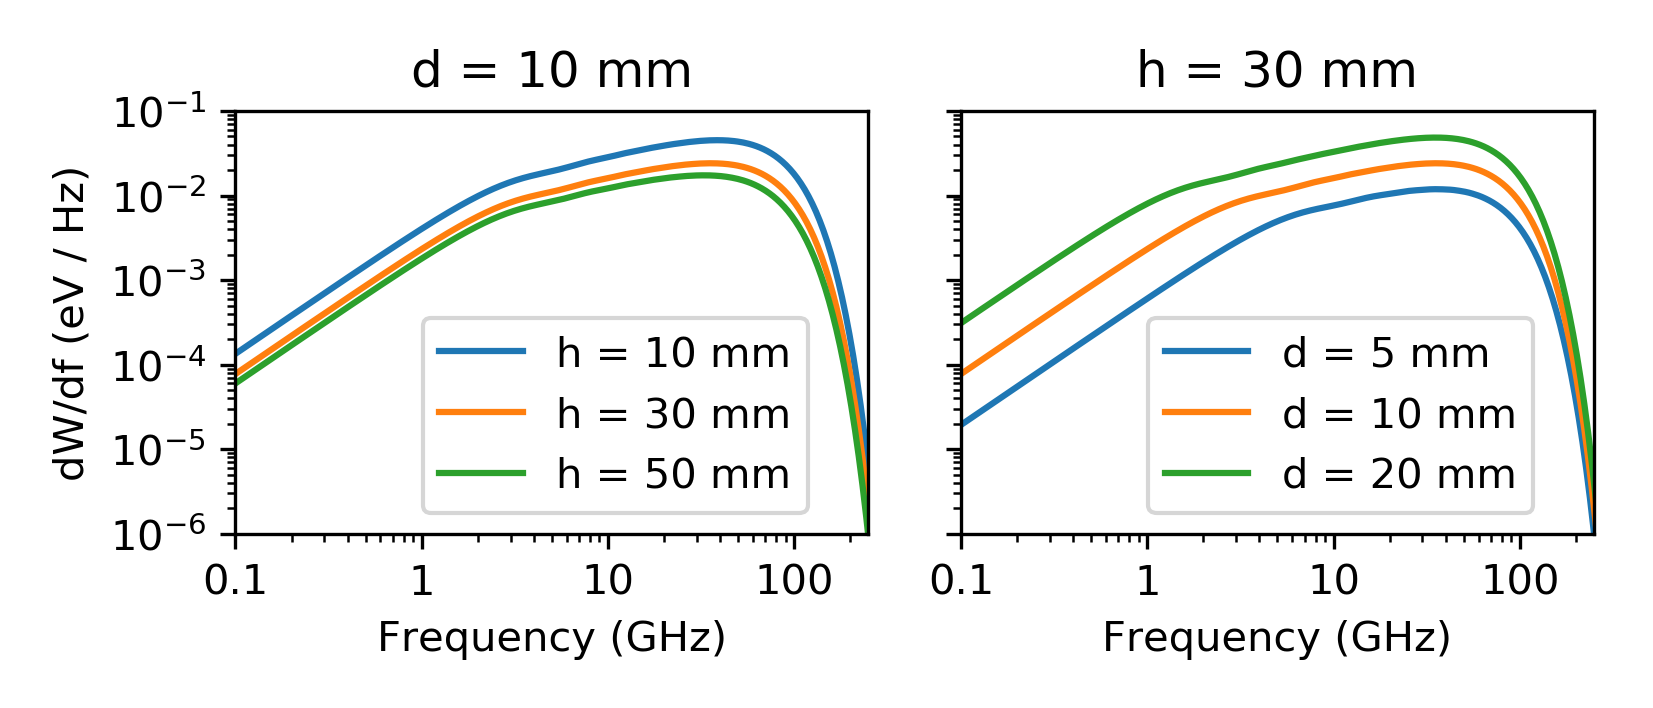
\includegraphics[scale=1, keepaspectratio]{pictures/PCA_h_d_scan}
\caption{Spectrum of ChDR emission for a 100~pC 2~ps-long electron beam passing in proximity to a PTFE flat target. On the left, the emission of a 10~mm long radiator was computed at various impact parameters. On the right, the impact parameter is kept constant at 30~mm and the length of the radiator is varied.}
\label{fig:PCA_h_scan}
\end{figure}






\section[A BPM prototype for in-air testing]{A BPM prototype for in-air testing}\label{sec:description}


A proof-of-principle beam position monitor prototype was designed at CERN. The goal of this design was to validate the use of ChDR for beam position monitoring while retaining the largest possible flexibility in the tests. For this reason, a simple and rather inexpensive design was realised for in-air testing. The test device was manufactured from a 26~cm-long aluminium tube. An internal beampipe diametre of 60~mm was chosen, matching the AWAKE common beamline dimensions. Figure~\ref{fig:Sketch_clear_bpm} illustrates the longitudinal section of the device. Four circular holes were drilled at $45^\circ$ angle and fitted with 18~mm-diameter PTFE inserts. The inner face of the dielectric inserts follows the beampipe curvature. The inserts are fixed to the main body with bolts.


\begin{figure}[!t]
\centering
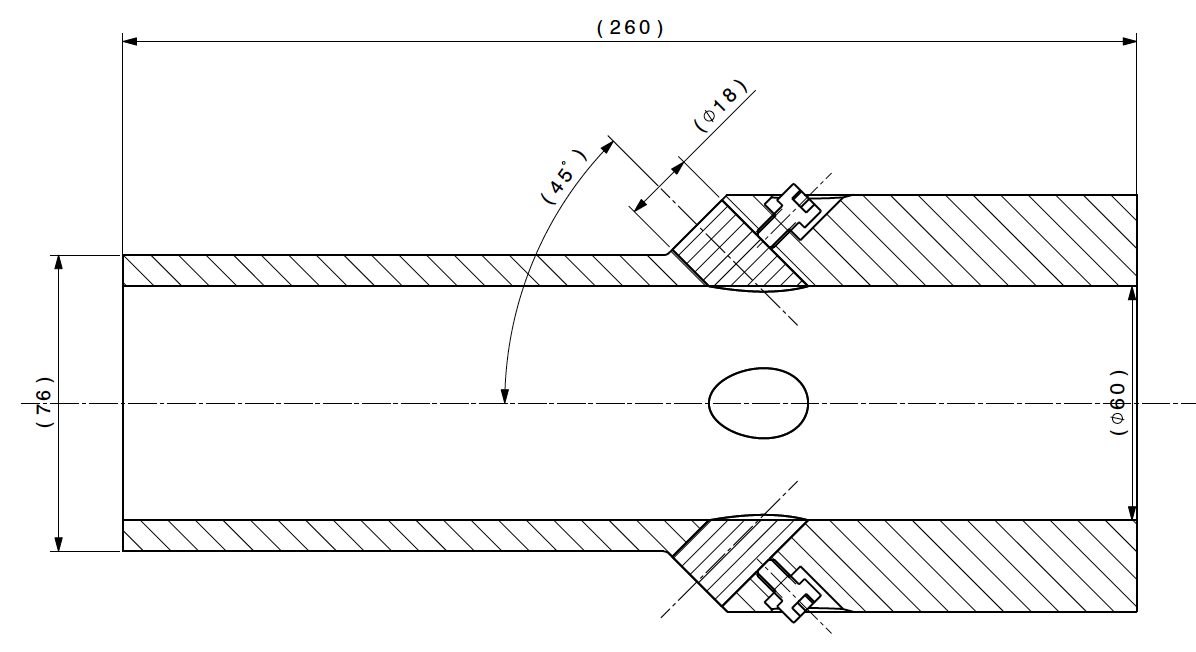
\includegraphics[width=14cm, keepaspectratio]{pictures/sketch_CLEAR}
\caption{A longitudinal section of the test device. The beam moves in the right-to-left direction. The two components oriented at $45^\circ$ and filled with the denser ruling are the PTFE inserts.}
\label{fig:Sketch_clear_bpm}
% \end{figure}


% \begin{figure}[!b]
\vspace{5mm}
\centering
% 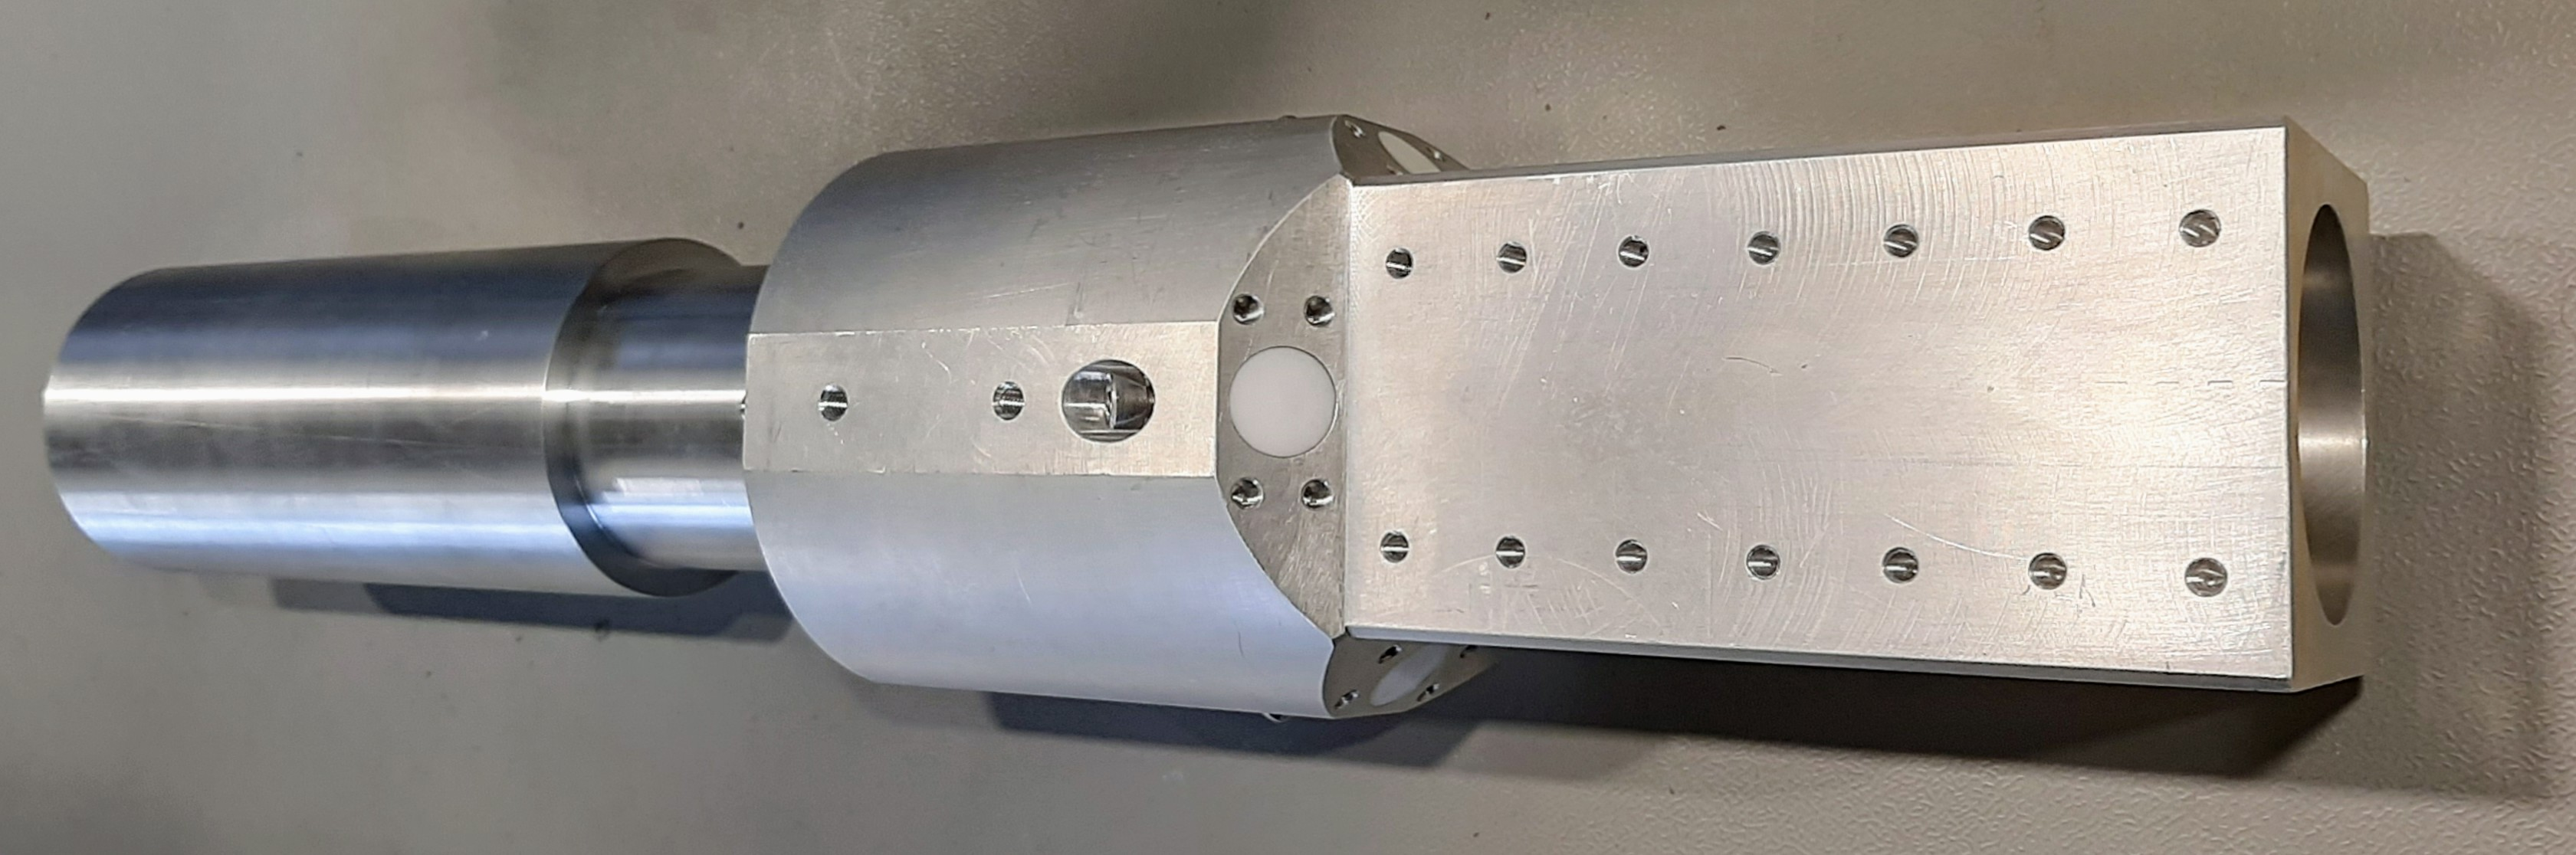
\includegraphics[width=13cm, keepaspectratio]{pictures/bpm+pipe}
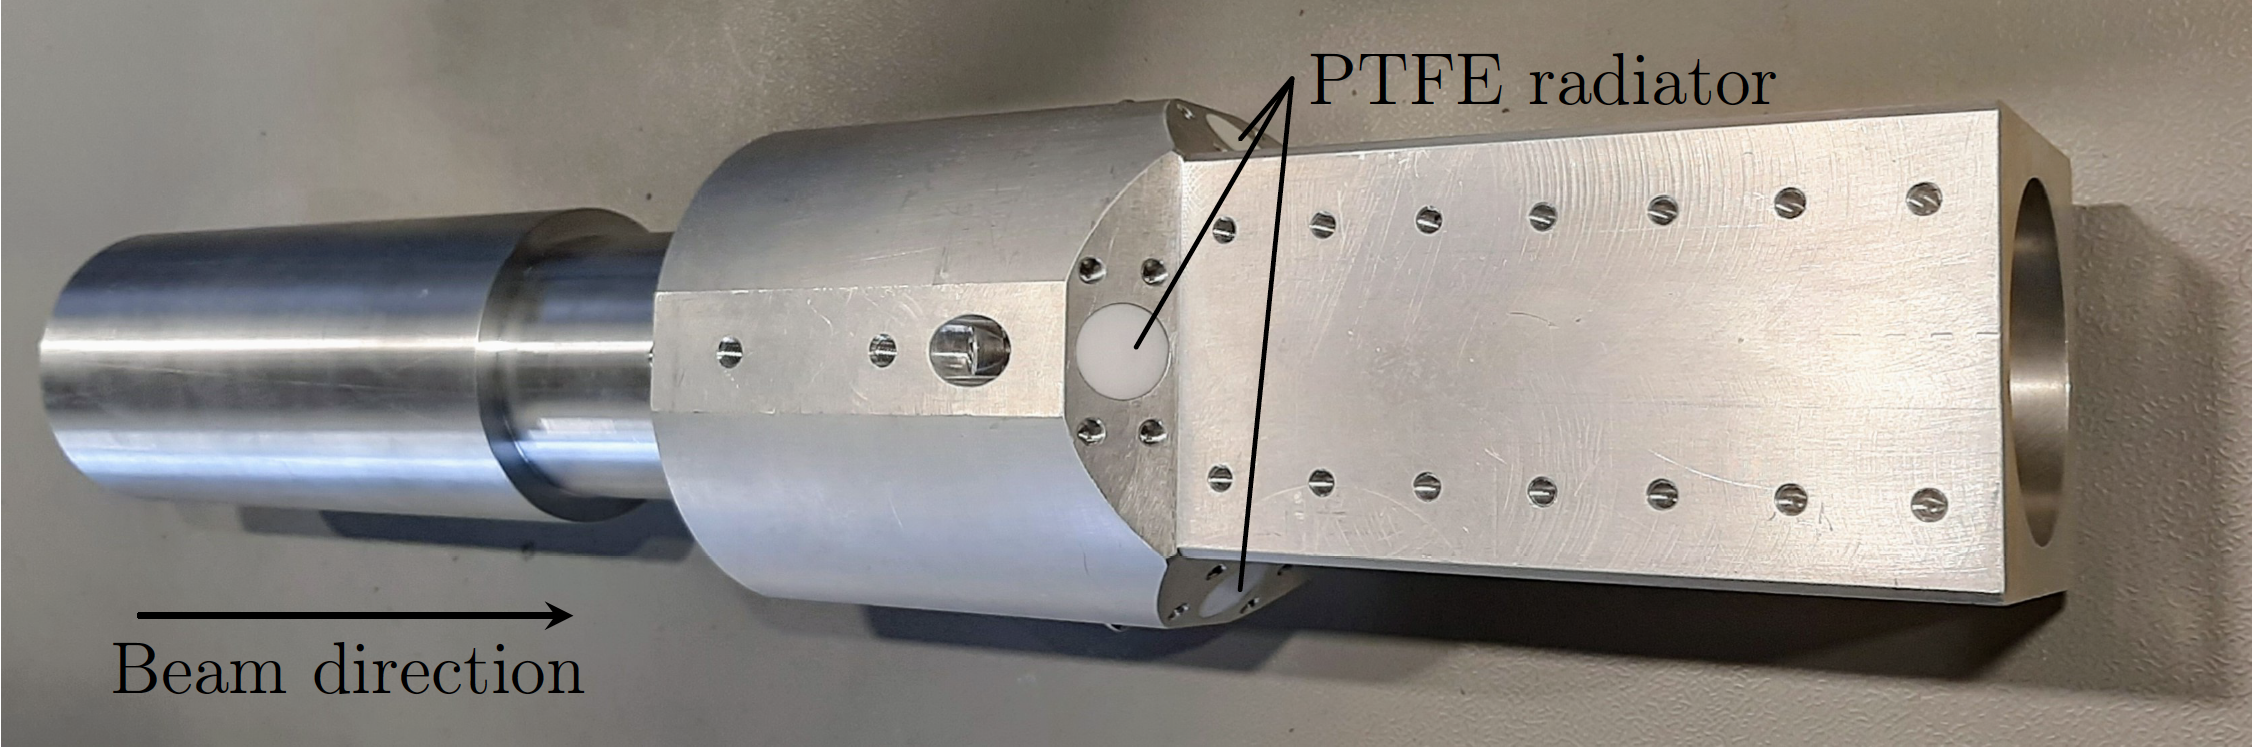
\includegraphics[width=13cm, keepaspectratio]{pictures/bpm+pipe+caption}
\caption{The test device with the extension tube installed. The beam direction is left-to-right. The white disks on the faces cut at $45^\circ$ are the radiator output surfaces. Above the radiator, the fixing bolt is visible. The part of the device downstream from the radiators has a square external shape and was fitted with threaded holes to support the detection system.}
\label{fig:clear_bpm_lab}
\end{figure}
% \vspace{2mm}
\begin{figure}[!h]

\subfigure[The four PTFE inserts seen from inside the beampipe. The four white disks are the radiators machined to be flush with the beampipe inner surface.]
  {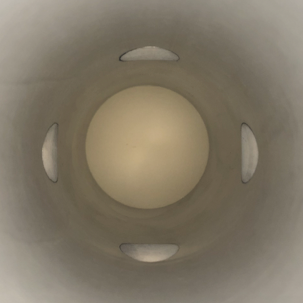
\includegraphics[width=6.5cm,keepaspectratio]{pictures/bpm_inside}}
\hspace{3mm}
\subfigure[The RF detectors installed on supports downstream of the radiators. The white disk on the metallic edge oriented at $45^\circ$ is the face of the radiator that emits the electromagnetic wave into air. The electric field is then coupled into the waveguide facing the radiator.]
  {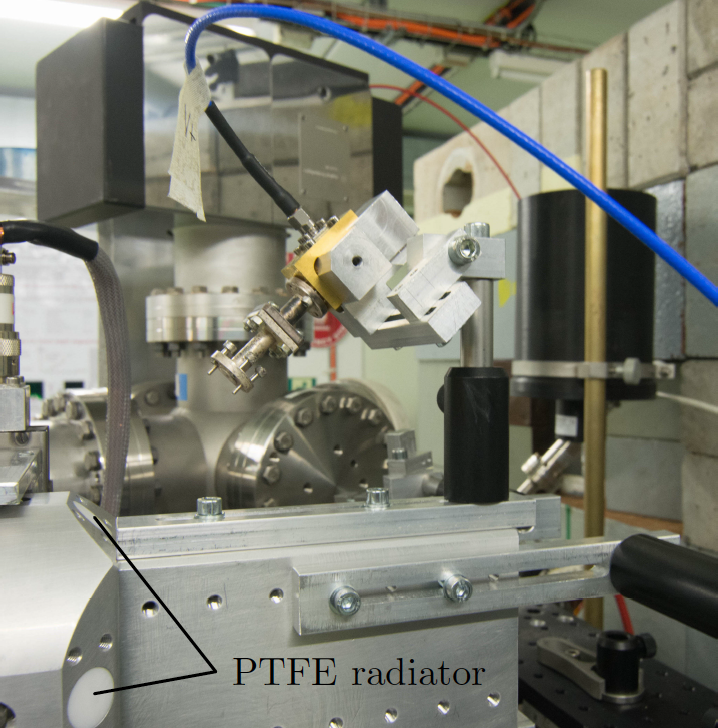
\includegraphics[width=6.5cm,keepaspectratio]{pictures/detail_diode_caption}}
\caption{The PTFE inserts and the RF detectors of the test device.}
\label{fig:bpm_details}

\end{figure}


The test device is depicted in Fig.~\ref{fig:clear_bpm_lab}. As the particle beam passes through the device, ChDR is generated at the radiator surface. It then propagates through the radiator and finally is emitted in air. Figure~\ref{fig:bpm_details}~(a) shows  the PTFE radiator surface trimmed inside the beampipe. The produced electromagnetic wave is then coupled to RF detectors. The downstream section of the test device features multiple tapped holes used to fix the RF detection system. Figure~\ref{fig:bpm_details}~(b) shows the RF detection system mounted on its support. Each detector is housed in a metal case that is clamped to a support pillar. Standard optical posts were used for this purpose. The support of the pillar can slide, adjusting the distance from the radiator. By means of this system, the distance and orientation of the detection system with respect to the radiator can be adjusted. The test device, and all the support part were designed and manufactured in-house.

To reduce electromagnetic disturbance due to geometric discontinuities, a metal extension tube with a matching internal diameter was fixed to the upstream end of the test device. The whole assembly was supported on an external bracket which could then be attached to a static or motorised support.

The electric field generated by the test device was measured using commercially available zero-bias\footnote{Zero-bias RF detectors are a class of RF detectors that does not require a bias voltage to operate.} RF detectors enclosed in a metal cases with a waveguide input and a coaxial output. The detection system is described in detail in Section~\ref{sec:setup}.








\section[Electromagnetic simulations]{Electromagnetic simulations}\label{sec:simulations}

A 3D model of the test device was created in CST Studio~2018 \cite{CST} for electromagnetic simulations. The test-device dimensions, shown in Fig.~\ref{fig:Sketch_clear_bpm}, are large compared to the sub-millimetre wavelengths generated by the short electron bunch. The initial attempts with uniform (or automatic) meshing of the model led to more than $2^{31}$ mesh cells, which cannot be simulated using the available resources, as it would require access to a multi-node computer cluster. Therefore, the model had to be simplified. An additional issue arose due to the large volume of air added outside the device in order to reliably reproduce the test conditions. 

Out of the multiple electromagnetic-field solvers available in CST, two were considered to simulate the test device: the wakefield solver and the Particle In Cell (PIC) solver. 

The wakefield solver uses the time-domain electromagnetic field of the moving bunch of charged particles. For the investigated problems, the simulated bunch had a Gaussian longitudinal profile and was relativistic. In this approach, the beam is only a source, and no feedback effect of the EM fields on the beam is considered. A big advantage of the wakefield solver is that the beam field is considered also at the boundaries so the beam field enters the simulation domain smoothly with the correct shape \cite{CST:pc}. 

The Particle In Cell (PIC) solver approximates the beam as a group of macroparticles, each of them carrying a given charge and with its own coordinates in the bunch. The macroparticles are treated independently and interact with themselves and the EM fields in their environment. Accordingly, PIC solvers are extensively used in plasma physics \cite{OSIRIS} and in beam dynamics studies with space charge \cite{pyORBIT}. Such an analysis allows the user to define any beam-charge distribution, provided that the number of macroparticles is sufficiently high. Further advantages include the possible exploitation of GPU computing and low noise in specific simulation conditions \cite{PIC:reduction_noise}. An important drawback of the PIC solver is that the beam fields are distorted at the simulation domain boundaries, and some space must be allowed for the field to develop in a realistic way. Figure~\ref{fig:pic_vs_wak} compares the beam field computed by the PIC and wakefield solvers. 

Due to the large size of the simulation domain, it would be impractical (if not impossible) to use the PIC solver, as it requires an additional volume for the beam field to develop properly. Therefore, the wakefield solver was selected to simulate the test device after preliminary investigations at low resolution. Nevertheless, the model had to be simplified to be simulated with reasonable time and computing power. Two approaches were investigated independently: approximating the problem with a thin slice and appropriate boundary conditions, and applying custom meshing to reduce the computing power required to simulate a full test device with a single radiator.


\begin{figure}[!t]
\centering
\subfigure[Bunch electric field in a wakefield simulation.]{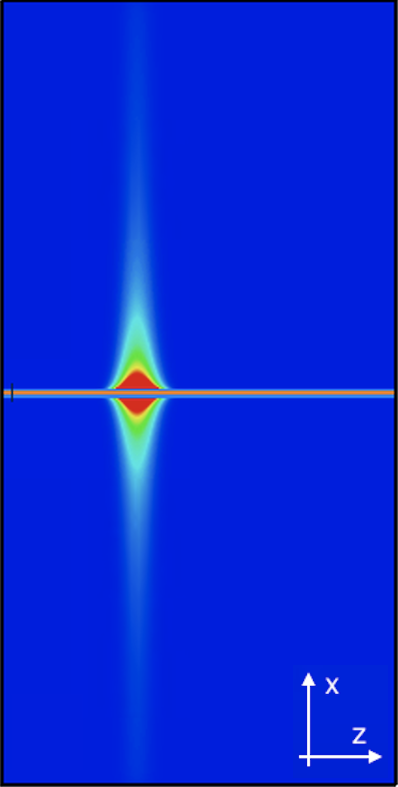
\includegraphics[width=2.8cm, height=5cm]{pictures/WAK_entrance}}
\hspace{2mm}
\subfigure[Bunch electric field in a PIC simulation.]{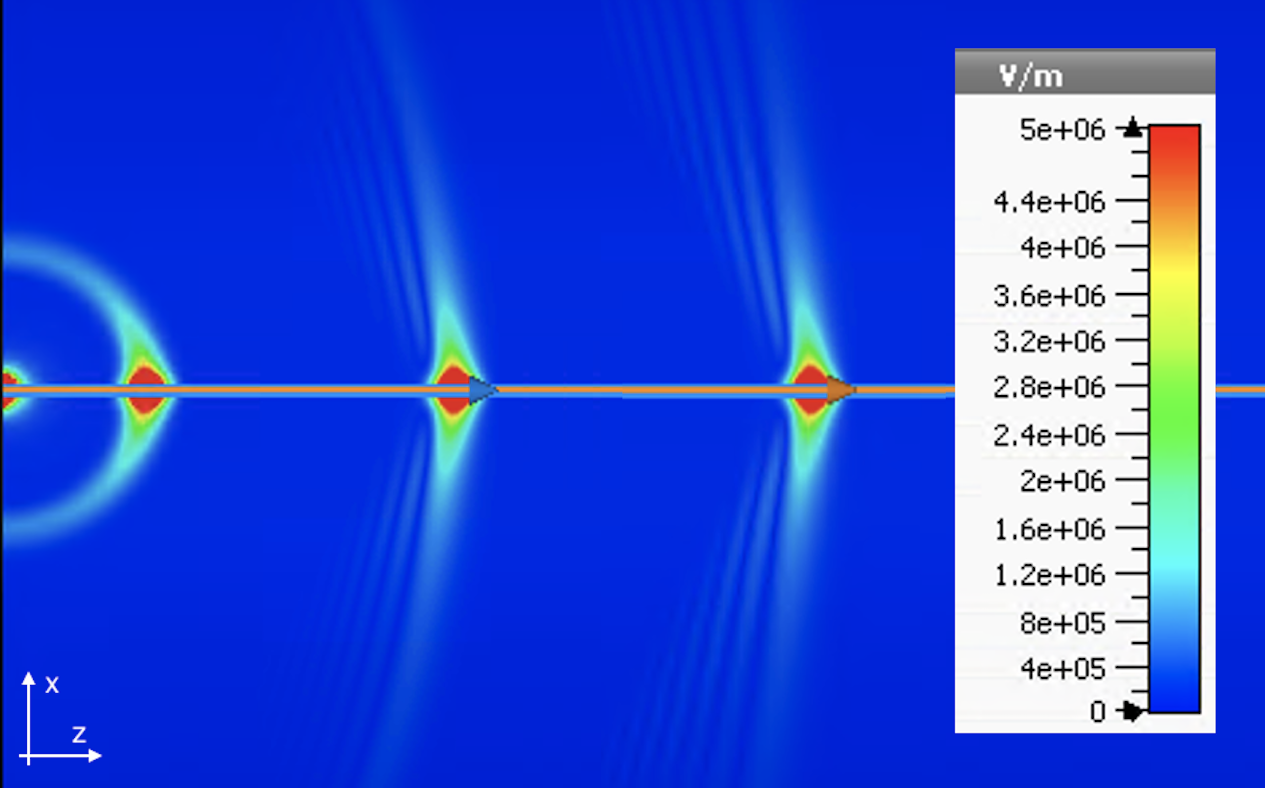
\includegraphics[width=9cm, height=5cm]{pictures/PIC_collage}}
% \subfigure[Bunch electric field in a wakefield simulation.]{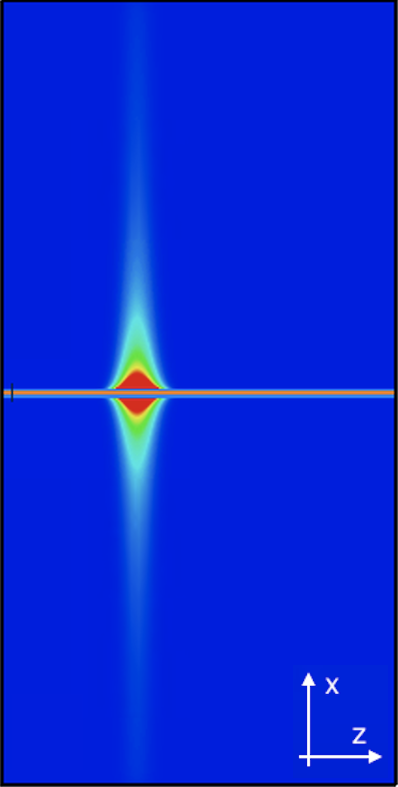
\includegraphics[height=5cm, keepaspectratio]{pictures/WAK_entrance}}
% \hspace{2mm}
% \subfigure[Bunch electric field in a PIC simulation.]{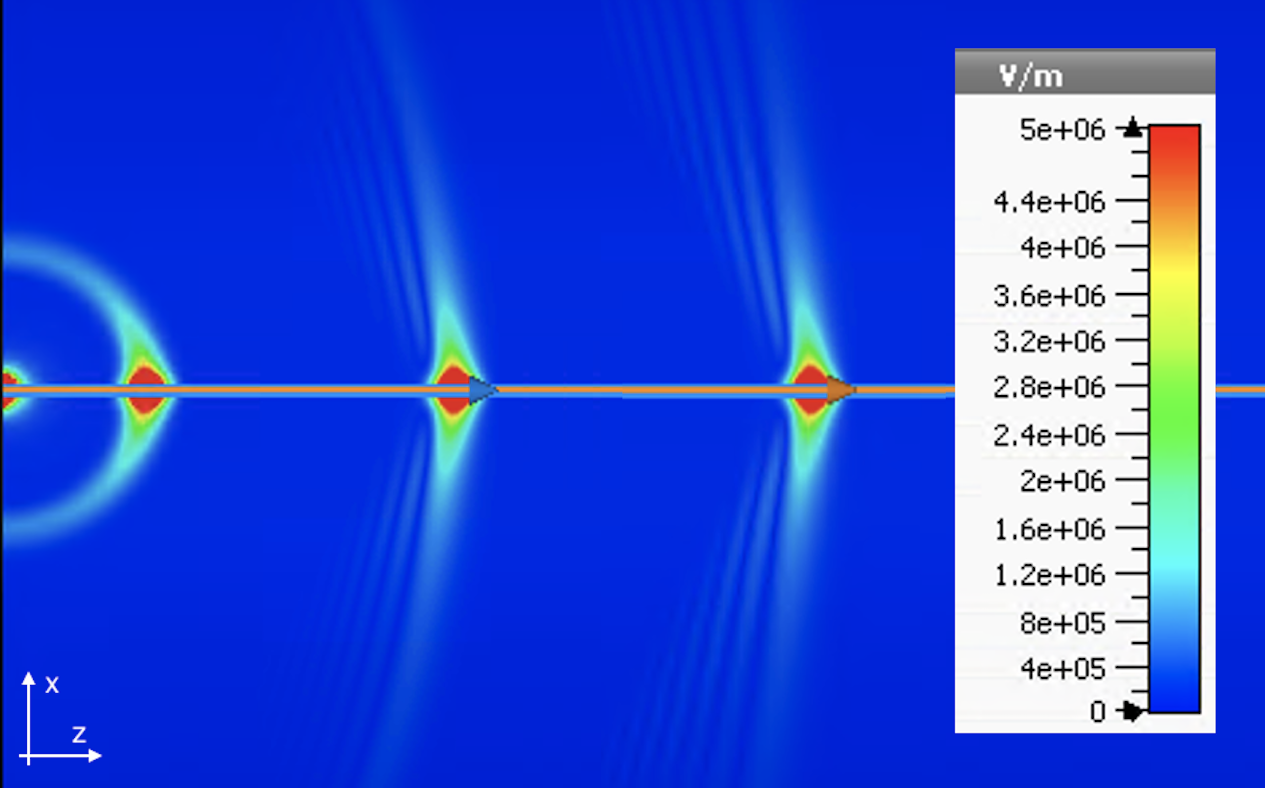
\includegraphics[height=5cm, keepaspectratio]{pictures/PIC_collage}}



\caption{Comparison of the beam electric field in vacuum close to the edge of the simulation domain for (a) the wakefield solver and (b) the PIC solver. The beam propagates left to right and the absolute value of the electric field is plotted. An electron bunch of 100~pC charge and 1~ps length is shown. In the wakefield simulation (a) the beam enters the simulation domain smoothly and the electric field is realistic already at the simulation domain boundary. The displayed frame shows the field density 20~ps into the simulation. Conversely, for the PIC simulation (b), there is some necessary time for the field to assume a realistic distribution. Picture (b) shows the field expansion process for the bunch at 2, 20, 100 and 200~ps into the simulation. A uniform meshing is used, assuring 100~GHz simulation bandwidth with 20 mesh cells per wavelength. The disturbance trailing the beam field in (b) is caused by the noise in the simulation, and can be controlled by decreasing the mesh cell size. The colour bar for the field intensity is valid for both plots.}
\label{fig:pic_vs_wak}
\end{figure}




\subsection[Simulation of a slice]{Simulation of a slice}\label{sec:slice_model}

\begin{figure}[!b]
\centering
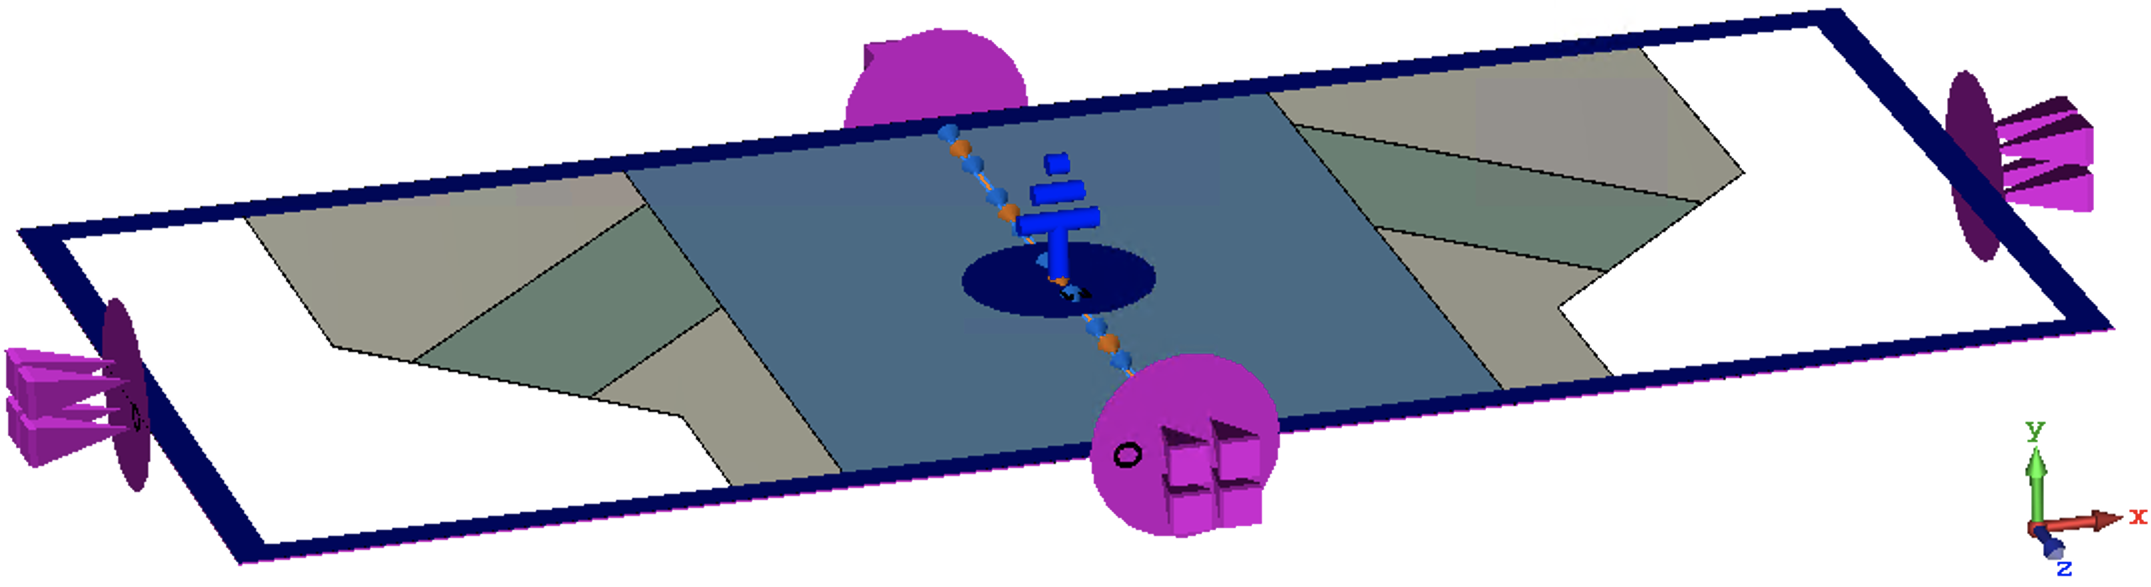
\includegraphics[width=14cm, keepaspectratio]{pictures/slice_boundary}
\vspace{1mm}
\caption{Boundary conditions of the slice model. The blue ground symbol represents the magnetic boundary condition (${\text{H}_\text{t}=0}$), which is applied at both edges of the simulation domain in the y direction. The violet symbol with the four pyramids represents the open boundary condition, used in all the other boundaries.}\label{fig:slice_boundaries}

\vspace{3mm}

\subfigure[t = 80 ps]{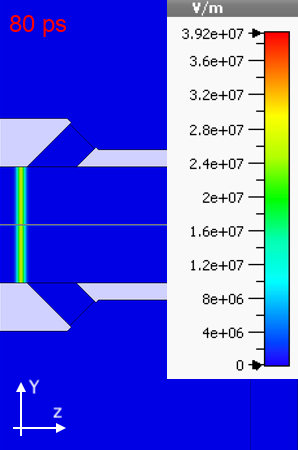
\includegraphics[width=3.55cm, keepaspectratio]{pictures/frame0}}
\hspace{1mm}
\subfigure[t = 160 ps]{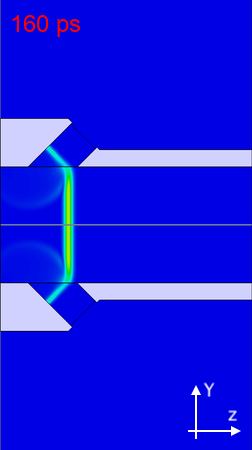
\includegraphics[width=3cm, keepaspectratio]{pictures/frame1}}
\hspace{1mm}
\subfigure[t = 200 ps]{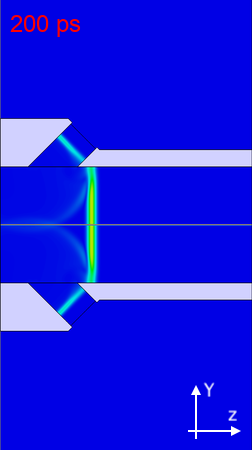
\includegraphics[width=3cm, keepaspectratio]{pictures/frame2}}
\hspace{1mm}
\subfigure[t = 400 ps]{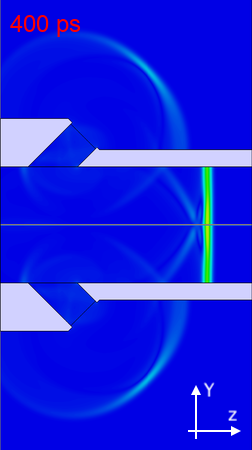
\includegraphics[width=3cm, keepaspectratio]{pictures/frame4}}
\caption{Electric field in the slice model at different time steps. In (a) the beam is propagating in the beampipe and has not yet interacted with the radiator. In (b) the beam is interacting with the radiator, producing the ChDR front that propagates at $45^\circ$ inside the radiator. Furthermore, the DR produced by the interaction with the upstream radiator edge is visible inside the beampipe with a circular wave-front. In (c) the propagation continues after the beam passed the radiator and the ChDR front advances. After exiting the radiator (d), the field expands in vacuum as a circular wave. The formation of additional circular DR fronts due to the interaction with the radiator edges visible in (b), (c) and (d) is described later for the 3D simulation. The simulation parameters are: a simulation bandwidth of 50~GHz, 20~mesh cells per wavelength, 100~pC and 5~ps long electron beam.}
\label{fig:slice_forward propagation}
\end{figure}


As the first attempt to simplify the model and reduce the simulation size, the test device was cut longitudinally into a quasi-2D model. In the past, researchers at other institutes used the 2D electromagnetic simulation code MAGIC~\cite{MAGIC} for simpler designs. However, MAGIC was not available for simulations of the test device and CST Studio does not offer 2D solvers. A similar approximation was nonetheless achieved by applying appropriate boundary conditions to a thin slice of the full model. A longitudinal slice of the test device was made just a few mesh cells thick. Open boundary conditions were used on four sides, but in the cutting plane where magnetic boundary conditions (${\text{H}_\text{t}=0}$) were used (see Fig.~\ref{fig:slice_boundaries}). Perfect vacuum was used as a background material. Despite being an approximation of the full model, such an approach gave insight into the internal propagation of the electromagnetic fields. However, in the thin slice model the DR generation is affected by the approximated geometry of the material edges. Fig~\ref{fig:slice_forward propagation} shows the formation of the ChDR front at the beam passage, and the propagation of the electromagnetic fields that follow. The importance of having a quickly running model to assess the internal reflections will be manifest in Section~\ref{sec:directivity} where the effect of the back-propagation of the beam through the device is shown. 








\subsection[3D Simulation of a single radiator]{3D Simulation of a single radiator}\label{sec:single_electrode}

Although the simulation of a slice shows how the electromagnetic radiation propagates inside the device, a more quantitative 3D simulation is beneficial. The DR that is generated depends on the geometry of material discontinuities and edges that are present, in this case, in the beampipe. These cannot be reliably modelled with a thin slice and a full 3D simulation is necessary.

\begin{figure}[!b]
\centering
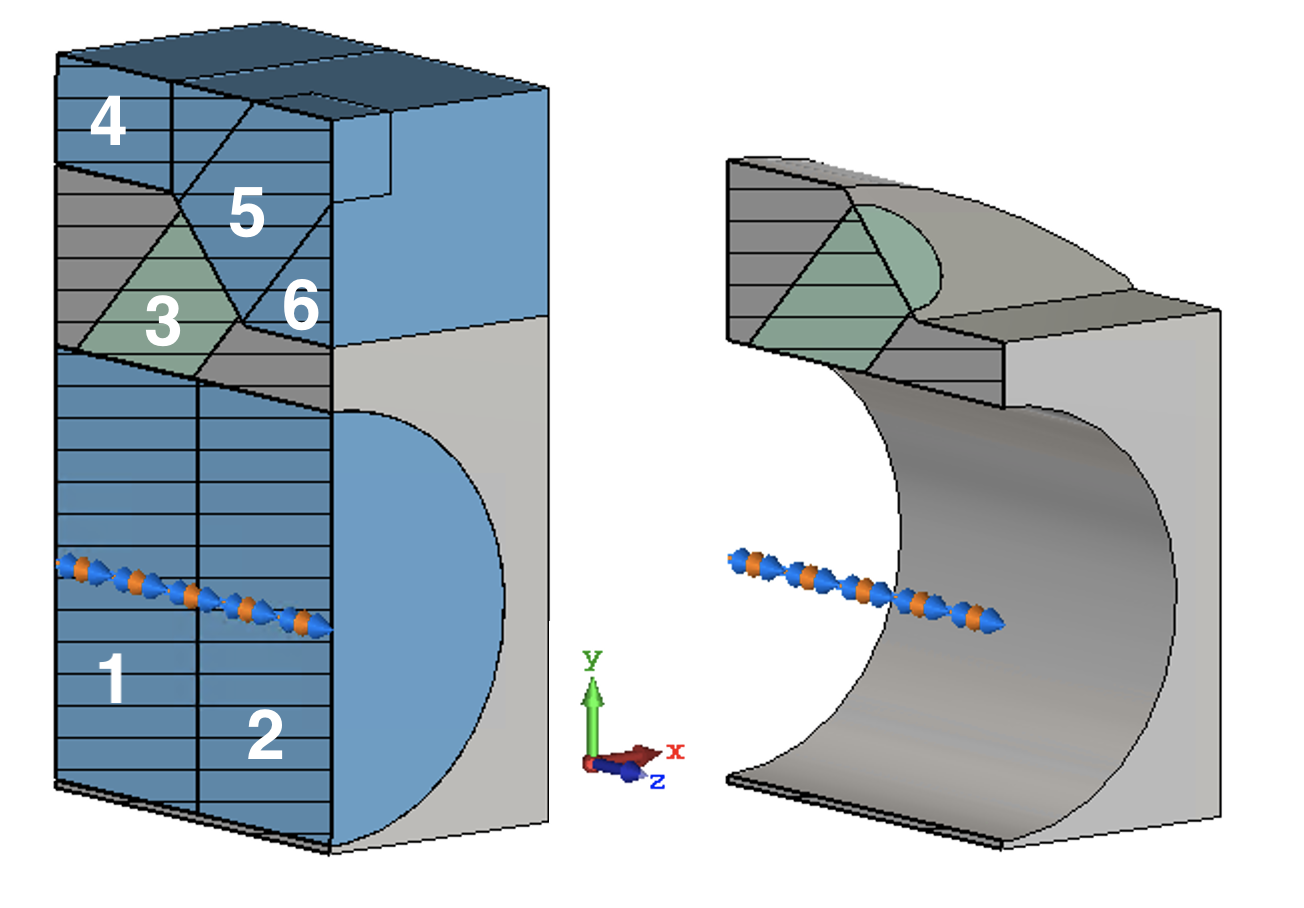
\includegraphics[scale=.6, keepaspectratio]{pictures/cut_simulation_both}
\caption{Longitudinal section of the 3D model used for the electromagnetic simulations. On the left the model is displayed including the vacuum parts and indicating the different meshing regions, on the right the vacuum volumes are hidden. Light blue volumes are made of vacuum, light green volume is the PTFE radiator, and volumes in grey are metal. The orange and blue arrows indicate the propagation path and direction of the beam.}
\label{fig:simulation_zones}
\end{figure}

For 3D simulations, the model was divided into six areas, shown in Fig.~\ref{fig:simulation_zones}. To minimise the simulation time, each area was meshed with a different resolution. In the figure, the beam propagates left-to-right along the path indicated by the orange and blue arrows. Inside the beampipe, the beam propagates in vacuum through regions~1 and~2. Region~1 contains the interface with the radiator. When the beam leaves region~1, it stops contributing to the production of electromagnetic waves in the radiator, and therefore region~2 is excluded from the simulation to save computing resources. The produced ChDR and DR propagate through the dielectric radiator, marked with 3. At the radiator exit face, the radiation starts to propagate in free space. As the radiation is produced at the Cherenkov angle, at which also the radiator is installed, the radiation exits along the normal to the radiator face. Therefore, region 5 is the most interesting as it is where the forward emitted radiation is present. Region 6 is meshed with a coarser mesh as the fields generated there are not so interesting, saving substantial computing resources. The metal volume is treated with the same mesh resolution as region 6. To save additional computing resources, region 4 is also excluded from the simulation. 

Regions 1, 3 and 5 are vital to understand the operation of the test device, while the other regions can be ignored or simulated with lower resolution. To achieve this, different mesh groups are defined manually, with the parameters reported in Table~\ref{tab:meshing}. At the interface between regions with different mesh size, the finest meshing is extended to the adjacent region for 1~mm. 

Such a meshing technique led to a tenfold reduction of the number of mesh cells compared with the same 3D model with uniform meshing and 20 cells per wavelength. Usually, simulations with the optimised mesh completed in less than two days on the CERN computing cluster. 





\begin{table}[!b]
  \centering
    \begin{tabular}{l c c c c}
    \toprule
    Mesh group &  Cells/$\lambda$ & Cell size (mm) & Regions on Fig.~\ref{fig:simulation_zones}\\
    \midrule
    High resolution     & 20    & 0.15  & 1, 3, 5\\
    Low resolution      & 3    & 1  & 6\\
    Metal               & 3    & 1  & -\\
    Do not simulate     & 0    & -  & 2, 4\\
    \bottomrule
    \end{tabular}
  \caption{Parameters of the different meshing regions used in the simulations. The calculations are performed for a simulation bandwidth of 100 GHz which corresponds to a wavelength of 3~mm.} \label{tab:meshing}
\end{table}


An additional complication of large volume and large bandwidth simulations is the size of the output, which is of the order of 25~GB and 15~thousand files for the discussed model. Most of the space is used to save the field monitor outputs. Due to the size of the simulation, the field values can be recorded only by probing the field in a point or on a plane, but not in the whole simulated volume. Given the output size, transferring the simulation results from the computing cluster to the local computer is  a complex operation and can require up to half a day, which has to be added to the computing time.

\begin{figure}[!b]
\centering
\subfigure[t$=90$ ps]{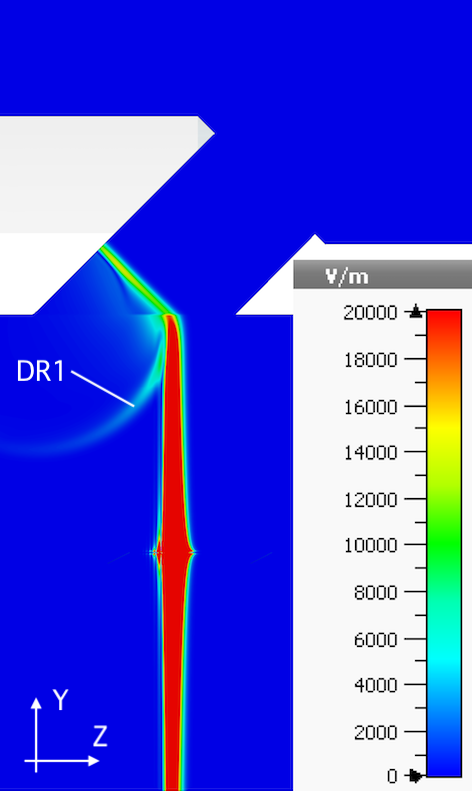
\includegraphics[width=4cm, height=6.8cm]{pictures/90ps}}
\hspace{2mm}
\subfigure[t$=140$ ps]{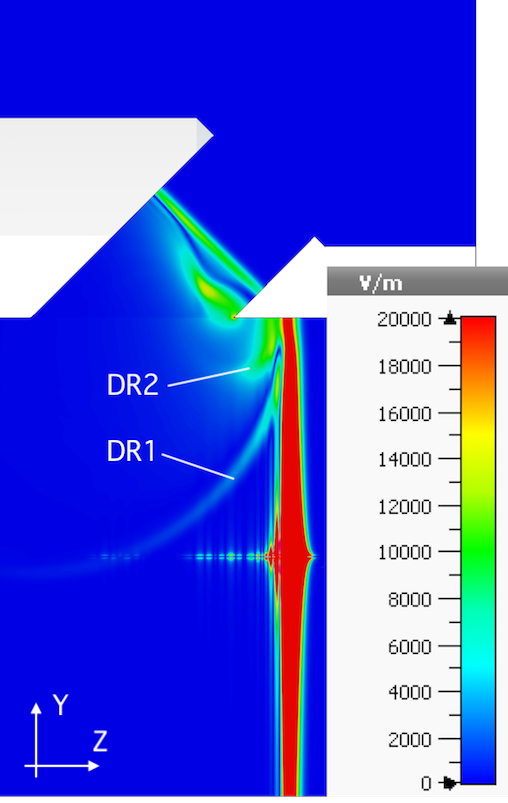
\includegraphics[width=4.3cm, height=6.8cm]{pictures/140ps}}
\hspace{2mm}
\subfigure[t$=220$ ps]{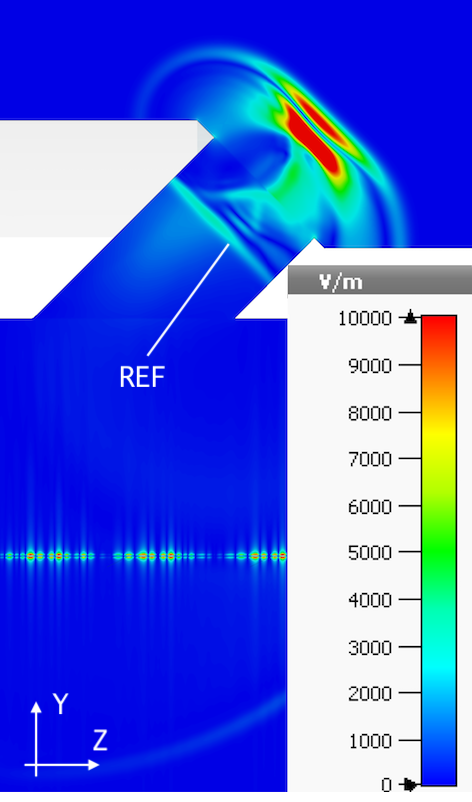
\includegraphics[width=4cm, height=6.8cm]{pictures/230ps}}
\caption{3D simulation of the electric field produced by the beam passing next to a PTFE radiator with the same geometry as the one used for the tests at CLEAR. The grey and white areas represent the metal pipe. The ChDR and DR front formations are visible and are described in detail in the text.}
\label{fig:field_CLEAR_simulation}
\end{figure}

The result of a simulation for a 2~ps long, 100~pC electron beam propagating through the test device described in Section~\ref{sec:description} is presented in Fig.~\ref{fig:field_CLEAR_simulation}. The picture shows the absolute value of the electric field 90, 140 and 220~ps into the simulation. The results offer valuable insights into the electromagnetic radiation production mechanics. Figure~\ref{fig:field_CLEAR_simulation} (a) shows the beam as it passes next to the radiator. The ChDR front propagating at the Cherenkov angle inside the radiator is clearly visible. An additional spherical front is visible inside the beam pipe following the direct field of the bunch (marked as DR1). This is the DR front generated at the discontinuity due to the upstream edge of the radiator. In (b) the beam has passed the radiator. A second front of DR both in the beampipe and in the radiator is visible, provoked by the interaction with the downstream radiator edge (indicated as DR2). Looking forward in time in (c), the electromagnetic wave has left the radiator. The forward front being ChDR, while the trailing wavefront is the DR from the interactions with the radiator edges. Looking more carefully inside the radiator, there is a less intense front of radiation visible that was reflected back inside (indicated as REF). This is a part of the DR front, that traveled inside the radiator at some angle to the radiator output surface normal. On the other hand, the ChDR is completely emitted as it travels perpendicularly to the output surface. Please note that the field intensity scale of (c) had to be enhanced to visualise the reflected field.











\subsection[Position sensitivity]{Position sensitivity}\label{sec:position_sensitivity}

The absolute value of the electric field is considered as
\begin{equation}
E_\text{abs} = \sqrt{ E^2_\text{x} + E^2_\text{y} + E^2_\text{z} }
\end{equation}
where the different components of the field are calculated for each point in space and time. 

To estimate the response of the test device to beam-position variations, i.e. its sensitivity, the electric field is sampled in vacuum 10~mm above the centre of the radiator exit surface. The field probe position is shown in Fig.~\ref{fig:sim_t_scan}~(a). A number of different beam positions are simulated. Figure~\ref{fig:sim_t_scan} shows the absolute value of the electric field simulated in the time domain for three beam positions. The two peaks visible correspond to the two emission fronts of ChDR and DR that are clearly visible in Fig.~\ref{fig:field_CLEAR_simulation}~(c). 





\begin{figure}[!t]
\centering
\subfigure[Simulation model.]{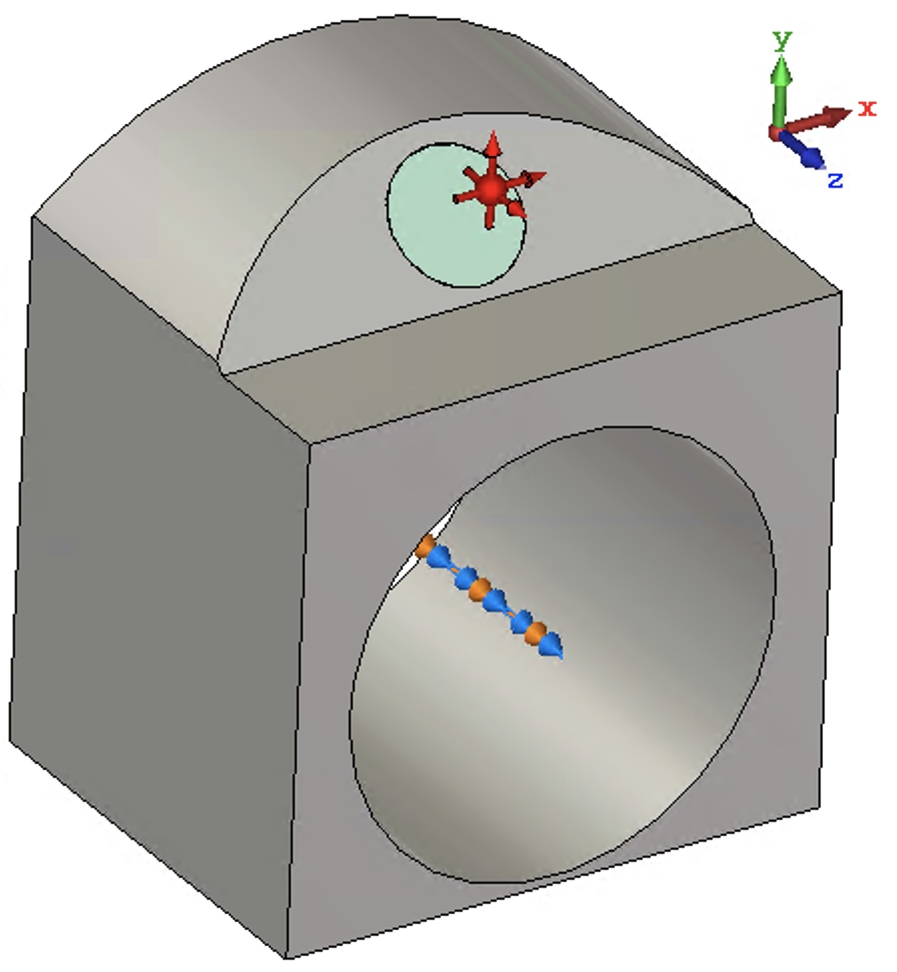
\includegraphics[width=53mm, keepaspectratio]{pictures/Model+probe}}
\hspace{1mm}
\subfigure[Absolute value of the electric field at the probe position. ]{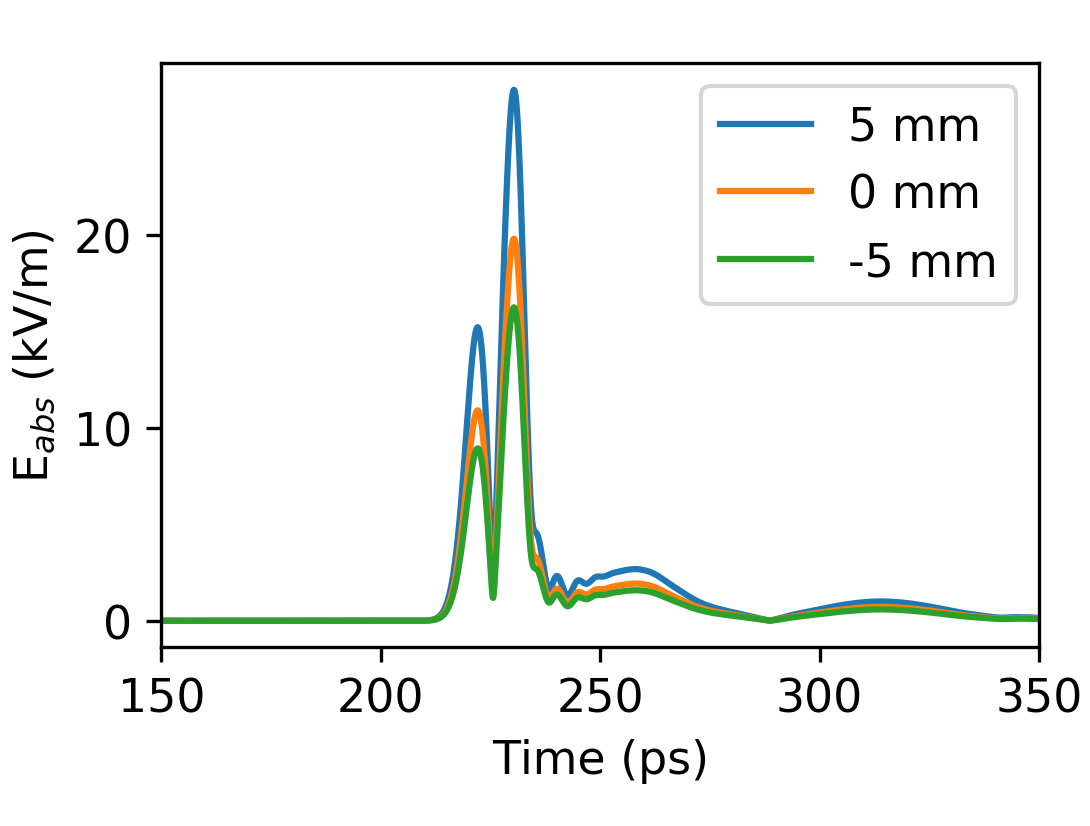
\includegraphics[scale=0.9, keepaspectratio]{pictures/sim_t_response.png}}
\caption{On the left, the simulated 3D model is shown, including the probe point of the electric field (in red). On the right, the absolute value of the electric field at the probe point is shown for three different beam positions.  Zero is the beampipe centre and the positive positions correspond to the beam getting closer to the radiator. The field is sampled in a single point, 10~mm above the centre of the radiator output surface.}\label{fig:sim_t_scan}
\end{figure}

The beam position was swept over a 30~mm range around the centre of the beampipe. The resulting electric field was considered over a 100~ps-wide window, and the RMS of the windowed signal was calculated. The $\Delta/\Sigma$ quantity was then computed from the RMS values. The opposite electrode was not simulated due to the limited computing resources, but its signal could be deduced from the response of the simulated electrode assuming symmetry. Figure~\ref{fig:sim_delta_sigma} shows the RMS electric field at the observation point from the simulated dielectric radiator and from the the opposite radiator (deduced from the geometry). The squared electric field was then used to compute the $\Delta/\Sigma$ as a function of the beam position. The device response exhibits a linear behaviour near the beampipe centre, and becomes non-linear for larger displacements. A linear fit for beam displacements of $\pm 3$~mm from the beampipe centre was carried out, resulting in a sensitivity of $1.3\times10^{-1} \text{ mm}^{-1}$.

\begin{figure}[!h]
\centering
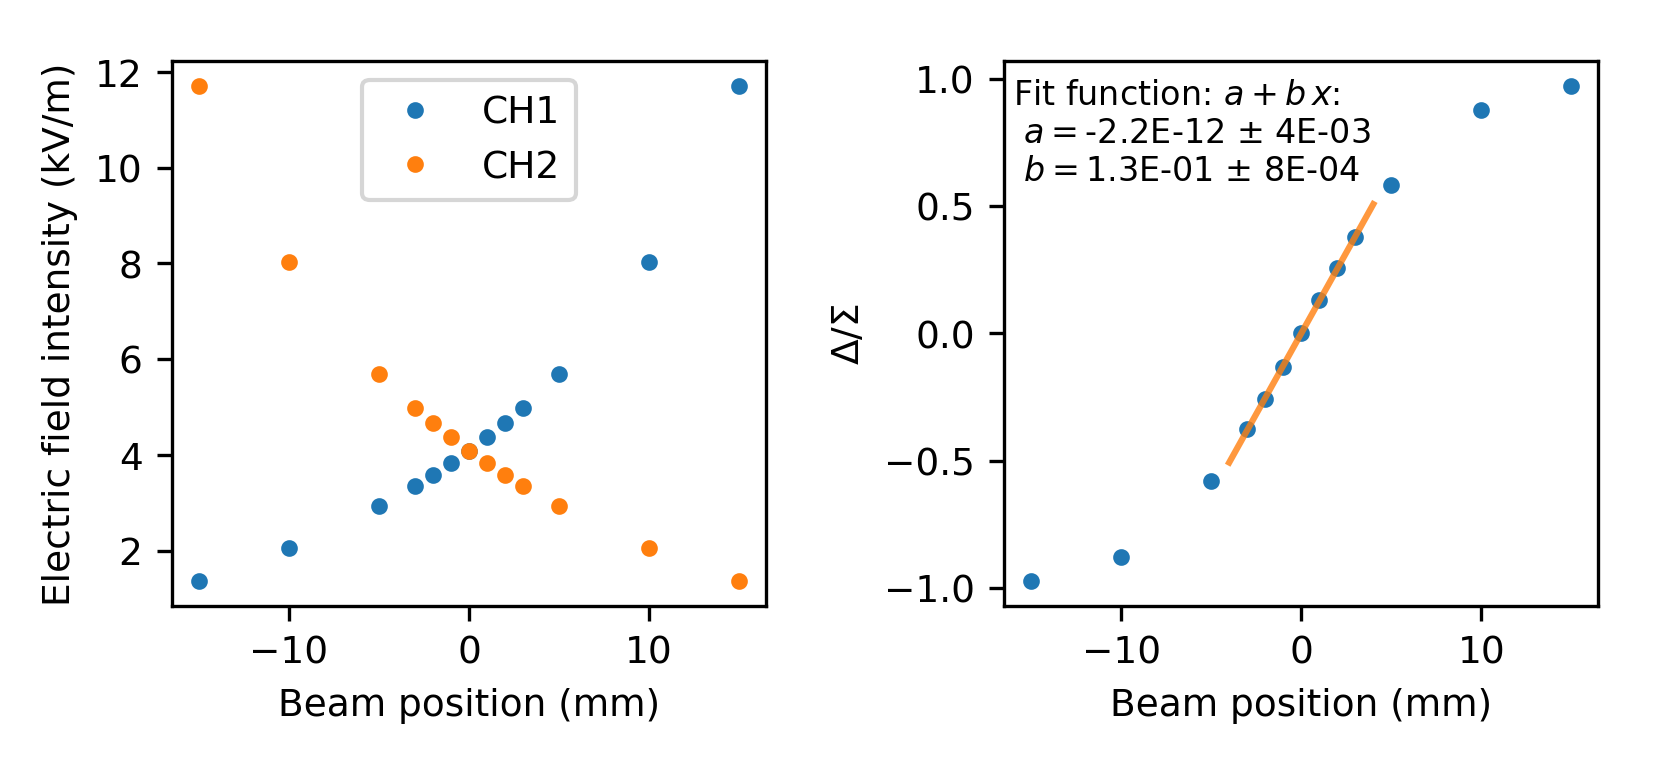
\includegraphics[scale=1, keepaspectratio]{pictures/sim_delta_sigma_both.png}
\caption{On the left, the RMS electric field emitted from the radiator measured at the test point shown in Fig.~\ref{fig:sim_t_scan}~(a). The signal from the second radiator is deduced by geometry. On the right, the  $\Delta/\Sigma$ quantity calculated from the simulation results for a beam displacement of $\pm15\text{ mm}$. The linear fit in the region of $\pm3\text{ mm}$ displacement is also reported.}\label{fig:sim_delta_sigma}

\end{figure}




\subsection[Improvements to the simulation capabilities]{Improvements to the simulation capabilities}

Two significant limitations of the CST wakefield solver were identified during the simulation work. First, the solver can only simulate particle bunches with a Gaussian longitudinal charge distribution. Secondly, waveguide ports, used to observe the generated electromagnetic waves, must be parallel to one of the simulation domain boundary planes. Therefore, they cannot be used to evaluate the overall field exiting from the radiator surface as it is not parallel to one of the axes. Solutions for both of these problems were studied and are described below. 



\subsubsection{A method to evaluate non-Gaussian bunches}

Even though the CST wakefield solver uses only bunches with a Gaussian longitudinal charge distribution, the model's transfer function can be calculated using signal-processing theory. Let us consider the simulation of a complex model like the one described in Section~\ref{sec:single_electrode}. The simulation can be seen as a system that transforms the time-varying beam current into an electromagnetic field that is probed in a point of space at a given time. The system in question is linear, as the superposition principle is valid, and it is also time-invariant, as the response does not change if the stimulus is applied with a delay. Therefore, the simulated model can be treated as a Linear Time-Invariant (LTI) system. 

In an LTI system, the output signal in the time domain is a convolution of the system's impulse response with the input signal, and the convolution is defined as 
\begin{equation}
h(t)\ast I(t) = \int_{-\infty}^\infty  h(t-\tau) I(t) d\tau
\end{equation}
where $h(t)$ is the system's impulse response and $I(t)$ is the input signal. 
In the frequency domain, the convolution simplifies to a product of the transfer function $H(f)$ and the input signal spectrum. A flowchart of this process is shown in Fig.~\ref{fig:LTI_system}. The frequency domain representation of a continuous time-varying signal is usually obtained using the Fourier transform. For the beam current and the probe field signal this operation is automatically provided by CST.



\begin{figure}[!t]
\centering
\begin{tikzpicture}[line cap=round,line join=round,>=triangle 45,x=1cm,y=1cm]
\clip(-6,-4) rectangle (8, 2);

\draw [line width=1pt] (-2,1)-- (2,1);
\draw [line width=1pt] (2,1)-- (2,-1);
\draw [line width=1pt] (2,-1)-- (-2,-1);
\draw [line width=1pt] (-2,-1)-- (-2,1);
\draw [->,line width=1pt] (-3.5,0) -- (-2,0);
\draw [->,line width=1pt] (2,0) -- (3.5,0);

\draw (-4.25,1.5) node {\parbox{4cm}{\centering Beam Current  }};
\draw (-4.25,0) node {\parbox{4cm}{\centering $I(t)$}};
\draw (5.4,1.5) node {Probe Electric Field};
\draw (5.5,0) node {\parbox{6cm}{\centering $E(\vec{x};t) = h(t)\ast I(t)$}};

\draw (0, 1.5) node {\parbox{4cm}{\centering CST Simulation }};
\draw (0, 0) node {\parbox{4cm}{\centering $h(t)$ }};



\draw [line width=1pt] (-2,-2)-- (2,-2);
\draw [line width=1pt] (2,-2)-- (2,-4);
\draw [line width=1pt] (2,-4)-- (-2,-4);
\draw [line width=1pt] (-2,-4)-- (-2,-2);
\draw [->,line width=1pt] (-3.5,-3) -- (-2,-3);
\draw [->,line width=1pt] (2,-3) -- (3.5,-3);

\draw (-4.25,-3) node {\parbox{4cm}{\centering $\widetilde{I}(f)$}};
\draw (5.5,-3) node {\parbox{6cm}{\centering $\widetilde{E}(\vec{x};f) = H(f) \widetilde{I}(f)$}};
\draw (0, -3) node {\parbox{4cm}{\centering $H(f)$ }};


\draw [->,line width=1pt] (-4.25,-0.5) -- (-4.25,-2.5);
\draw [->,line width=1pt] (5.25,-0.5) -- (5.25,-2.5);
\draw (-4.6, -1.5) node {\parbox{1cm}{\centering $\mathcal{F}$}};
\draw (4.9, -1.5) node {\parbox{1cm}{\centering $\mathcal{F}$}};



\end{tikzpicture}

\caption{Flowchart of an LTI system simulation. The beam current input (left) is used to compute the electric field at a probe position (right) via the system impulse response. The passage between time and frequency domain is possible using the direct Fourier transform $\mathcal{F}$ and its inverse form. }
\label{fig:LTI_system}
\end{figure}


This method works in two steps: first, the system transfer function is calculated; second, the convolution of the transfer function with an arbitrary beam shape is computed. This process assumes that the original Gaussian pulse used to calculate the impulse response is significantly shorter than the arbitrary function that is convolved later. 

To benchmark this method, two simulations of the model described in Section~\ref{sec:single_electrode} were carried out with a 1~ps and 2~ps long Gaussian beams. The simulation bandwidth was 100~GHz. First, the results of the simulation of the 1~ps beam were used to calculate the three-dimensional transfer function that represents the  the electric field components (measured at the probe) as a function of the beam current. The field probe used is placed 10~mm above the centre of the radiator output surface in the ChDR emission direction. Secondly, the convolution of the transfer functions with the beam-current spectrum of the 2~ps simulated beam can be computed to obtain the response to a longer bunch. Figure~\ref{fig:LTI} shows the electric field components at the probe position obtained from the 2~ps CST simulation and calculated using the convolution method. A good level of agreement is reached in the y and z component, while a noticeable difference is visible in the x field component. However, the field magnitude in the x component is significantly reduced compared to the other components, as the signal-noise ratio is reduced.




\begin{figure}[!t]
\centering
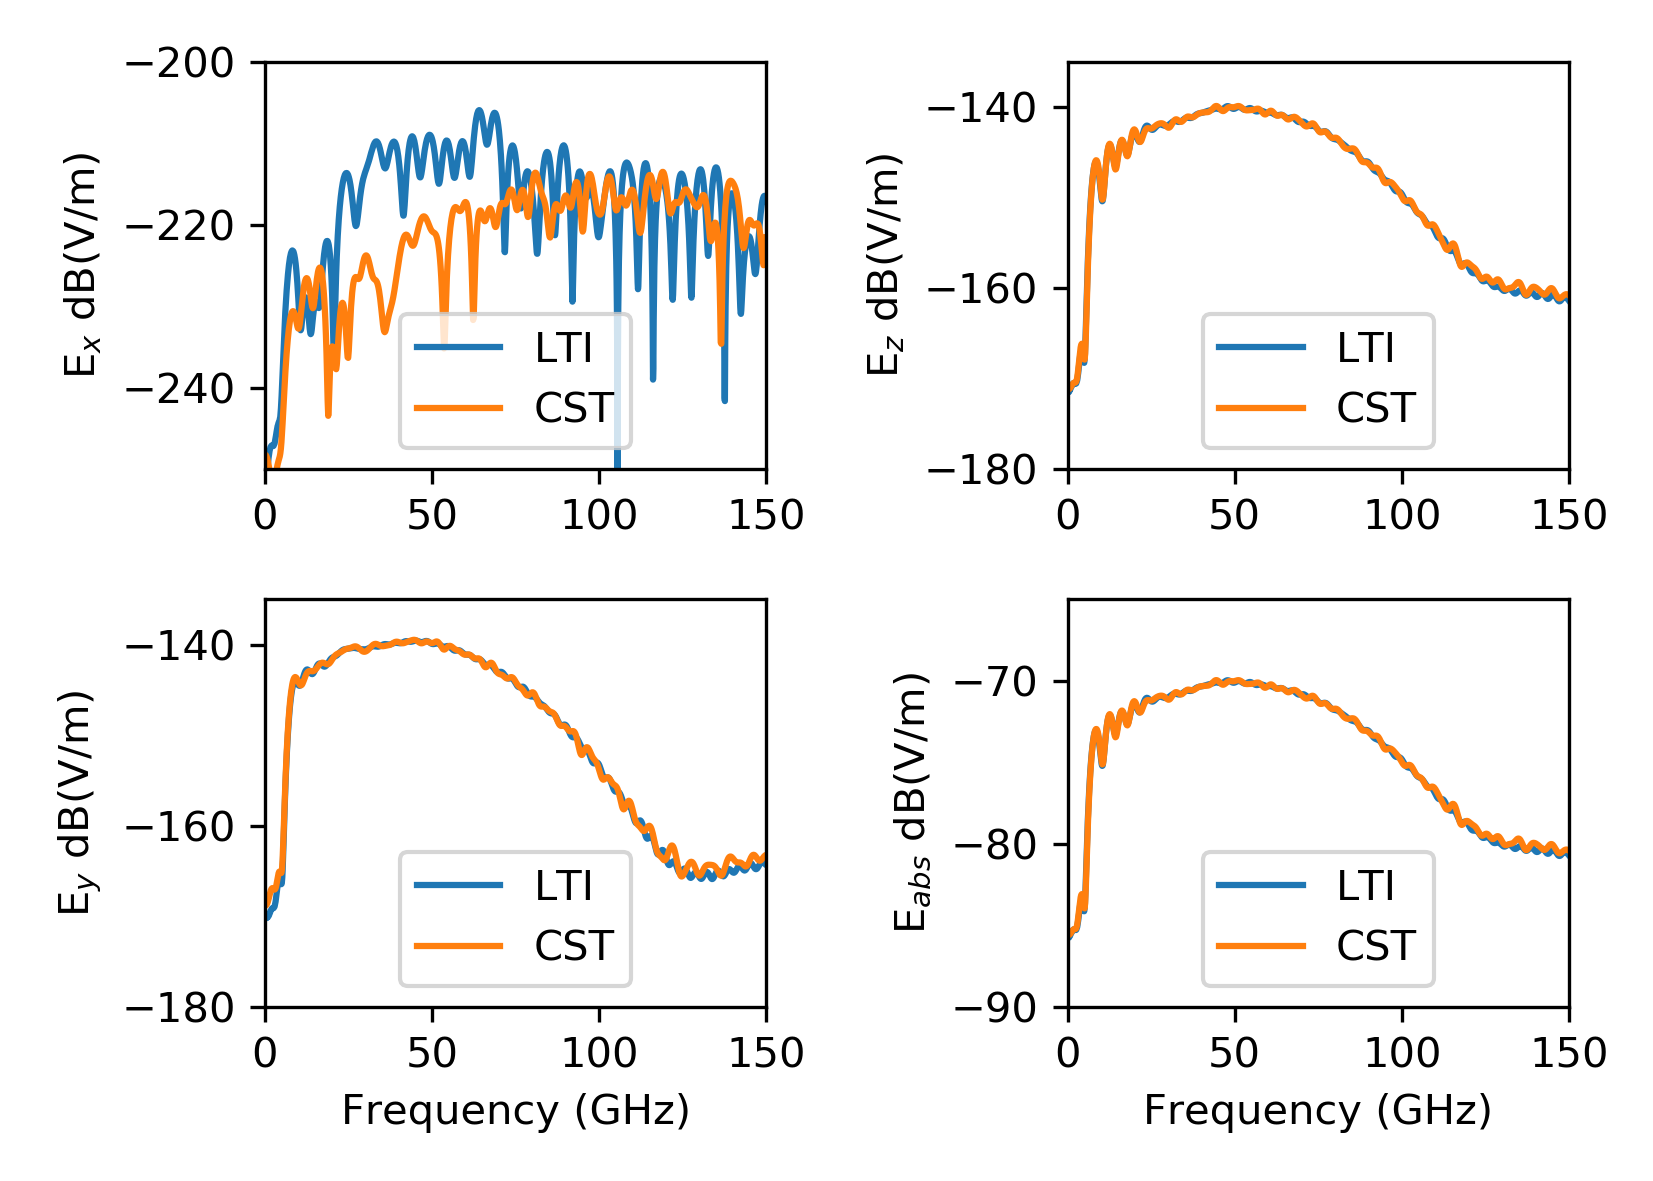
\includegraphics[scale=1, keepaspectratio]{pictures/LTI_reconstruction}
\caption{Electric field components in a point of the space calculated by means of a 3D simulation (CST) and using the convolution method (LTI). In both cases, the same 100~pC  2~ps Gaussian beam profile was used to run the full CST simulation and as input of the convolution method.
}\label{fig:LTI}
\end{figure}




\subsubsection{Transferring the results within the simulations}

As discussed previously, the simulation volume is critical in modelling the design of this device. However, the simulation can actually be split into two separate parts. The core of the simulation is the ChDR and DR production in the first part of the radiator. After that, the radiation fronts propagate in the radiator body similarly to inside a loaded waveguide. Therefore, the simulation process can be divided in two smaller simulations: 
\begin{enumerate}
\item Simulate with wakefield solver the beam interaction with the radiator surface, and sample the electric and magnetic fields after a short propagation space inside the radiator. The sampled fields are exported to text files.
\item Import the fields in a separate time-domain simulation that will simulate the propagation of the field through the radiator. 
\end{enumerate}
This approach is particularly advantageous. First, any simulation code can be used to simulate the beam-material interaction (step 1.). Secondly, if the shape of the radiator is modified, but the area exposed to the beam does not change, there is no need to run the first simulation again. 

This procedure was successfully implemented by means of export and import of the electric and magnetic fields to ASCII files. However, this experience showed that to avoid the creation of artifacts, a very fine and uniform spatial sampling of the fields recorded at the exit of the first step in the simulation 1 is essential.

Although these initial studies were successful in simple geometries with uniform meshing, it is not possible to extend this approach to models with a more complicated geometry (e.g. circular) while retaining the uniform meshing. To accomplish this with complicated geometries, it is necessary to get access to the mesh cells coordinates, which is not possible via the CST front-end. Further studies are planned in the future, in particular with the goal of using the IW2D~\cite{IW2D} code to simulate the beam-material interaction and then evaluate the propagation through the radiator. These studies showed that overcoming the limitations of commercial simulation codes is possible, however it requires to access the source code, that is not freely available to the user.









\section[Test in air]{Test in air}\label{sec:test-in-air}

\subsection[Experimental setup]{Experimental setup}\label{sec:setup}

The test device was installed in the CLEAR facility at CERN \cite{Sjobak:2019may}, in the so-called in-air test stand \cite{Corsini:IPAC2018-THPMF014}. A high-energy electron beam was produced in the CLEAR linac, and sent towards the end of the beamline where it exited into air through a thin metal window. The beam travels in air for approximately two metres before encountering the beam dump. This space was used to install the test device on translation stages remotely controllable with micron resolution. The transverse position of the device could be scanned around the beam in both the transverse directions independently over a span of 25~mm. By doing so, there was no need to modify the beam trajectory to carry out the tests. The achievable beam parameters that can be produced at CLEAR are reported in Table~\ref{tab:CLEAR_param}.

\begin{table}[b]
  \centering
    \begin{tabular}{l c c c}
    \toprule
    Parameter & Value \\
    \midrule
    Beam energy & 60 - 220 MeV\\
    Bunch charge & 10 pC - 2 nC\\
    Bunch length &1 – 4 ps\\
    Bunch frequency & 1.5 GHz\\
    RF frequency & 3.0 GHz\\
    Number of bunches & 1 - 200 \\
    Beam repetition rate & 0.83 – 10 Hz\\
    RMS energy spread & < 0.2 \% \\
    \bottomrule
    \end{tabular}
  \caption{Beam parameters achievable at the CLEAR facility \cite{Sjobak:2019may}.} \label{tab:CLEAR_param}
\end{table}

\begin{figure}[t]
\centering
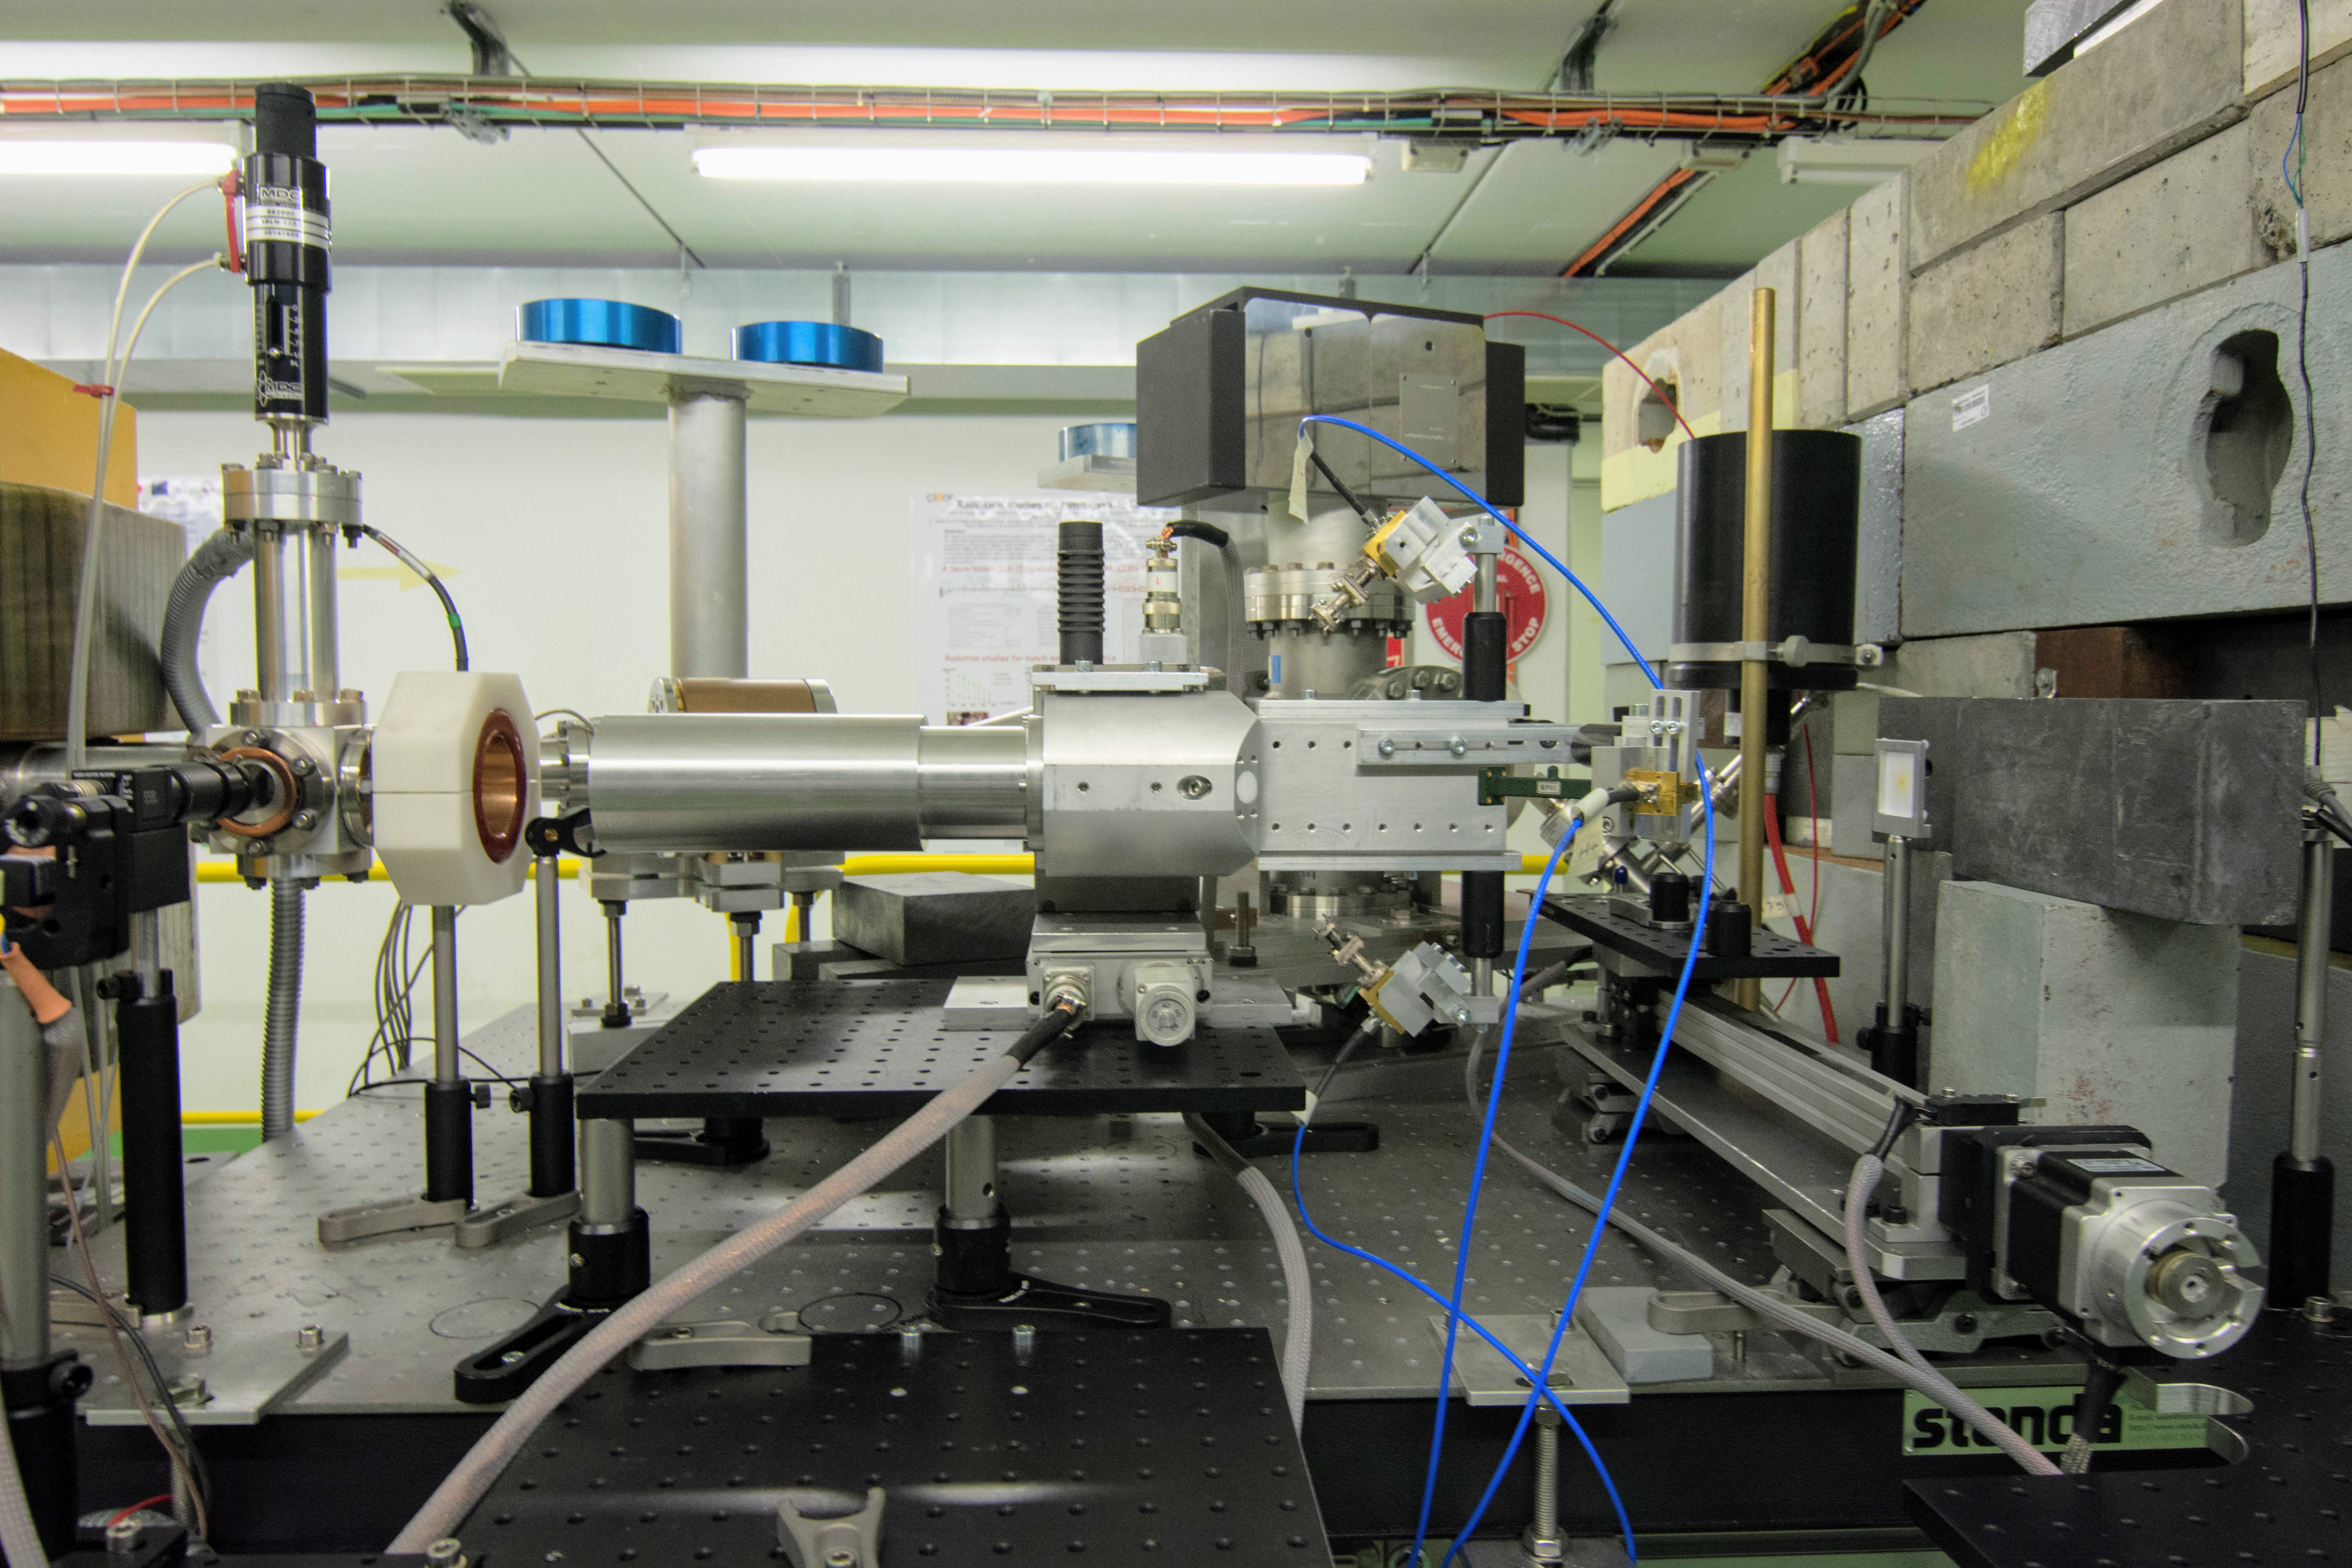
\includegraphics[width=13cm, keepaspectratio]{pictures/clear_installation}
\caption{The test device installed in the CLEAR in-air test stand. The beam exits the vacuum chamber on the left and passes through the white Integrating Current Transformer. It passes through the test device and reaches the lead and concrete beam dump on the right after hitting the small white screen. The blue cables connect the RF detectors to the signal acquisition chain. In the centre, the translation stage is visible.}
\label{fig:clear_installation}

% \vspace{5mm}

%     \begin{tabular}{l c c c}
%     \toprule
%     Plane & Diode model & Frequency band  \\
%     \midrule
%     Horiz. & Millitech DXP28-SPFW0 & Ka band (26.5-40 GHz)\\
%     \multirow{2}{*}{Vert.} & Millitech DXP15-SPFW0 & \multirow{2}{*}{V band (50-75 GHz)}\\
%      & Millitech DXP15-SNNW0 & \\


%     \bottomrule
%     \end{tabular}
%   \captionof{table}{RF diode detectors specifications.} \label{tab:diodes_planes}


\end{figure}




The installed test device can be seen in Fig.~\ref{fig:clear_installation}. The window through which the beam exits the vacuum chamber is on the left-hand side. The beam proceeds through the white ring, which is an Integrating Current Transformer~\cite{Clear:ICT} that measures the charge of each bunch train. Then the beam traverses the test device, hits the white beam screen on the right-hand side of the figure and is finally dumped on the lead and concrete absorber. The components installed in-air are aligned using an alignment laser.

The electromagnetic field produced by the test device was measured using zero-bias RF Schottky diode detectors. The advantages of such detectors include their relative simplicity and  being fitted with a waveguide input and a coaxial output. Detailed characterisation of these detectors will be presented in Section~\ref{sec:diodes}.

In order to maximise the frequency range accessible during the experiment, two pairs of RF diodes working in different frequency bands were chosen for the horizontal and vertical planes as reported in Table~\ref{tab:diodes_planes}. The detection was carried out in the Ka~band (26.5-40 GHz) in the horizontal plane, and in the V~band (50-75 GHz) in the vertical plane. In the horizontal plane, both the RF diodes were of the same model. On the other hand, in the vertical plane, one diode detected the full band (DXP15-SPFW0), while the other was narrow band (DXP15-SNNW0). The implications of this difference for the output signal will be discussed later.


\begin{table}[t]
\centering
    \begin{tabular}{l c c c}
    \toprule
    Plane & Diode model & Frequency band  \\
    \midrule
    Horiz. & Millitech DXP28-SPFW0 & Ka band (26.5-40 GHz)\\
    \multirow{2}{*}{Vert.} & Millitech DXP15-SPFW0 & \multirow{2}{*}{V band (50-75 GHz)}\\
     & Millitech DXP15-SNNW0 & \\


    \bottomrule
    \end{tabular}
  \captionof{table}{RF diode detectors specifications.} \label{tab:diodes_planes}
\end{table}


Some preliminary tests immediately showed that the RF diodes easily saturate with the high peak power produced by the ChDR radiators of the test device, making them unusable for precise measurements. Therefore, to prevent saturation, the horn antennas initially installed in front of the diodes were removed, and a waveguide attenuator was added in front of the Ka-band diodes installed on the horizontal plane of the test device. The attenuation was adapted according to the beam charge in the range from 10 to 30 dB. Suitable waveguide attenuators were not available for the RF diodes installed in the vertical plane and  a standard waveguide was used instead. The waveguide equipment installed in front of the RF diodes acted as highpass filters. In the horizontal plane only frequencies above the 21~GHz cut-off frequency of a WR28 waveguide could reach the diodes. Similarly, in the vertical plane, only frequencies above the 39.9 GHz cut-off frequency of a WR15 waveguide reached the diodes.


The signal detection and acquisition chain is presented in Fig.~\ref{fig:scheme_acquisition} for the Ka- and V-band implementations. The signal from each Ka-band RF detector was sent via a short cable to an amplifier placed under the test stand to shield it from background radiation. The amplified signal was then sent via a long coaxial cable to a fast oscilloscope located outside the accelerator tunnel. No amplifier was used for the V-band detectors and their signal was acquired directly by the same oscilloscope. 

\begin{figure}[t]
\centering
\begin{tikzpicture}[line cap=round,line join=round,>=triangle 45,x=1cm,y=1cm, scale=0.5, every node/.style={scale=.8}]

\clip(-8,-4.) rectangle (18,4);

\draw [shift={(-10,0)},line width=1pt]  plot[domain=-0.46364760900080615:0.4636476090008061,variable=\t]({1*4.47213595499958*cos(\t r)+0*4.47213595499958*sin(\t r)},{0*4.47213595499958*cos(\t r)+1*4.47213595499958*sin(\t r)});
\draw [shift={(-8,0)},line width=1pt]  plot[domain=-0.46364760900080615:0.4636476090008061,variable=\t]({1*4.47213595499958*cos(\t r)+0*4.47213595499958*sin(\t r)},{0*4.47213595499958*cos(\t r)+1*4.47213595499958*sin(\t r)});
\draw [shift={(-9,0)},line width=1pt]  plot[domain=-0.46364760900080615:0.4636476090008061,variable=\t]({1*4.47213595499958*cos(\t r)+0*4.47213595499958*sin(\t r)},{0*4.47213595499958*cos(\t r)+1*4.47213595499958*sin(\t r)});

\draw [line width=1pt] (-1,1)-- (0,0);
\draw [line width=1pt] (-1,-1)-- (0,0);
\draw [line width=1pt] (0,0)-- (2,0);
\draw [line width=1pt] (2,0)-- (2,0.5);
\draw [line width=1pt] (2,0)-- (2,-0.5);
\draw [line width=1pt] (2,-0.5)-- (5,-0.5);
\draw [line width=1pt] (5,-0.5)-- (5,0.5);
\draw [line width=1pt] (5,0.5)-- (2,0.5);
\draw [line width=1pt] (5,0)-- (7,0);
\draw [line width=1pt] (7,0)-- (7,1);
\draw [line width=1pt] (7,1)-- (9,1);
\draw [line width=1pt] (9,1)-- (9,0);
\draw [line width=1pt] (9,0)-- (9,-1);
\draw [line width=1pt] (9,-1)-- (7,-1);
\draw [line width=1pt] (7,-1)-- (7,0);
\draw [line width=1pt] (9,0)-- (11,0);

\draw [line width=1pt] (11,0)-- (11,1);
\draw [line width=1pt] (11,1)-- (12,0);
\draw [line width=1pt] (12,0)-- (11,-1);
\draw [line width=1pt] (11,-1)-- (11,0);

\draw [line width=1pt] (12,0)-- (14,0);
\draw [line width=1pt] (14,0)-- (14,1);
\draw [line width=1pt] (14,1)-- (16,1);
\draw [line width=1pt] (16,1)-- (16,-1);
\draw [line width=1pt] (16,-1)-- (14,-1);
\draw [line width=1pt] (14,0)-- (14,-1);
\draw [line width=1pt] (7.2,0.4)-- (7.6,0.4);
\fill[line width=1pt, fill=black, fill opacity=1] (7.6,0.2) -- (7.6,0.6) -- (7.8,0.4) -- cycle;
\draw [line width=1pt] (7.8,0.4)-- (7.8,0.6);
\draw [line width=1pt] (7.8,0.4)-- (7.8,0.2);
\draw [line width=1pt] (7.8,0.4)-- (8.8,0.4);
\draw [line width=1pt] (8.2,0.4)-- (8.2,0);
\draw [line width=1pt] (8.2,0)-- (8,0);
\draw [line width=1pt] (8.2,0)-- (8.4,0);
\draw [line width=1pt] (8,-0.2)-- (8.2,-0.2);
\draw [line width=1pt] (8.2,-0.2)-- (8.4,-0.2);
\draw [line width=1pt] (8.2,-0.2)-- (8.2,-0.6);

% \draw [->,line width=0.6pt] (14.2, 0) -- (15.8, 0);
% \draw [->,line width=0.6pt] (15, -0.8) -- (15, 0.8);


\draw (-5.7,4.) node[anchor=north west] {RF};
\draw (-5.,-2) node[anchor=north west] {\parbox{5 cm}{\centering Horn Antenna \\(Optional)}};
\draw (-1,4) node[anchor=north west] {\parbox{5 cm}{\centering Waveguide \\ Attenuator \\ 10-30 dB}};
\draw (6.5,-2) node[anchor=north west] {\parbox{4 cm}{ Ka Band\\Detector}};
\draw (8.,4) node[anchor=north west] {\parbox{4cm}{\centering Amplifier\\14 dB}};
\draw (11.8,-2) node[anchor=north west] {\parbox{4cm}{\centering Oscilloscope}};

\draw [dashed, line width=1pt] (13,1.25)-- (13,-4);

\draw [line width=1pt] (14.2,-.8)-- (14.2,0.8);
\draw [line width=1pt] (14.2,0.8) -- (15.8,0.8);
\draw [line width=1pt] (15.8,0.8)-- (15.8,-0.8);
\draw [line width=1pt] (14.2,-0.8)-- (15.8,-0.8);

\draw [line width=1pt] (14.4,0)-- (14.6,0);
\draw [line width=1pt] (14.6,0)-- (14.65,-0.2);
\draw [line width=1pt] (14.65,-0.2)-- (14.8,0);
\draw [line width=1pt] (14.8,0)-- (15.05,0);
\draw [line width=1pt] (15.05,0)-- (15.2,0.4);
\draw [line width=1pt] (15.2,0.4)-- (15.5,0);
\draw [line width=1pt] (15.5,0)-- (15.6,0);

\end{tikzpicture}

\begin{tikzpicture}[line cap=round,line join=round,>=triangle 45,x=1cm,y=1cm, scale=0.5, every node/.style={scale=.8}]

\clip(-8,-4.) rectangle (18,4);

\draw [shift={(-10,0)},line width=1pt]  plot[domain=-0.46364760900080615:0.4636476090008061,variable=\t]({1*4.47213595499958*cos(\t r)+0*4.47213595499958*sin(\t r)},{0*4.47213595499958*cos(\t r)+1*4.47213595499958*sin(\t r)});
\draw [shift={(-8,0)},line width=1pt]  plot[domain=-0.46364760900080615:0.4636476090008061,variable=\t]({1*4.47213595499958*cos(\t r)+0*4.47213595499958*sin(\t r)},{0*4.47213595499958*cos(\t r)+1*4.47213595499958*sin(\t r)});
\draw [shift={(-9,0)},line width=1pt]  plot[domain=-0.46364760900080615:0.4636476090008061,variable=\t]({1*4.47213595499958*cos(\t r)+0*4.47213595499958*sin(\t r)},{0*4.47213595499958*cos(\t r)+1*4.47213595499958*sin(\t r)});

\draw [line width=1pt] (-1,1)-- (0,0);
\draw [line width=1pt] (-1,-1)-- (0,0);
\draw [line width=1pt] (0,0)-- (2,0);
\draw [line width=1pt] (2,0)-- (2,0.5);
\draw [line width=1pt] (2,0)-- (2,-0.5);
\draw [line width=1pt] (2,-0.5)-- (5,-0.5);
\draw [line width=1pt] (5,-0.5)-- (5,0.5);
\draw [line width=1pt] (5,0.5)-- (2,0.5);
\draw [line width=1pt] (5,0)-- (7,0);
\draw [line width=1pt] (7,0)-- (7,1);
\draw [line width=1pt] (7,1)-- (9,1);
\draw [line width=1pt] (9,1)-- (9,0);
\draw [line width=1pt] (9,0)-- (9,-1);
\draw [line width=1pt] (9,-1)-- (7,-1);
\draw [line width=1pt] (7,-1)-- (7,0);
\draw [line width=1pt] (9,0)-- (11.5,0);
% \draw [line width=1pt] (11,0)-- (11,0.5);
% \draw [line width=1pt] (11,0.5)-- (11.5,0);
% \draw [line width=1pt] (11.5,0)-- (11,-0.5);
% \draw [line width=1pt] (11,-0.5)-- (11,0);
\draw [line width=1pt] (11.5,0)-- (14,0);
\draw [line width=1pt] (14,0)-- (14,1);
\draw [line width=1pt] (14,1)-- (16,1);
\draw [line width=1pt] (16,1)-- (16,-1);
\draw [line width=1pt] (16,-1)-- (14,-1);
\draw [line width=1pt] (14,0)-- (14,-1);
\draw [line width=1pt] (7.2,0.4)-- (7.6,0.4);
\fill[line width=1pt, fill=black, fill opacity=1] (7.6,0.2) -- (7.6,0.6) -- (7.8,0.4) -- cycle;
\draw [line width=1pt] (7.8,0.4)-- (7.8,0.6);
\draw [line width=1pt] (7.8,0.4)-- (7.8,0.2);
\draw [line width=1pt] (7.8,0.4)-- (8.8,0.4);
\draw [line width=1pt] (8.2,0.4)-- (8.2,0);
\draw [line width=1pt] (8.2,0)-- (8,0);
\draw [line width=1pt] (8.2,0)-- (8.4,0);
\draw [line width=1pt] (8,-0.2)-- (8.2,-0.2);
\draw [line width=1pt] (8.2,-0.2)-- (8.4,-0.2);
\draw [line width=1pt] (8.2,-0.2)-- (8.2,-0.6);

\draw [line width=1pt] (14.2,-.8)-- (14.2,0.8);
\draw [line width=1pt] (14.2,0.8) -- (15.8,0.8);
\draw [line width=1pt] (15.8,0.8)-- (15.8,-0.8);
\draw [line width=1pt] (14.2,-0.8)-- (15.8,-0.8);

\draw [line width=1pt] (14.4,0)-- (14.6,0);
\draw [line width=1pt] (14.6,0)-- (14.65,-0.2);
\draw [line width=1pt] (14.65,-0.2)-- (14.8,0);
\draw [line width=1pt] (14.8,0)-- (15.05,0);
\draw [line width=1pt] (15.05,0)-- (15.2,0.4);
\draw [line width=1pt] (15.2,0.4)-- (15.5,0);
\draw [line width=1pt] (15.5,0)-- (15.6,0);


\draw (-5.7,4.) node[anchor=north west] {RF};
\draw (-5.,-2) node[anchor=north west] {\parbox{5 cm}{\centering Horn Antenna \\(Optional)}};
\draw (-1,3) node[anchor=north west] {\parbox{5 cm}{\centering WR15 \\ Waveguide}};
\draw (6.5,-2) node[anchor=north west] {\parbox{4 cm}{ V Band\\Detector}};
\draw (11.8,-2) node[anchor=north west] {\parbox{4cm}{\centering Oscilloscope}};


\draw [dashed, line width=1pt] (13.13,-1.25)-- (13.13,3);
\draw (11.3, 4.2) node[anchor=north west] {\parbox{4cm}{\centering \textbf{Service\\Gallery}}};
\draw (8, 4) node[anchor=north west] {\parbox{4cm}{\centering \textbf{Bunker}}};

\end{tikzpicture}
\caption{Schematic representation of the ChDR signal detection used for the experiments. The Ka-band acquisition system used for the horizontal plane is represented on the top. The V-band acquisition for the vertical plane is drawn on the bottom.}
\label{fig:scheme_acquisition}
\end{figure}

The dual-channel amplifier used was custom made for an earlier project. Before using it for the ChDR application, the amplifier was characterised in-situ using a portable 20~GHz bandwidth Vector Network Analyser. The measurements showed a bandwidth of 1.3~GHz and a gain of 13.9~dB on one channel and 1.2~GHz bandwidth and 14.3~dB gain on the other channel. A high-resolution, fast-sampling and remotely controllable oscilloscope was used to acquire the data. Depending on the test, it was set to 12~bit resolution and 4~GHz analog bandwidth, or 8~bit resolution and 6~GHz analog bandwidth.

\subsection[RF Schottky-diode detectors]{RF Schottky-diode detectors}\label{sec:diodes}

The electromagnetic radiation produced by the test device was measured using commercial zero-bias RF detectors based on Schottky diodes that rectify the incoming RF wave, providing a signal proportional to the incident power. Such detectors are often employed to measure the power of Continuous Wave (CW) RF signals but can also be used to measure short pulses provided that the pulse length is considerably shorter than the detector rise time. RF diodes already available at CERN from other projects were used for characterising the test device at CLEAR. The sensors operating in the Ka~band were tested with a 40~GHz synthesizer but it was not possible to measure the detectors working in the V~band as no suitable test instrument was available.

To test the Ka-band RF diodes, an HP83642 40~GHz synthesizer was used. An HP~R281A adapter connected the 2.4~mm coaxial output of the synthesizer to the detector waveguide input. The synthesizer produced 5~$\mu$s-long RF pulses every 19~$\mu$s with the desired frequency and power. The diode output voltage was acquired with the oscilloscope described in Section~\ref{sec:setup}. Figure~\ref{fig:diode_cal_setup} shows the test setup and a typical diode output voltage. The signal was averaged over 50 acquisitions directly on the oscilloscope before saving the trace. The number of averaged acquisitions was determined empirically to achieve the maximum measurement noise reduction while being able to carry out the characterisation of both diodes in a single day. 

\begin{figure}[!t]
\centering
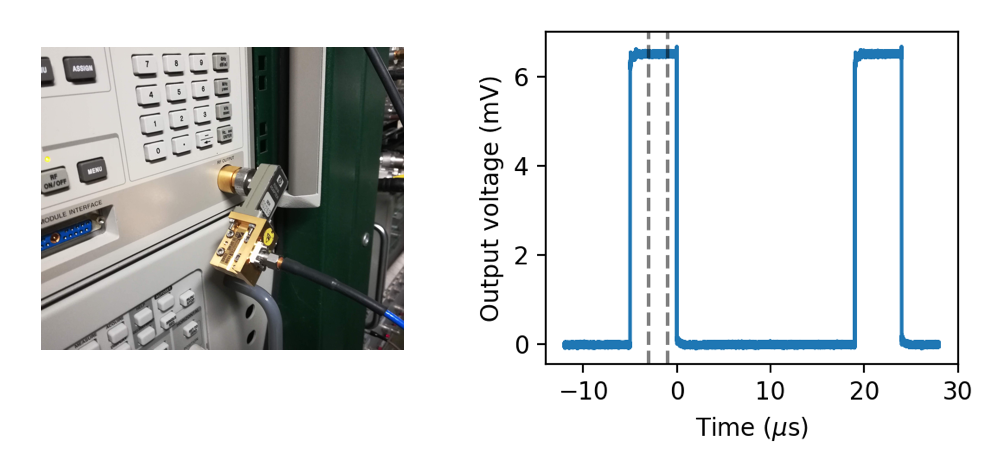
\includegraphics[scale=1,keepaspectratio]{pictures/diode_cal_single}
\caption{An RF diode installed on the synthesizer for calibration (left) and a typical diode output signal during calibration (right). Only the region between the dashed lines is taken into account to evaluate the average voltage output. The rise and fall of the pulse are discarded, as it is not possible to assess to which extent these are determined by the diode or the synthesizer. Additional details on the response of Schottky diodes to fast transients are given in Section~\ref{sec:diodes_leakage}.}
\label{fig:diode_cal_setup}
\end{figure}

The synthesizer and the oscilloscope were remotely controlled via GPIB~\cite{GPIB} and LXI~\cite{LXI} commands respectively from a remote computer using a custom script which set the power and frequency, sweeping the frequency between 26~and 40~GHz in steps of 1~GHz and the power between -14 and 3~dBm\footnote{The dBm is a common RF power unit expressed in decibels and normalised to 1 mW. For reference, 0 dBm = 1 mW, and -10 dBm = 0.1 mW.} in steps of 1~dBm. The diode output voltage was calculated as the average voltage in a 2~$\mu$s window after the initial transients. The considered window is marked by the two vertical bars in Fig.~\ref{fig:diode_cal_setup}. 




The response of an ideal RF diode detector based on a Schottky diode is well known from simple equivalent circuit models \cite{schottky_diodes_temp_extremes}. At low power levels, the response is linear with the input power. This regime is called the `square law region' as the voltage output is proportional to the square of the input voltage. For the detectors used at CLEAR, the linear region extends up to input power of -10~dBm \cite{diodes_datasheet} (0.1~mW). With higher input power, the response becomes non linear. After an initial transition, the device enters a nonlinear region where the output voltage is proportional to the square root of the input power. These two regions are called the `transition region' and the `linear region' (as the output voltage is linear with the input voltage). At very high input power the diodes saturate and eventually they might be permanently damaged. 

The calibration results are shown in Fig.~\ref{fig:diode_cal_data}. The tested RF diodes' response is linear up to input power of 0.1~mW, or -10~dBm, indicated by the dashed line agreeing with what is advertised by the manufacturer. Increasing the input power, the response becomes nonlinear and more frequency dependent. This is particularly visible in the right plot of Fig.~\ref{fig:diode_cal_data} at the operating band edge frequencies of 26 and 40 GHz, where the response kinks when surpassing 0.1~mW input power. A smoother response at the center of the frequency operating band is found, that likely depends on optimisations performed in the device design. 


\begin{figure}[!b]
\centering
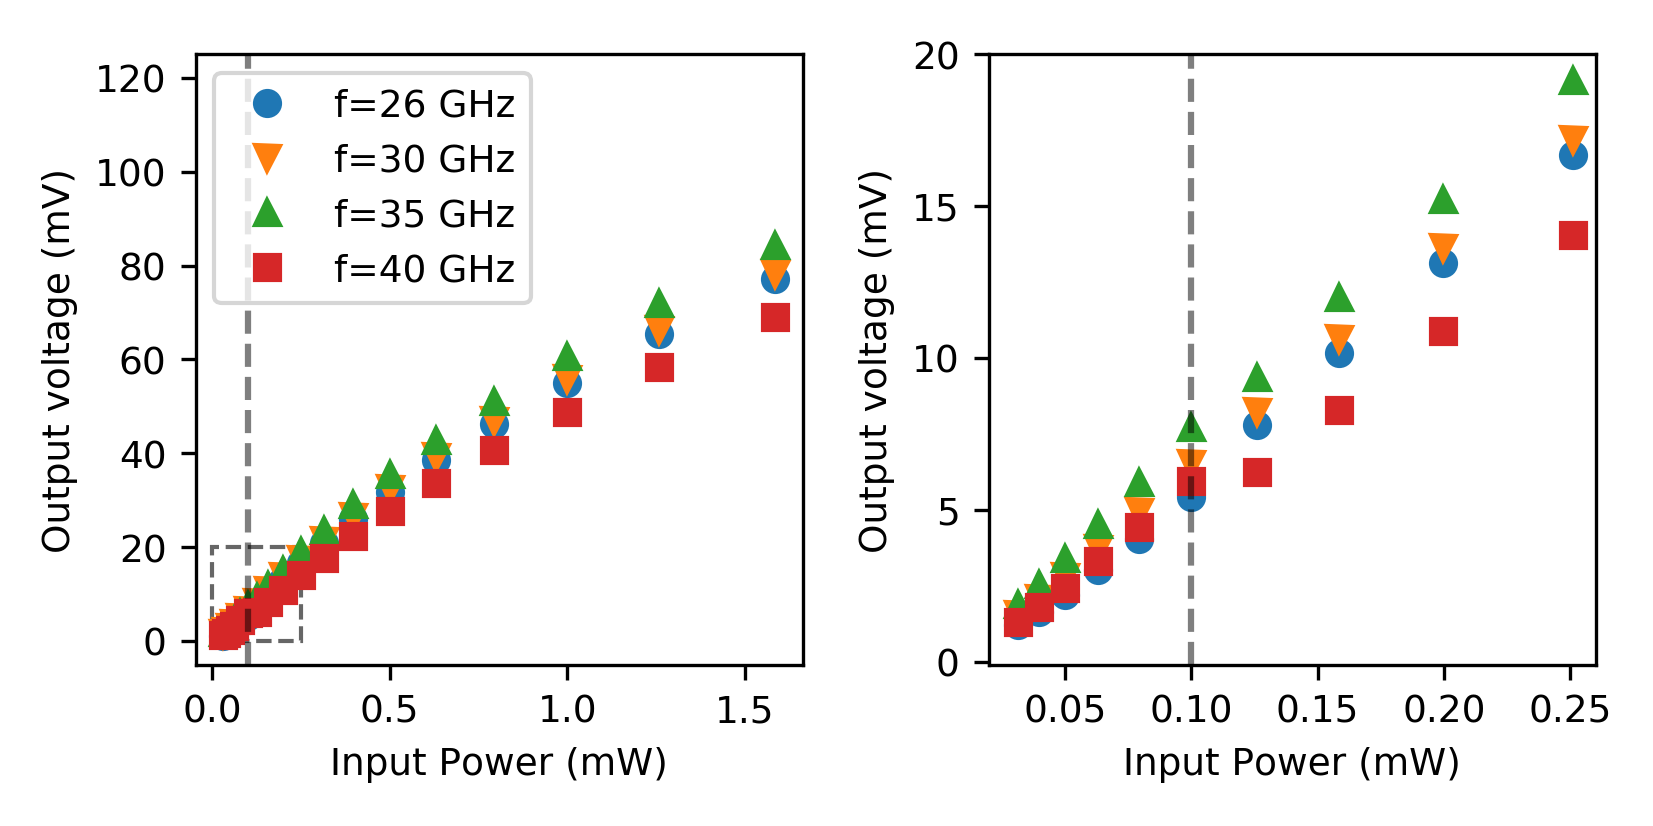
\includegraphics[scale=1, keepaspectratio]{pictures/diode_cal_data}
\caption{Diode response to the CW RF input produced by the synthesizer. The vertical dashed line indicates the linearity limit of 0.1~W indicated by the manufacturer. The response at different input frequencies is shown. The left plot shows the full tested range. The dashed box shows the reduced data range shown in the right plot.}\label{fig:diode_cal_data}
\end{figure}


The RF diode averaged response was calculated to identify the linear and non-linear working regions and the transition region between them. For each input power level, the mean and standard error of the mean of the acquired responses were computed and are shown in Figure~\ref{fig:diode_cal_fits}. A linear and square root function were fitted to the data in the respective working regions. The linear region is on the left-hand side of the plot. The transition region can be seen between approximately 0.1-0.3~mW (-10 and -6~dBm) input power. The linear fit was calculated for input power $<0.1$~mW. Statistical analysis showed that by extending this linear behaviour to higher input power, the residual error on the fit is below $5\%$ up to 0.4~mW.



\begin{figure}[!t]
\centering
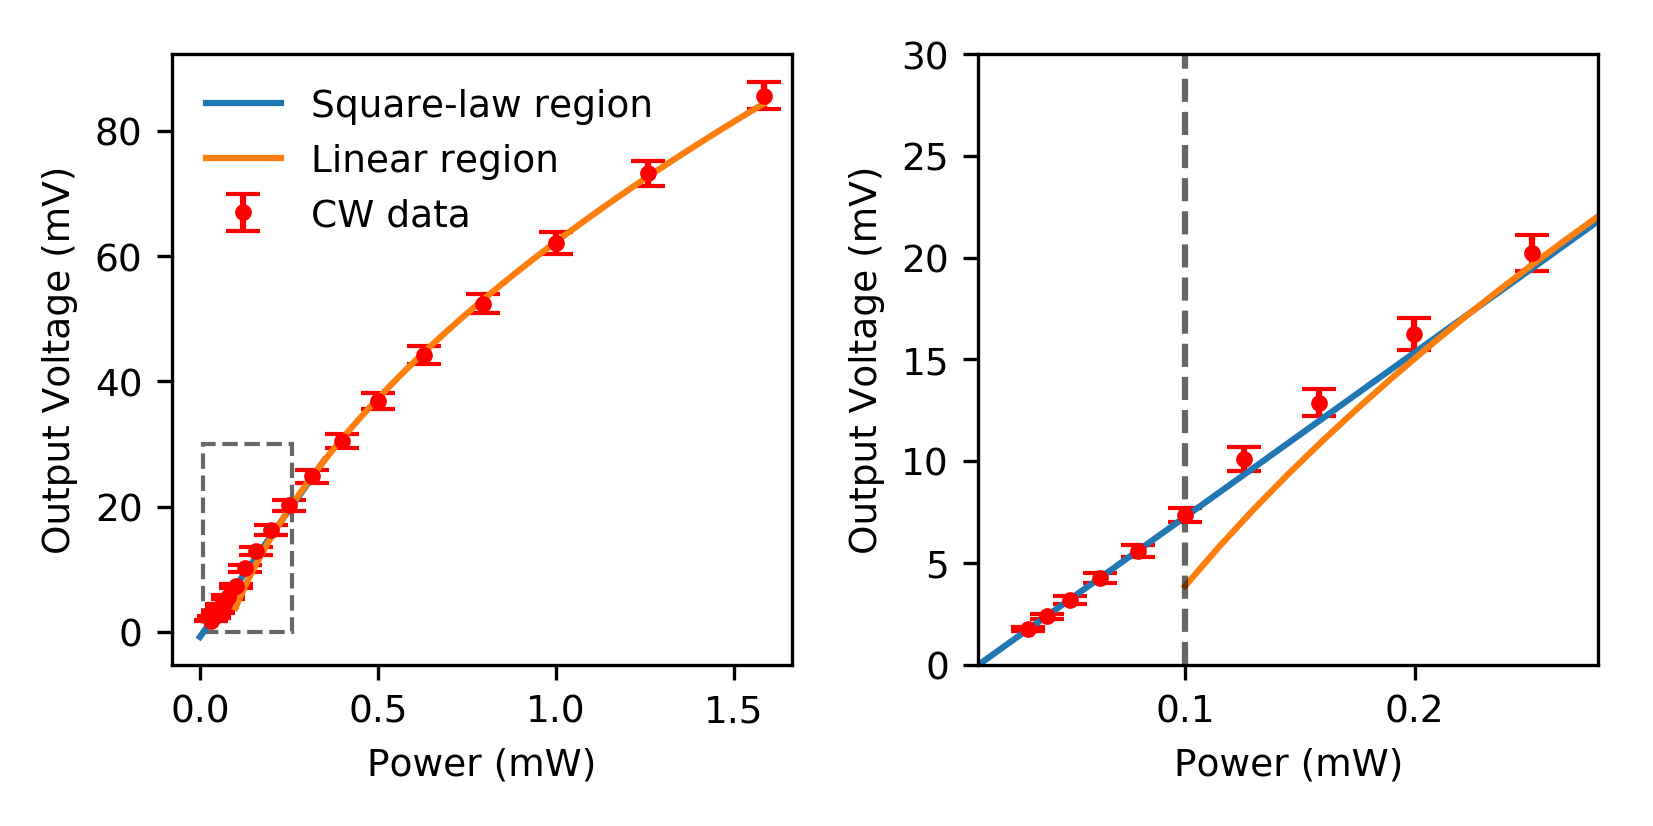
\includegraphics[scale=1, keepaspectratio]{pictures/diode_cal_fit3}
\caption{Tested Schottky-diode average response to CW RF input from the synthesizer. The vertical dashed line delimits the linear region. The left plot shows the full tested range, while the right plot zooms on the low input power range indicated by the dashed box. The bars represent the standard error of the mean output voltage at each input power.}
\label{fig:diode_cal_fits}
\end{figure}

After preliminary tests, the signals sent to the diodes were attenuated to avoid saturation. For the results presented in this work, the diode output voltage never exceeded 15~mV, so it can be assumed that the diodes worked in their linear region. Unfortunately, no reference in literature was found for characterisation of Schottky diode detectors with short RF pulses. However, in this work the diode detector response is assumed to be linear for the power levels produced by the ChDR.






\subsection{Beam position response for single bunch beam}\label{sec:single_bunch}

The primary goal of the tests was to assess whether ChDR emission can be used to measure the transverse position of an electron beam. For this purpose, an electron beam with energy exceeding 200~MeV, a bunch charge between 10 and 200~pC and a bunch length of 2~ps was used. Slight variations of these parameters were anticipated due to the varying bunch charge which was recorded shot-by-shot. The beam was kept at a constant transverse position, and the test device was moved around it by motorized translation stages. 


A beam consisting of a single bunch was used to test the device response with two values of the beam charge and over two different position ranges. Table~\ref{tab:1bunch_test_param} shows the parameters of the four tests. A comparison of the spanned position range in the different tests is presented in Fig.~\ref{fig:datasets_comparison_1b}.

\begin{table}[!ht]
  \centering
%   \vspace*{-6mm}
    \begin{tabular}{l c c c}
    \toprule
    Dataset name & Charge (pC) & Position scan range  \\
    \midrule
    coarse scan  & $35\pm7$ & 25 mm\\
    fine scan    & $37\pm7$ & 4.5 mm\\
    finest scan  & $41\pm7$ & 2.5 mm\\
    fine scan low charge  & $12.6\pm1.9$ & 4.5 mm\\
    100$\mu$m low charge  & $10-15$ (est.) & 1.5 mm\\
    \bottomrule
    \end{tabular}
  \caption{Parameters of the tests with a single bunch beam. The charge for the dataset `100$\mu$m low charge' was not recorded, but the settings of the preceding dataset were retained. It can therefore be assumed that the charge was between 10 and 15~pC per bunch.} \label{tab:1bunch_test_param}
  
%   \begin{figure}[!t]
% \centering
\vspace{-1mm}
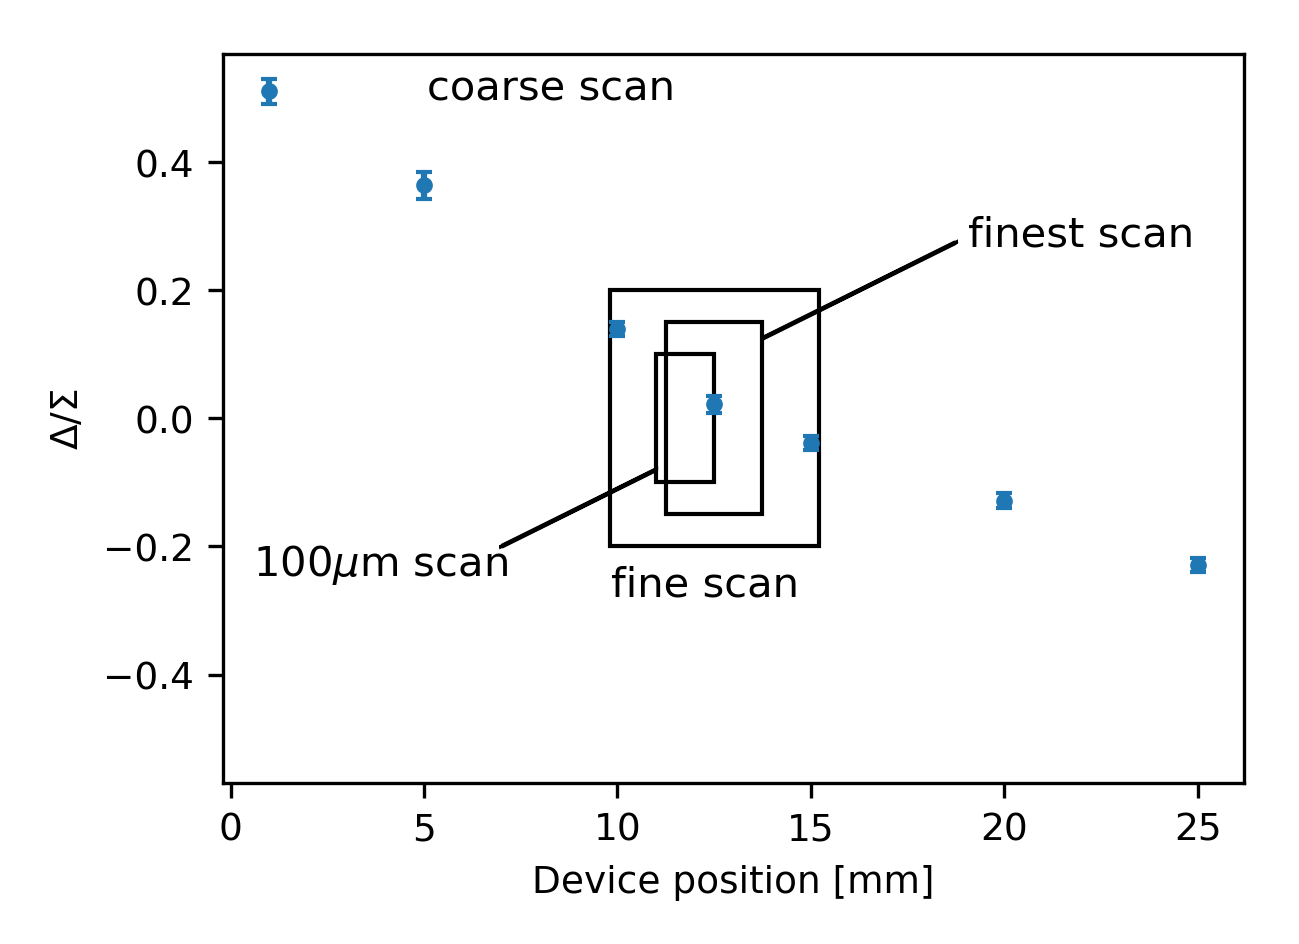
\includegraphics[scale=0.9, keepaspectratio]{pictures/coarse_vs_the_others}
\vspace*{-2mm}
\captionof{figure}{Comparison of the translation stage position range for different datasets. The `coarse scan' dataset spans over the whole translation stage range of 25~mm. The displayed data were processed with method~2 (presented later).}\label{fig:datasets_comparison_1b}
% \end{figure}


\end{table}

Data acquisition was controlled remotely via custom python scripts interfacing the CERN accelerator control system via pyJAPC \cite{pyJAPC}, setting the accelerator parameters, controlling the translation stages, and managing the oscilloscope. 


The large amount of data produced was saved locally on the oscilloscope and later copied to the CERN infrastructure for processing using the following procedure:
\begin{enumerate}
    \item The oscilloscope saves the recoded data at each beam passage to four comma-separated value files, one per channel. The files are timestamped using the oscilloscope's local time accurate to the second. At the same time, the beam charge and readings of other diagnostic devices, such as the beam screen images, are stored in the CERN infrastructure by the CLEAR acquisition system.
    \item All the data are copied to a common location. The oscilloscope files are opened one by one, and one Pandas \cite{pandas} DataFrame per scope channel is assembled. Each of them contains the oscilloscope trace matched to its timestamp and the translation stages position. The timestamp is used to match the beam charge measured at that time. 
    \item The data are then saved to a new single DataFrame creating a single event structure. At each `event', i.e. each beam passage, a common timestamp is used for the four oscilloscope traces, beam charge and translation-stage position.
    \item For the signals of the Ka-band detectors the amplifier gain and baseline are removed. 
\end{enumerate}
Throughout this process, the data quality was assessed and the events where the oscilloscope was saturated or the acquisition was faulty were eliminated. Typically, for each translation stage position, 50 events were acquired. If some event was deleted during the processing, the reduction of the number of samples was taken into account in the analysis. An example of the signal produced by the ChDR emission picked up by a diode detector is presented in Fig.~\ref{fig:diode_signal_1b}. 


\begin{figure}[!b]
\centering
\vspace{-1mm}
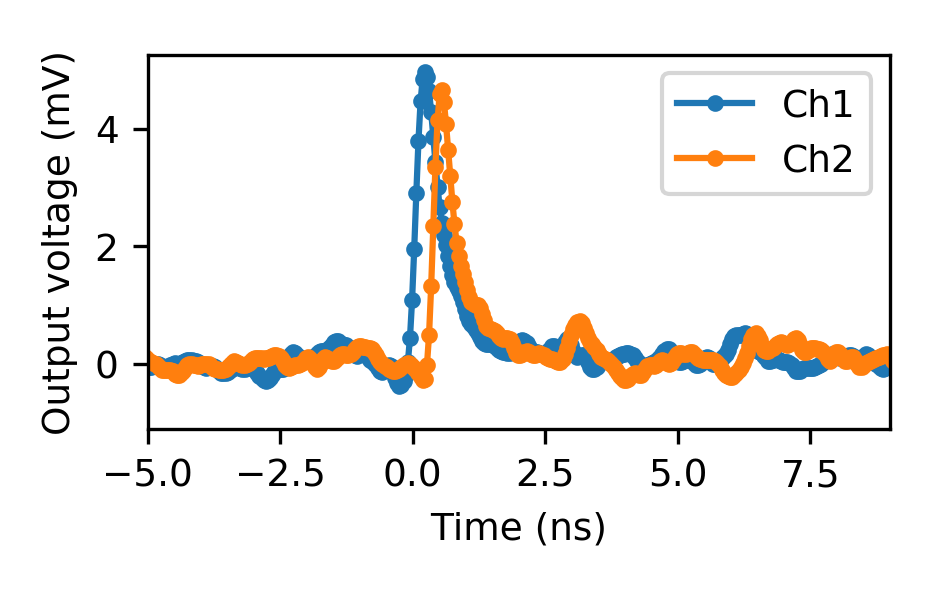
\includegraphics[scale=1, keepaspectratio]{pictures/single_bunch_scope}
\vspace*{-2mm}
\captionof{figure}{The output signal of the Ka~band diode detectors installed for the horizontal plane. The amplifier gain and baseline were removed. Some minor reflections due to the cable connections are visible, e.g. on channel 2 after 2.5~ns. The solid dots mark the oscilloscope sampling points.}
\label{fig:diode_signal_1b}
\end{figure}




A number of processing algorithms were tested and the ones found to be the most satisfactory are: 
\begin{description}
\item[Method 1: upsample, align and average.] Each trace is upsampled five times and the signal peaks are aligned for all events recorded at the same translation-stage position. The events are then averaged and a smaller time window of the signal is selected. The standard deviation of the windowed signal is calculated for both channels in the same plane. The quantity $\Delta/\Sigma$ is then calculated using the standard-deviation values. This method produces a single measurement per translation position stage. Therefore, a statistical error on the $\Delta/\Sigma$ cannot be calculated in this case. 
%
\item[Method 2: upsample and align.] The Method~1 procedure is followed but the signals are not averaged. Therefore, one value of $\Delta/\Sigma$ is produced per event.
%
\item[Method 3: data windowing only.] Each oscilloscope trace is windowed. The data are used to calculate the standard deviation and the $\Delta/\Sigma$ of each event.
\end{description}


All applied processing methods assume that the beam does not move during the measurement. Although the beam position monitoring was not available during these tests, it is likely that only limited drifts occurred as the measurements were taken during the night and the acquisition of each dataset takes $\sim10$ minutes, limiting the possible effect of thermal drifts of the accelerator. Furthermore, it is assumed that the detector response is linear and that the bunch-charge variation affects both detectors in the same way. 

The device was installed and aligned to the reference laser of the test stand with the best accuracy possible. The translation stage was set such that the 12.5~mm position corresponds to the laser in the center of the beampipe. Assuming that the reference laser and the beam are aligned, the 12.5~mm position corresponds to the quantity $\Delta/\Sigma=0$.

The results of the three processing methods for the `fine scan' dataset are shown in Fig.~\ref{fig:four_proc_1b} together with a linear fit. The fit parameters are reported in the first row of Table~\ref{tab:fit_four_proc_1b}. The derived beam position sensitivity is consistent for all processing methods. The average $\Delta/\Sigma$ sensitivity to the beam position is $(3.8\pm0.5)\times10^{-2}$ mm$^{-1}$ where the uncertainty is conservatively estimated using the Root Sum Square (RSS) of the uncertainties calculated individually for the three methods.

\begin{figure}[!t]
\centering
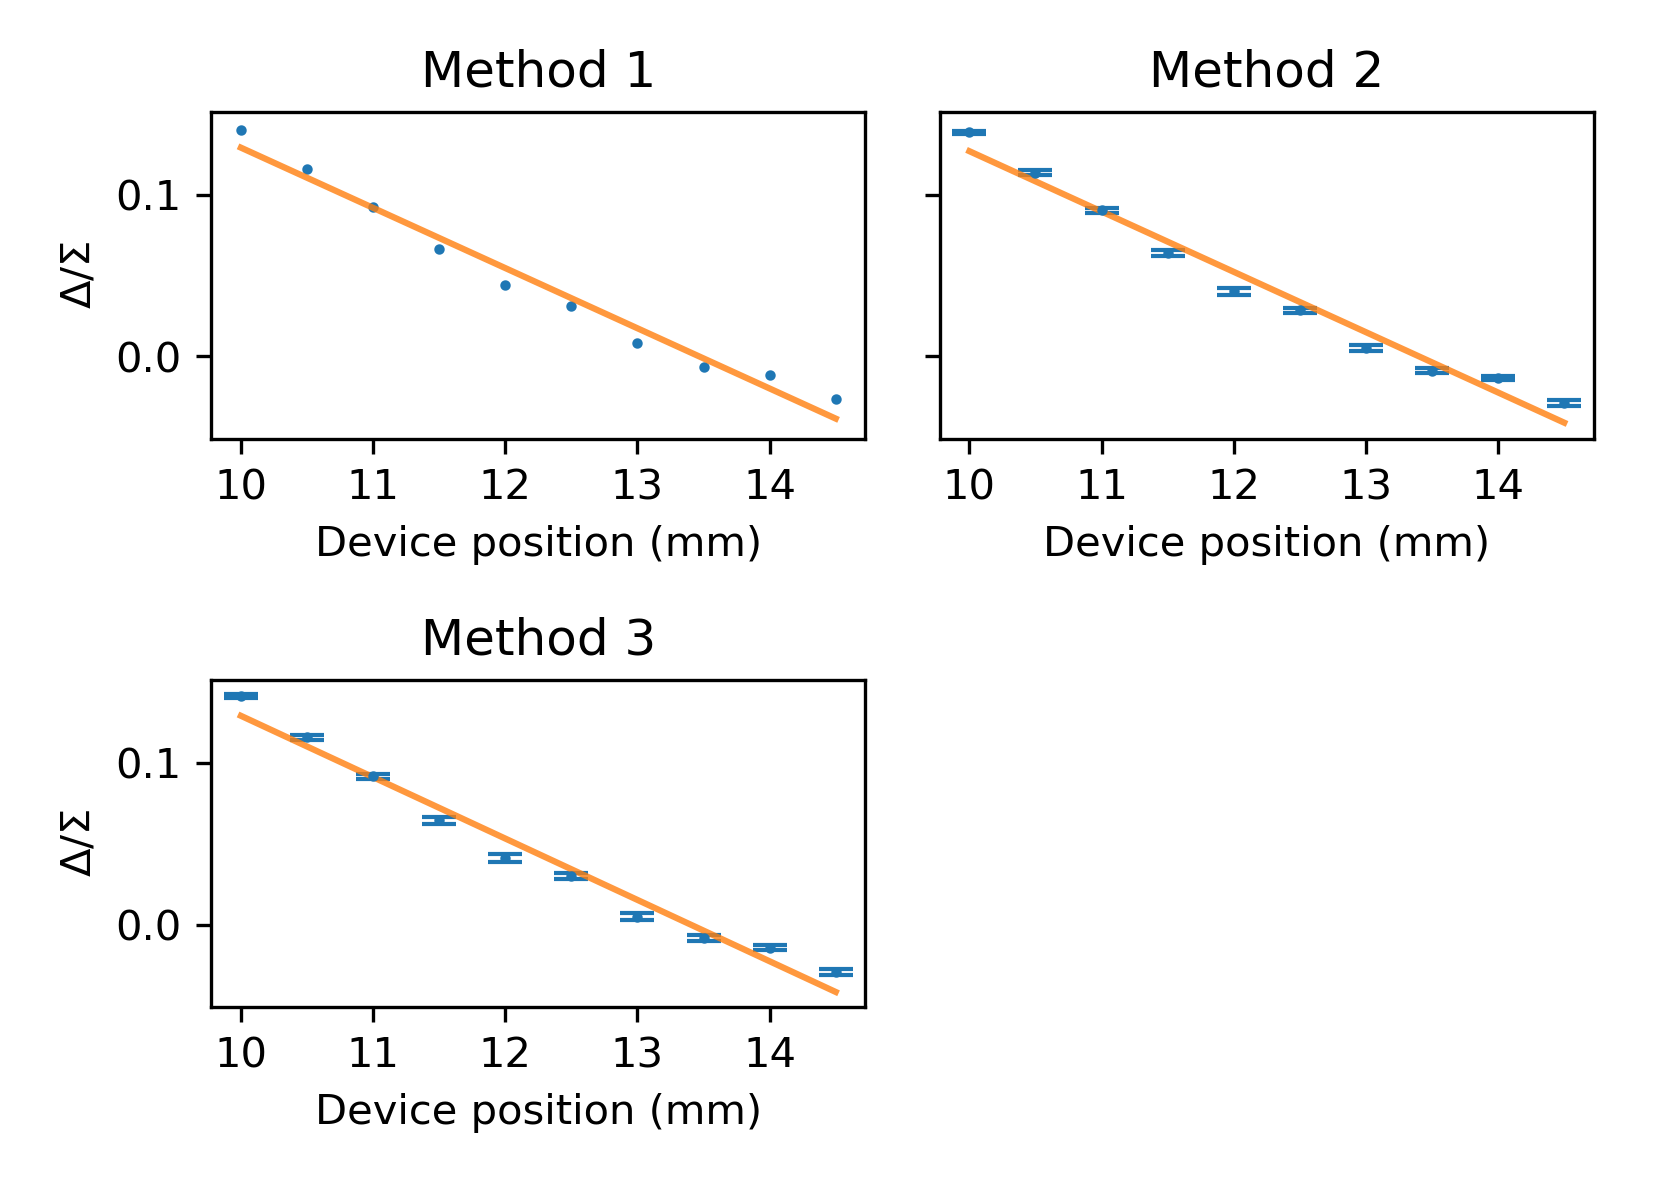
\includegraphics[scale=1, keepaspectratio]{pictures/fine_4_proc}
\caption{Comparison of the different processing methods together with the linear fit for the `fine scan' dataset. The fitting parameters are reported in Table~\ref{tab:fit_four_proc_1b}. The error bars represent the standard error of the mean of the response measured at each position.}
\label{fig:four_proc_1b}
\end{figure}


The same methods were applied to all available datasets, and the results are reported in Table~\ref{tab:fit_four_proc_1b}. As before, the methods are consistent within the same dataset. Figure~\ref{fig:all_dataset_1b_method2} shows the method 2 results for most datasets. The `coarse scan' dataset is not shown as over the large 25~mm range the response is not linear, as expected from theory. The $\Delta/\Sigma$ differences between the examined datasets can be explained by the device response not being properly linear in different position ranges. The linearity of the data fitted with a straight line are evaluated by mean of the reduced $\chi^2$. The reduced $\chi^2$ cannot be calculated for Method~1, as this method does not provide an uncertainty on the $\Delta/\Sigma$ values. Datasets acquired on reduced position ranges exhibit a good linearity, the most evident is the `$100~\mu$m scan' dataset that presents reduced $\chi^2$ of the order of 1 over a 1.5~mm range. Increasing the sampled position range to 2.5~mm, the `finest scan' dataset also exhibits a good linearity. In the 5~mm range, the non-linearity of the data points starts to become evident. The two datasets `fine scan' and `fine scan low charge' present a poor agreement to the linear fit, although the `fine scan low charge' features a visibly lower value of reduced $\chi^2$. 

\begin{table}[!t]
  \centering
    \begin{tabular}{c l c c c }
    \toprule
    Dataset & Parameter & Method 1 & Method 2 & Method 3   \\
    \midrule
    \multirow{4}{*}{fine scan}  & \multirow{2}{*}{\parbox{2cm}{Slope\\($\times10^{-2}$/mm)}}   & \multirow{2}{*}{$-3.7 \pm 0.2$} & \multirow{2}{*}{$-3.8 \pm 0.2$} & \multirow{2}{*}{$-3.9 \pm 0.2$}\\ 
    \\
                                & Intercept & $0.50 \pm 0.02$ & $0.51 \pm 0.02$  & $0.51 \pm 0.02$\\ 
    & $\chi^2$/DF & N/A & 35 & 29\\
    \hline\rule{0pt}{2.5ex}
    \multirow{4}{*}{finest scan}& \multirow{2}{*}{\parbox{2cm}{Slope\\($\times10^{-2}$/mm)}}    & \multirow{2}{*}{$-3.40 \pm 0.11$} & \multirow{2}{*}{$-3.42 \pm 0.12$} &  \multirow{2}{*}{$-3.45 \pm 0.11$}\\ 
    \\
                                & Intercept & $0.459 \pm 0.014$ & $0.458 \pm 0.015$ & $0.463 \pm 0.014$\\ 
    & $\chi^2$/DF & N/A & 3.6 & 2.7\\
    \hline\rule{0pt}{2.5ex}
    \multirow{4}{*}{\parbox{2cm}{\centering fine scan\\low charge}} & \multirow{2}{*}{\parbox{2cm}{Slope\\ ($\times10^{-2}$/mm) }}   & \multirow{2}{*}{$-3.4 \pm 0.3$} & \multirow{2}{*}{$-3.4 \pm 0.3$}  & \multirow{2}{*}{$-3.5 \pm 0.3$}\\ 
    \\
                      & Intercept & $0.45 \pm 0.04$ & $0.46 \pm 0.04$ &  $0.45 \pm 0.04$\\ 
    & $\chi^2$/DF & N/A & 6.0 & 6.1\\
    \hline\rule{0pt}{2.5ex}
    \multirow{4}{*}{\parbox{2cm}{\centering 100$\mu$m scan\\low charge}} & \multirow{2}{*}{\parbox{2cm}{Slope\\($\times10^{-2}$/mm)}}    & \multirow{2}{*}{$-4.67 \pm 0.19$} & \multirow{2}{*}{$-4.60 \pm 0.19$} & \multirow{2}{*}{$-4.15 \pm 0.15$}\\ 
    \\
                      & Intercept & $0.58 \pm 0.02$ & $0.57 \pm 0.02$ & $0.55 \pm 0.02$\\ 
    & $\chi^2$/DF & N/A & 1.23 & 0.98\\
    \bottomrule
    \end{tabular}
  \caption{Linear fit parameters for the three processing methods for most of the datasets. } \label{tab:fit_four_proc_1b}
\end{table}


\begin{figure}[!t] % figure and table in the same float

% \vspace{5mm}
\centering
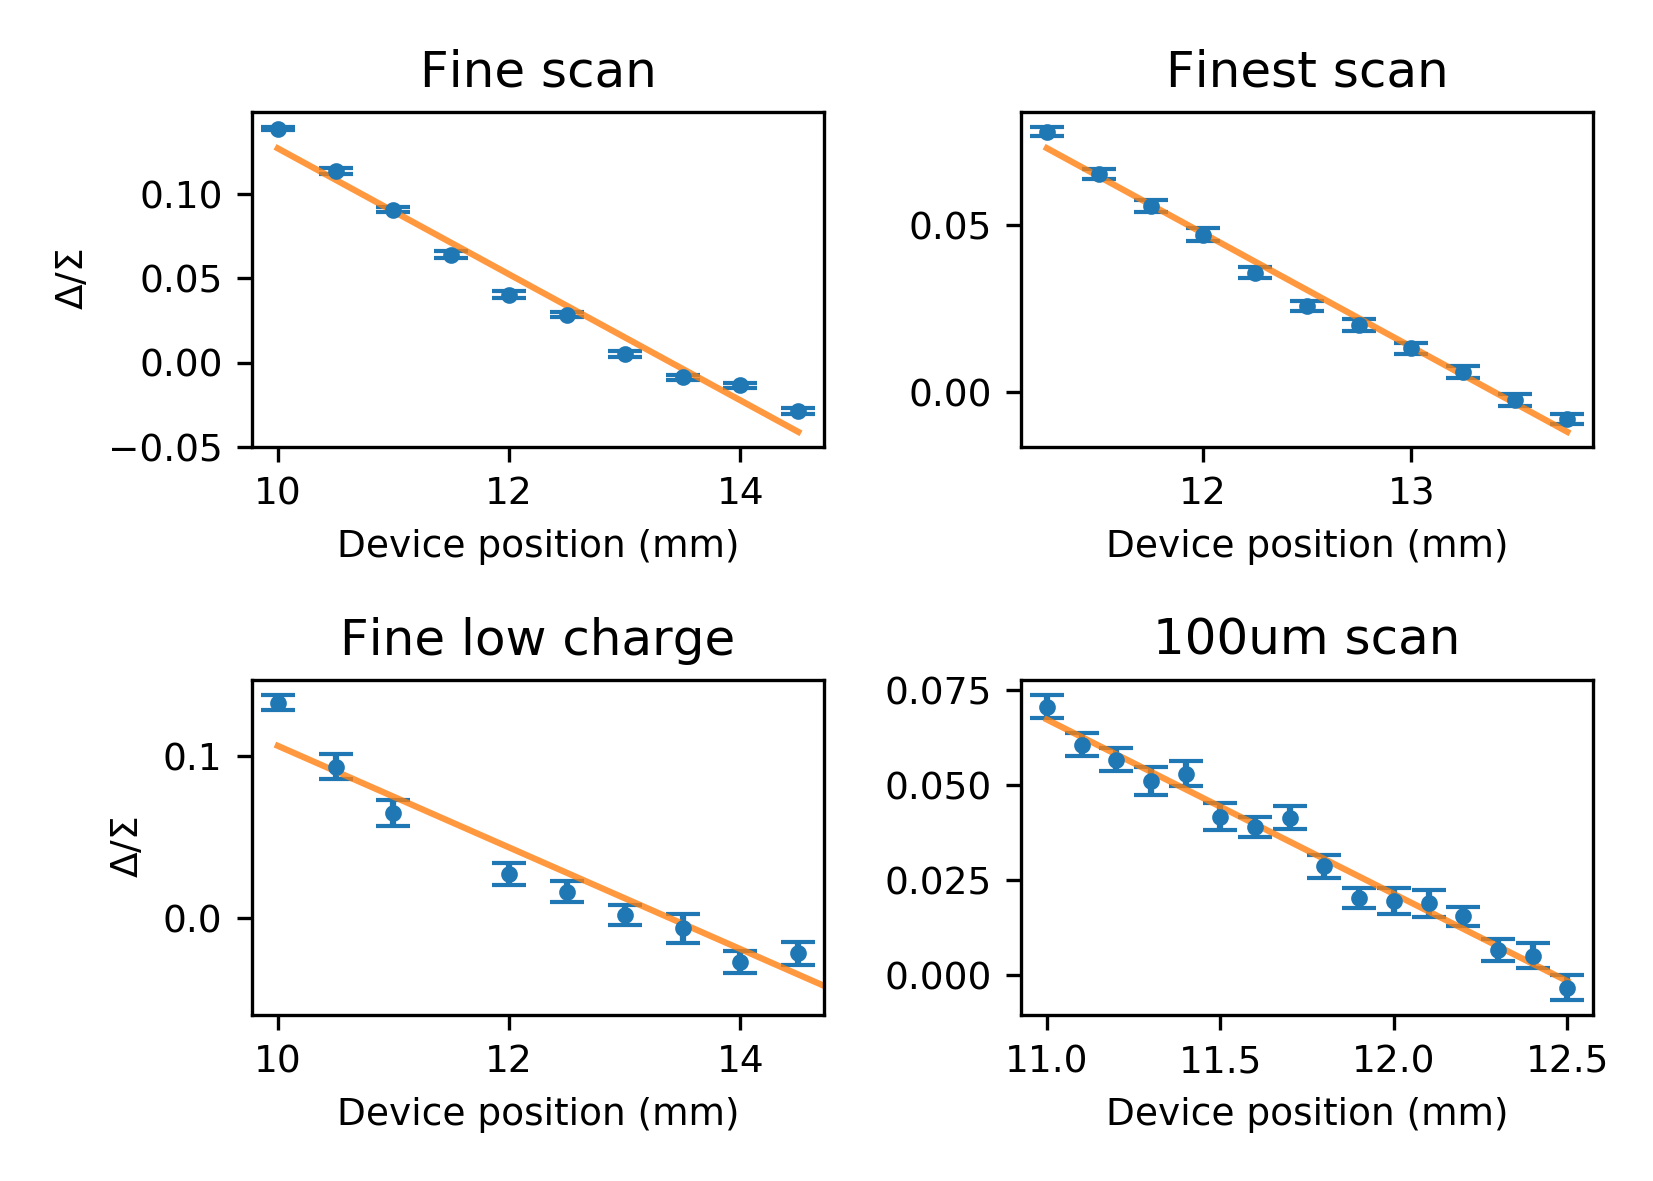
\includegraphics[scale=1, keepaspectratio]{pictures/4_dataset_method2}
\captionof{figure}{Each dataset processed with method 2}
\label{fig:all_dataset_1b_method2}
% \end{figure}
% \end{table}
% \newpage

% \begin{figure}[!b]
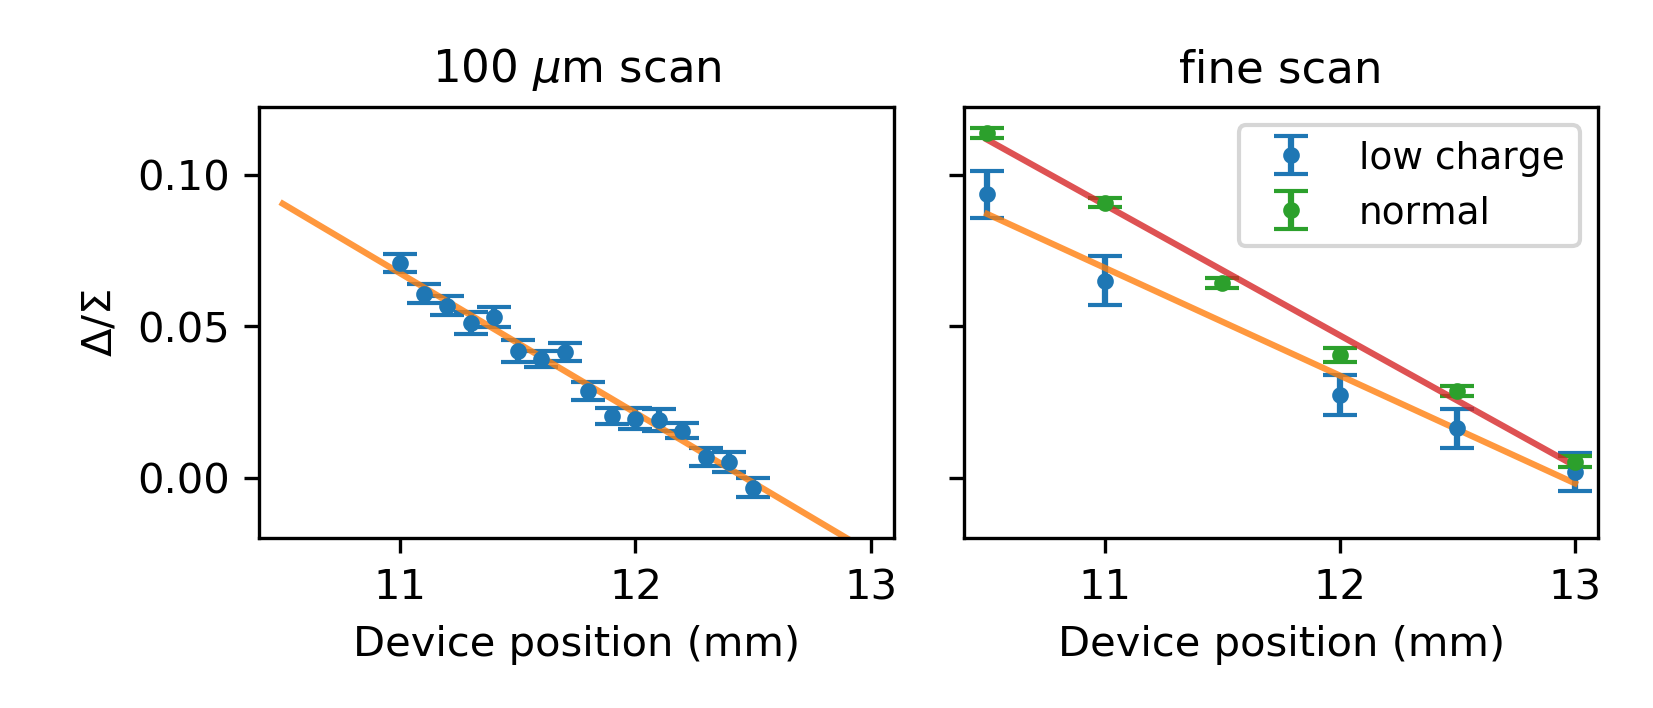
\includegraphics[scale=1, keepaspectratio]{pictures/comparison_100um}
\caption{Comparison of the $\Delta/\Sigma$ sensitivity calculated for the `$100 \mu m$ scan' dataset (left) and the `fine scan' and `fine scan low charge' (right) for the same translation stage position range. The error on the data in the `fine scan' dataset is visibly larger than in the others due to the reduced statistics. The fit parameters are reported in Table~\ref{tab:fit_small_range}.}\label{fig:comparison_100um}

% \vspace{4mm}
\end{figure}

\begin{figure}[!t]

  \centering
    \begin{tabular}{l c c c }
    \toprule
    Dataset & Slope $( \times 10^{-2} \text{ mm}^{-1})$ & Intercept  & $\chi^2$/DF \\
    \midrule
    $100\mu$m scan low charge    & $-4.6\pm0.19$ & $0.57\pm0.02$ &  1.2\\
    fine scan low charge & $-3.6\pm0.3$ & $0.46\pm0.04$ &  0.7\\
    fine scan          & $-4.30\pm0.18$ & $0.56\pm0.02$ &  5.1\\
    \bottomrule
    \end{tabular}
  \captionof{table}{Linear fit parameters for three datasets in the position range 10.5-13~mm.} \label{tab:fit_small_range}

\end{figure}

The dataset `100$\mu$m scan low charge' showed an average sensitivity up to 30\% larger than the other datasets. It was therefore compared to a subset of the other datasets over the same translation-stage position range. For all datasets, the $\Delta/\Sigma$ sensitivity increases when only the 11.0 to 12.5~mm translation-stage position range is analysed. Figure~\ref{fig:comparison_100um} shows how the results change for the full and reduced translation stage position ranges using the processing method~2 for two different datasets. To recalculate the fit, a shorter linear range was selected for the `fine scan' and `fine scan low charge' datasets. On the other hand, a range of 1.5~mm is too small for the `100 $\mu$m scan' dataset as it would use only three data points to estimate the two linear fit parameters. Instead, a range from 10.5 to 13~mm was used. Table~\ref{tab:fit_small_range} reports the linear fit parameters and the goodness of the fit is estimated using the reduced $\chi^2$ value. In both the subsets of the `fine scan' and `fine scan low charge'  datasets, the sensitivity to the beam position increased compared to the full position range and remain within 30\% difference also after considering the reduced datasets. 






In conclusion, the test device was demonstrated to be sensitive to the transverse beam position, but some non-linearity was observed. It must be emphasised that the test device was designed to allow maximum flexibility during the tests and that the acquisition chain was not optimised. Sources of non ideality of the measurements are: the alignment of the test device with the beam, the alignment of the detection system with the radiators, the beam-charge fluctuations that can drive the RF diodes to the non-linear regime in some shots. Furthermore, simulations show that the response of the test device is not linear outside a zone close to the centre (see Fig.~\ref{fig:sim_delta_sigma}), and the width of this region depends on the operation conditions of the RF diodes. 





\subsection[Response to beam position, for bunch trains]{Response to beam position, for bunch trains}\label{sec:5_bunch}

For particle beams formed of a train of bunches, the test device produces a number of RF pulses corresponding to the number of bunches in the train. Each pulse is detected by the Schottky diodes as shown in Fig.~\ref{fig:diode_signal_5b}. 

\begin{figure}[h]
\centering
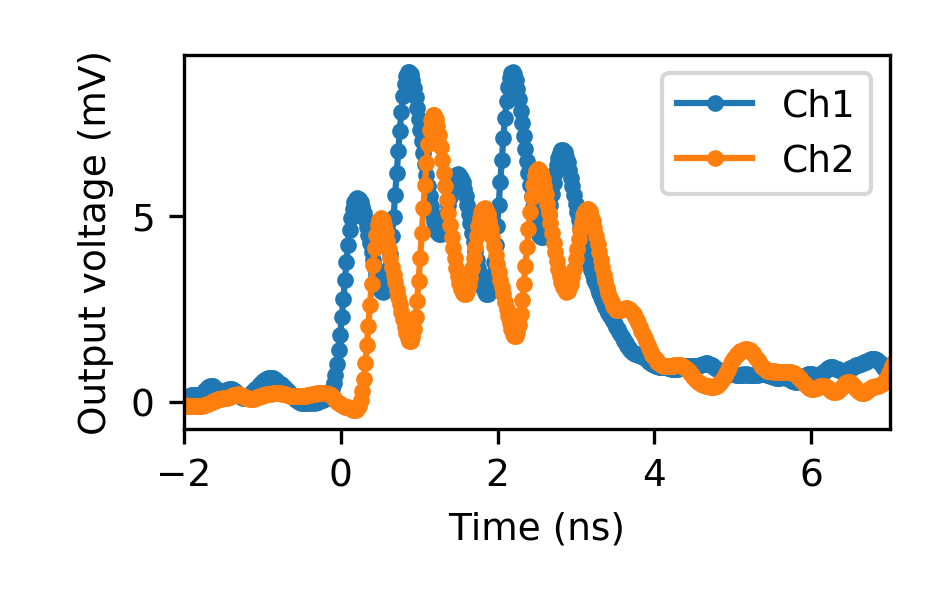
\includegraphics[width=10cm, keepaspectratio]{pictures/five_bunch_scope}
\caption{The signal produced by the Ka~band diode detectors for a train of 5 bunches. After the five peaks corresponding to the bunches spaced by 0.66~ns, a sixth smaller peak is visible at 3.8~ns. This is a smaller less intense bunch that is occasionally produced due to an imperfect setting of the CLEAR injector laser system.}
\label{fig:diode_signal_5b}
\end{figure}

When detecting bunch trains, the RF diode fall time is significantly longer than the bunch spacing. Therefore, the signal of the subsequent bunch is affected by the preceding one. The relative amount of signal leakage depends on the intensities of the ChDR emitted by both bunches. This aspect of Schottky-diode detectors will be discussed in Section~\ref{sec:diodes_leakage}. The source of the difference in the ChDR emission intensity of different bunches is the different charge or position of the bunches along the train. This effect, combined with the slow fall time of the RF diodes, determines the signal observed in Fig.~\ref{fig:diode_signal_5b}. Nevertheless, the three processing methods used for single-bunch beams can be applied to derive the average transverse position of the entire train. 

Two datasets were collected with trains of five bunches and parameters as listed in Table~\ref{tab:5bunch_test_param}.

\begin{table}[!h]
  \centering
    \begin{tabular}{l c c c}
    \toprule
    Dataset name & Train charge (pC) & Position scan range  \\
    \midrule
    fine scan    & $115\pm15$ & 4.5 mm\\
    finest scan  & $115\pm12$ & 2.5 mm\\
    \bottomrule
    \end{tabular}
  \caption{Parameters of the tests using trains of five bunches. The error on the train charge is the standard deviation.} \label{tab:5bunch_test_param}
\end{table}




\begin{figure}[!t] %both figures and table in the same floating environment
\centering
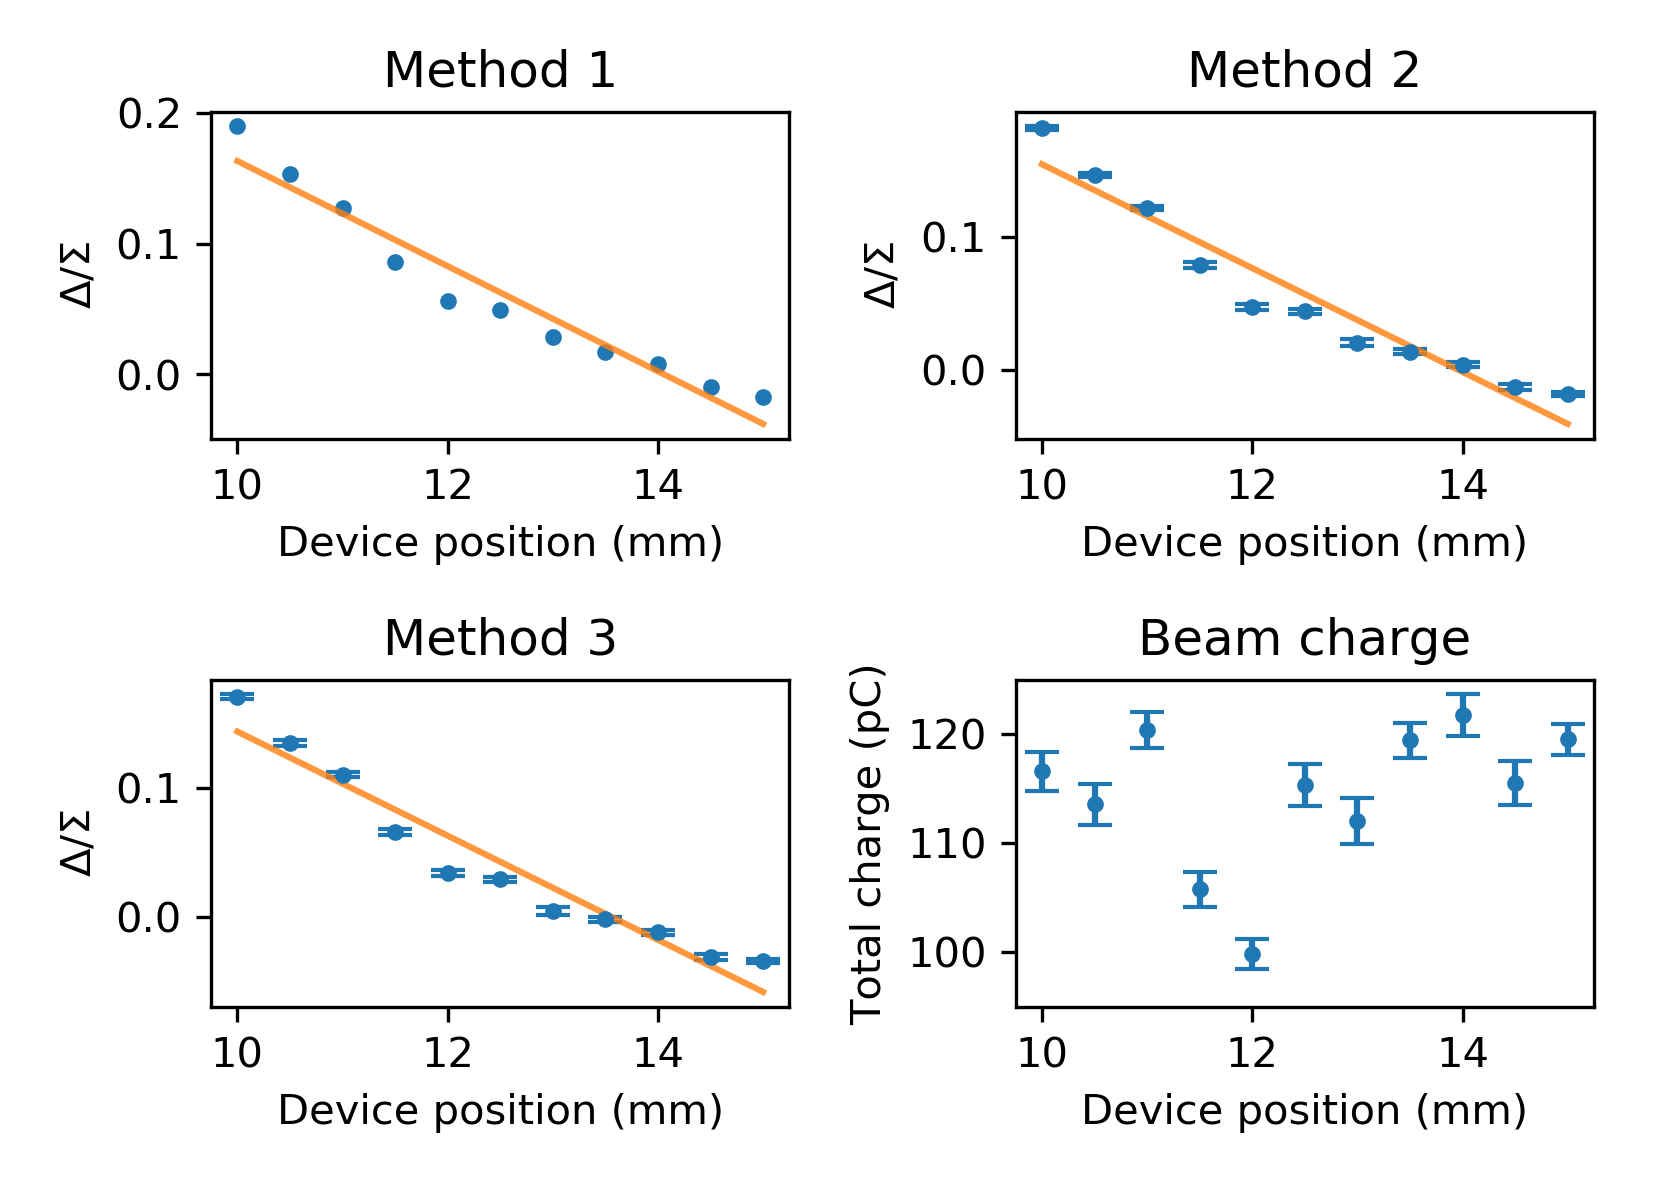
\includegraphics[scale=.8, keepaspectratio]{pictures/fine_4_proc_5b.png}
\caption{`Fine scan' dataset processed by the three methods.}\label{fig:5b_fine}



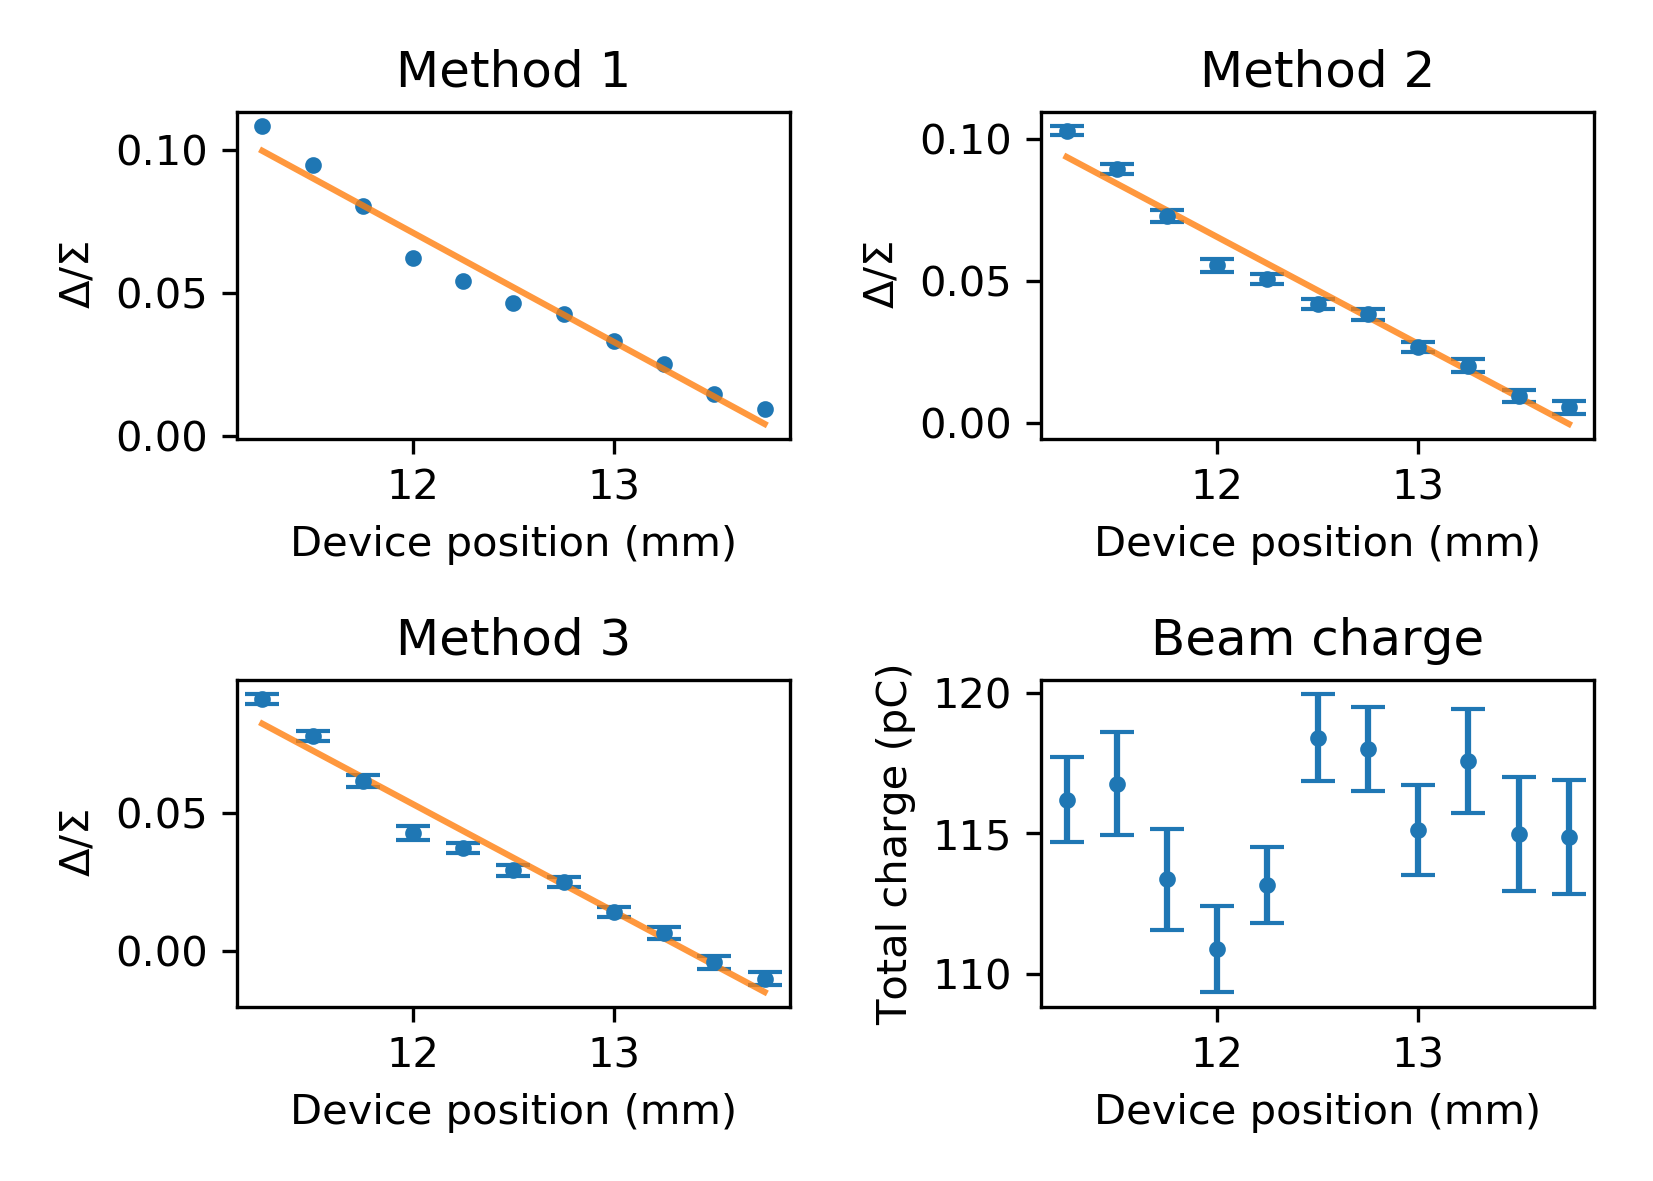
\includegraphics[scale=.8, keepaspectratio]{pictures/finest_4_proc_5b.png}
\caption{`Finest scan' dataset processed by the three methods.}\label{fig:5b_finest}
\end{figure}






% \begin{table}[!t]
\begin{figure}[!t]
  \centering
    \begin{tabular}{c l c c c }
    \toprule
    Dataset & Parameter & Method 1 & Method 2 & Method 3   \\
    \midrule
    \multirow{2}{*}{fine scan}  & Slope ($\times10^{-2}$/mm)    & $-4.0 \pm 0.3$ & $-4.0 \pm 0.3$ & $-4.0 \pm 0.3$\\ 
                                & Intercept & $0.57 \pm 0.04$ & $0.55 \pm 0.04$  & $0.56 \pm 0.05$\\ 
                                & $\chi^2$/DF & - & 101 & 83\\
                                \cline{2-5}\rule{0pt}{2.5ex}
    \multirow{2}{*}{finest scan}& Slope ($\times10^{-2}$/mm)    & $-3.8 \pm 0.2$ & $-3.9 \pm 0.2$ &  $-4.0 \pm 0.2$\\ 
                                & Intercept & $0.53 \pm 0.03$ & $0.56 \pm 0.03$ & $0.54 \pm 0.03$\\ 
                                & $\chi^2$/DF & - & 9.2 & 7.7\\
    \bottomrule
    \end{tabular}
  \captionof{table}{Linear fit parameters for the three processing methods applied to both datasets.} \label{tab:fit_four_proc_5b}
% \end{table}
% \end{figure}


\vspace{5mm}


% \centering
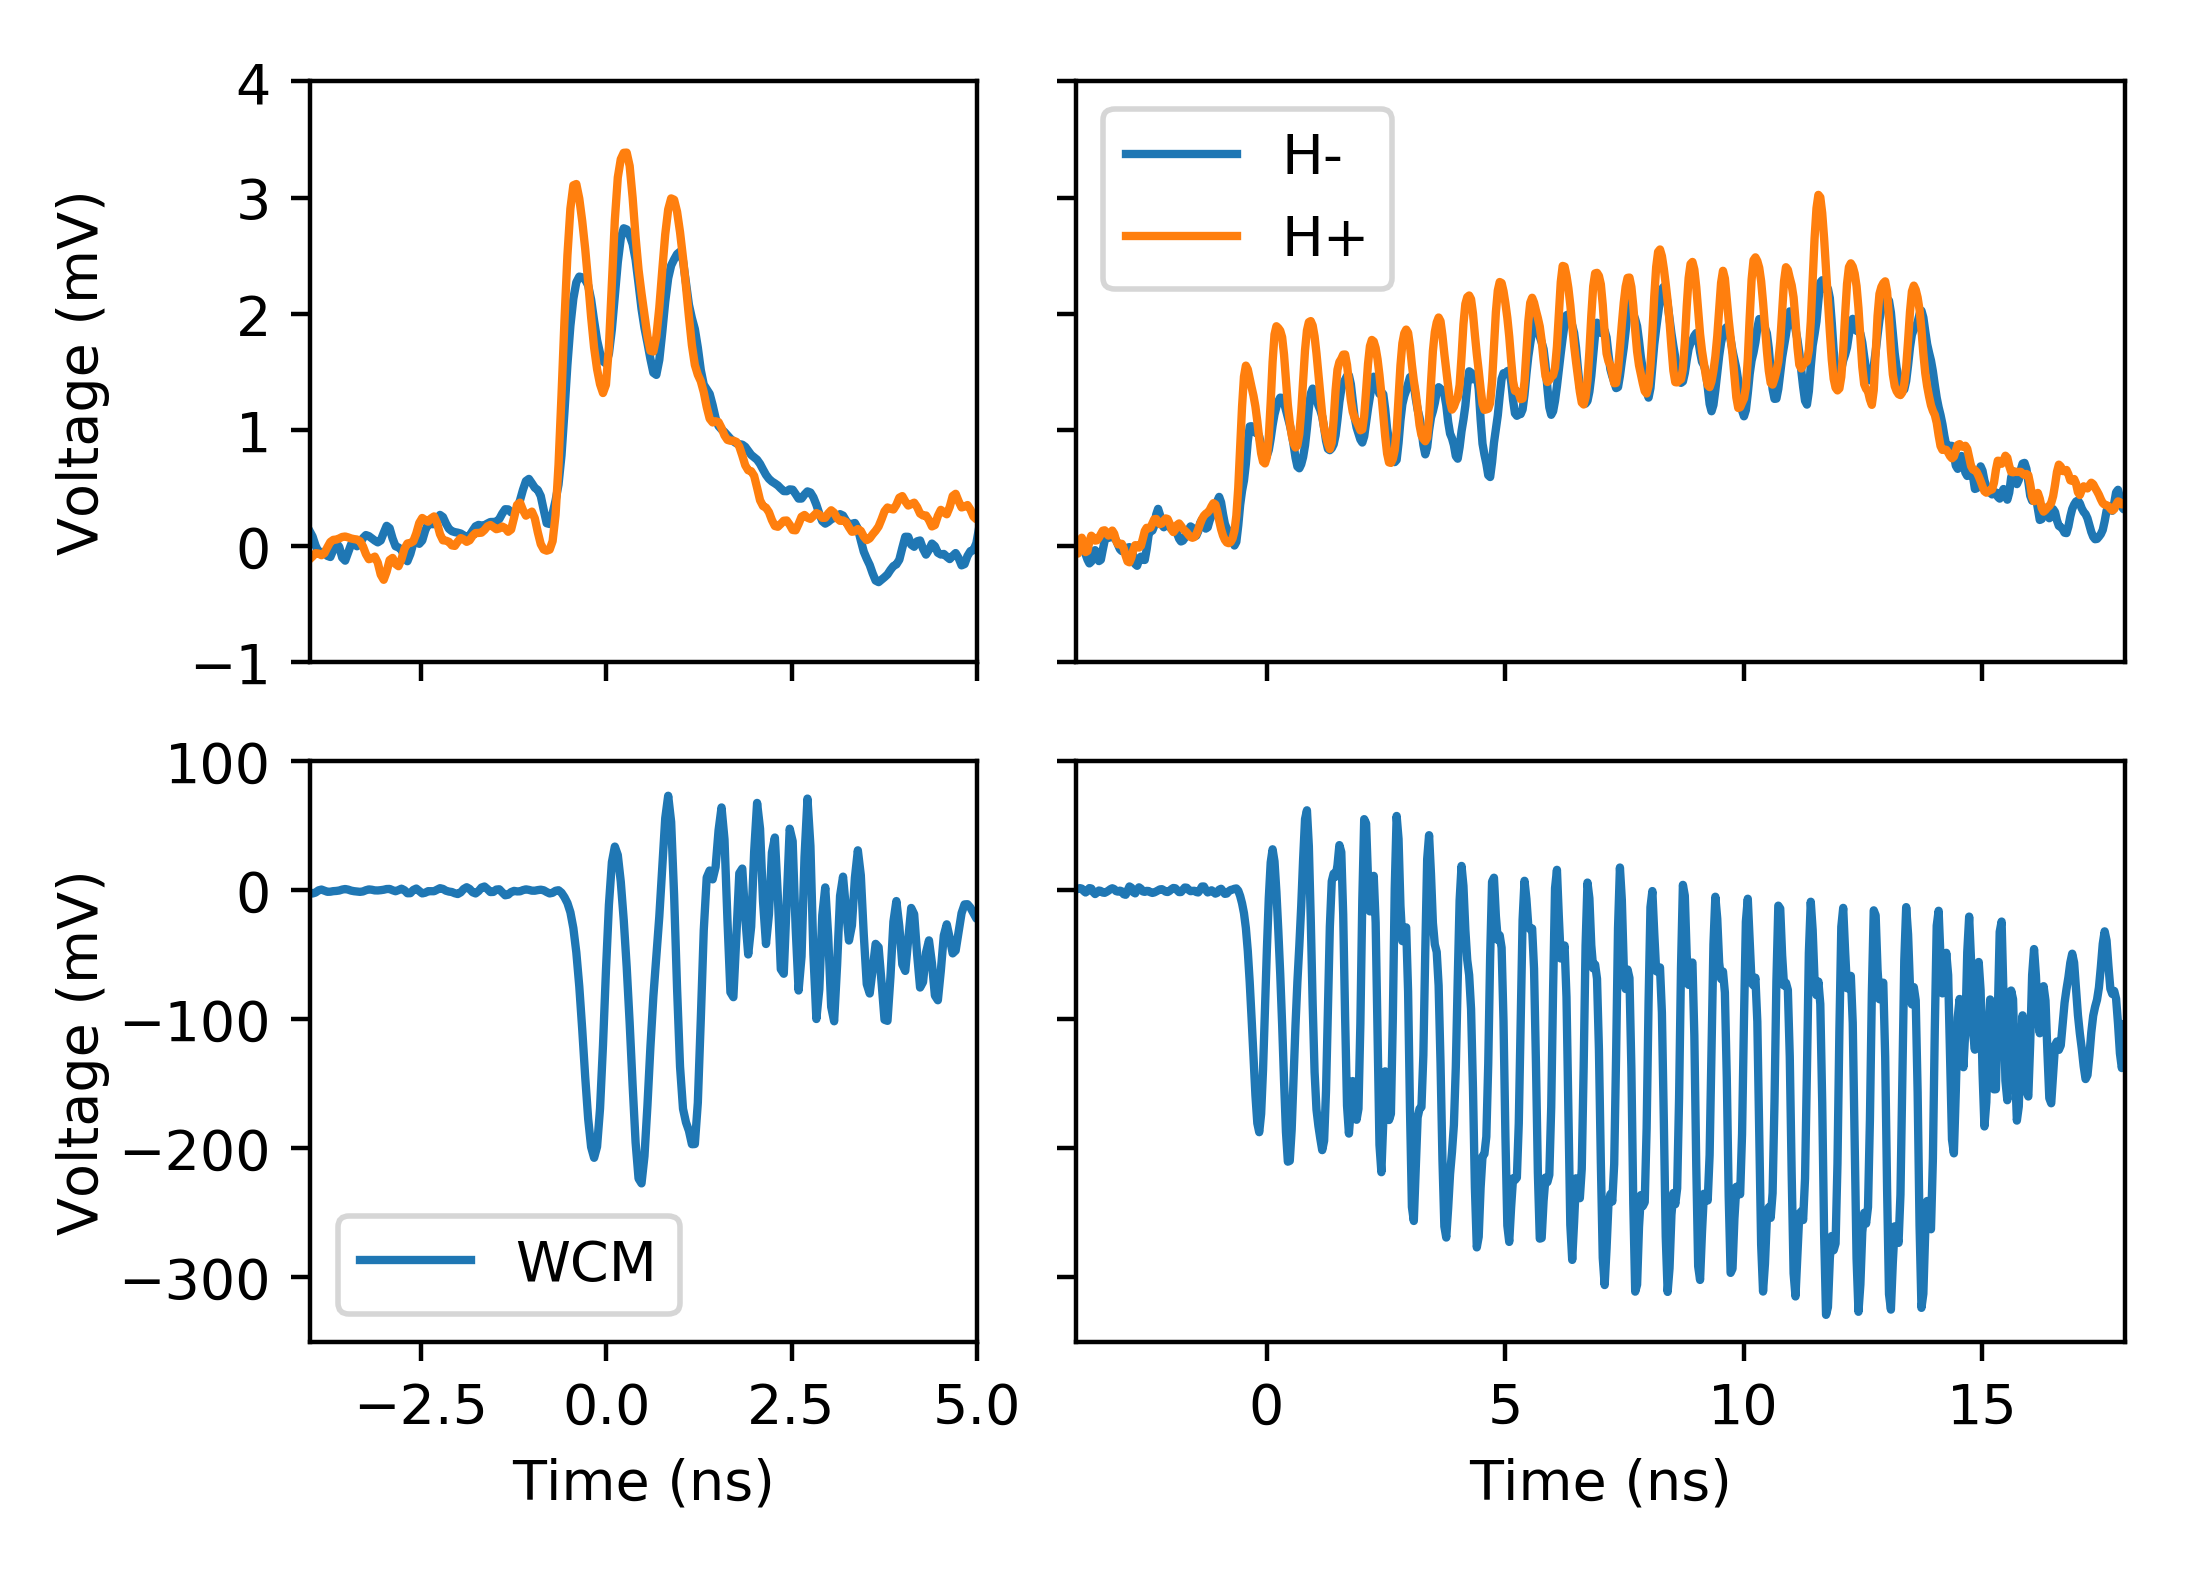
\includegraphics[scale=1, keepaspectratio]{pictures/ChDR-vs-WCM}
\captionof{figure}{ChDR signal from the diode detectors in the horizontal plane (top) compared to the Wall Current Monitor signal (bottom). The plots on the left show the measurements of a train of three bunches, while the plots on the right show the measurements of a train of 20 bunches. The signal level difference between both monitors is due to their design, attenuators and cables. The diode-detector signals show the emission in the Ka-band of the two PTFE radiators installed in the horizontal plane (H+ and H-). The amplifier baseline was not subtracted, and the gain is compensated.}
\label{fig:WCM}
\end{figure}


Figures~\ref{fig:5b_fine}~and~\ref{fig:5b_finest} show both datasets processed using the three different methods already used for single-bunch analysis. The linear fit parameters are reported in Table~\ref{tab:fit_four_proc_5b}. In both datasets, a non linearity is present at around the translation-stage position of 12~mm, but this is correlated with a momentary beam-charge reduction. It is possible that a temporary perturbation of the accelerator systems determined a beam production instability, that provokes a temporary charge reduction and energy modulation. This couples through dispersion, resulting in a beam displacement in the test stand. Such behaviour causes the calculated high values of reduced $\chi^2$. Despite the momentary drift during these measurements, the sensitivities in these tests are within 15\% of the response measured for single-bunch beams (see Table~\ref{tab:fit_four_proc_1b}).



The signal produced by the diodes installed on the ChDR test device was compared to the signal of the  Wall Current Monitor (WCM) installed upstream in the CLEAR beamline \cite{WCM-CLEAR}. The WCM is a high-bandwidth monitor designed to measure each bunch individually. One of the oscilloscope channels was connected directly to the WCM through a long coaxial cable while the remaining channels were used to observe the signals from the Ka-band system. The monitors are compared in Fig.~\ref{fig:WCM} for measurements of 3 and 20 bunches. The comparison shows that the detected bunch spacing is the same in both cases, and it is consistent with the CLEAR RF frequency. 

The WCM signal quality deteriorates after the first three bunches due to signal reflections and baseline drift caused by the bunch-to-bunch signal leakage that can be observed in longer trains (e.g. Fig.~\ref{fig:WCM}). However, the WCM has a faster fall time than the ChDR test device.

The comparison of the two instruments suggests that the bunched beam structure is correctly reproduced by the ChDR, but the fall time of the installed detection system is too slow to correctly distinguish individual bunches without polluting the signal of subsequent bunches. Therefore, the use of ChDR-based beam-position detection is valid for bunch-by-bunch position measurement, provided that a detection capable to resolve the different bunches is used.




\subsection{Limitations of the present setup  }\label{sec:diodes_leakage}

Schottky-diode-based RF detectors were chosen for this experiment for their flexibility and ease of use. Although they were successfully used in Section~\ref{sec:single_bunch} and~\ref{sec:5_bunch} to estimate the position dependence of the ChDR emission, they also highlighted some limitations such as their relatively slow fall time. No work describing the response of Schottky-diode detectors to short RF pulses has been found in the literature as not many applications use RF pulses of ps duration. Moreover, sources of such short pulses other than a particle beam are not widely available. For the work presented in this thesis, it is nevertheless interesting to discuss the diode response to a single-bunch beam and bunch trains. The data collected with the Ka-band diode detectors from the `fine scan' dataset introduced in Section~\ref{sec:single_bunch} were used to study the diode response.



\begin{figure}[!b]
\centering
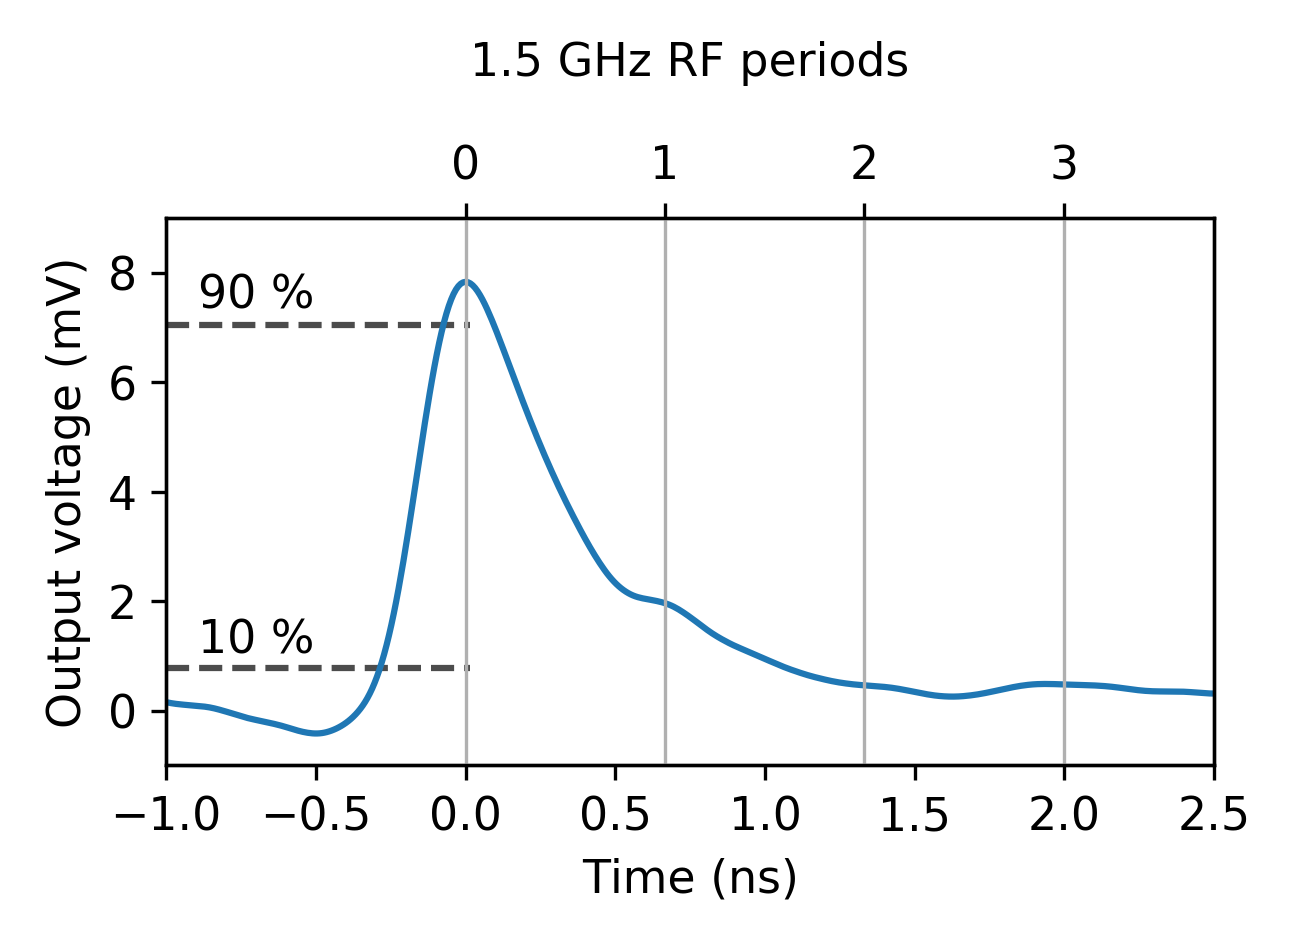
\includegraphics[scale=0.8, keepaspectratio]{pictures/Pulse_raise_fall}
\caption{Response of one of the Ka~band diode detectors to a single bunch. The RF periods of 666~ps are marked. In this acquisition, a shoulder is visible after one RF period. It is generated by the second, less populated bunch trailing the first one occurring due to an imperfect setting of the laser pulse picker system. The second bunch is not always present.}
\label{fig:diode_pulse}
\end{figure}

 Most RF detectors based on Schottky diodes exhibit a fall time significantly longer than their rise time. This is also the case for the RF detectors used in this experiment. The output voltage response to a single-bunch beam, and so to a single short RF pulse, is shown in Fig.~\ref{fig:diode_pulse}. 

The rise time of a signal is commonly defined as the time necessary for the output signal to move from the 10\% to 90\% of the peak output voltage. The average measured rise time of the Ka-band detectors was $0.20 \pm 0.05$~ns, with the uncertainty being the sampling time of the oscilloscope. The fall time is harder to measure precisely, due to the intermittent presence of a spurious bunch trailing the main bunch (see Fig.~\ref{fig:diode_pulse}). Neglecting this contribution the average fall time was $0.88 \pm 0.05$~ns.

It is possible that the real rise time was faster than measured, as the bandwidth of the complete acquisition system using long coaxial cables was neither measured nor corrected for. However, the fall time is longer than the accelerator RF period of 666~ps, resulting in signal leakage to the consequent bunches. The leakage affects mostly the next bunch. This is visible in Fig.~\ref{fig:diode_pulse}, where the RF periods, and so the position of any next bunch, is marked. Small drifts of the rise and fall times of the order of 5\% over 12 minutes were recorded, and can be attributed to thermal drifts~\cite{schottky_diodes_temp_extremes}. Detailed studies of the acquisition system for multi-bunch beams and of the RF diode response exceed the scope of this work.

A method to compensate the signal leakage between the bunches was tested, based on iterative subtraction of the leaking signal tail. Starting from the first bunch, its falling edge is fitted to a negative exponential function and then subtracted from the trailing bunches. After this compensation process, the real peak height can be estimated. Figure~\ref{fig:train_comp} shows the first iterations of this process. 




\begin{figure}[!t]
\centering
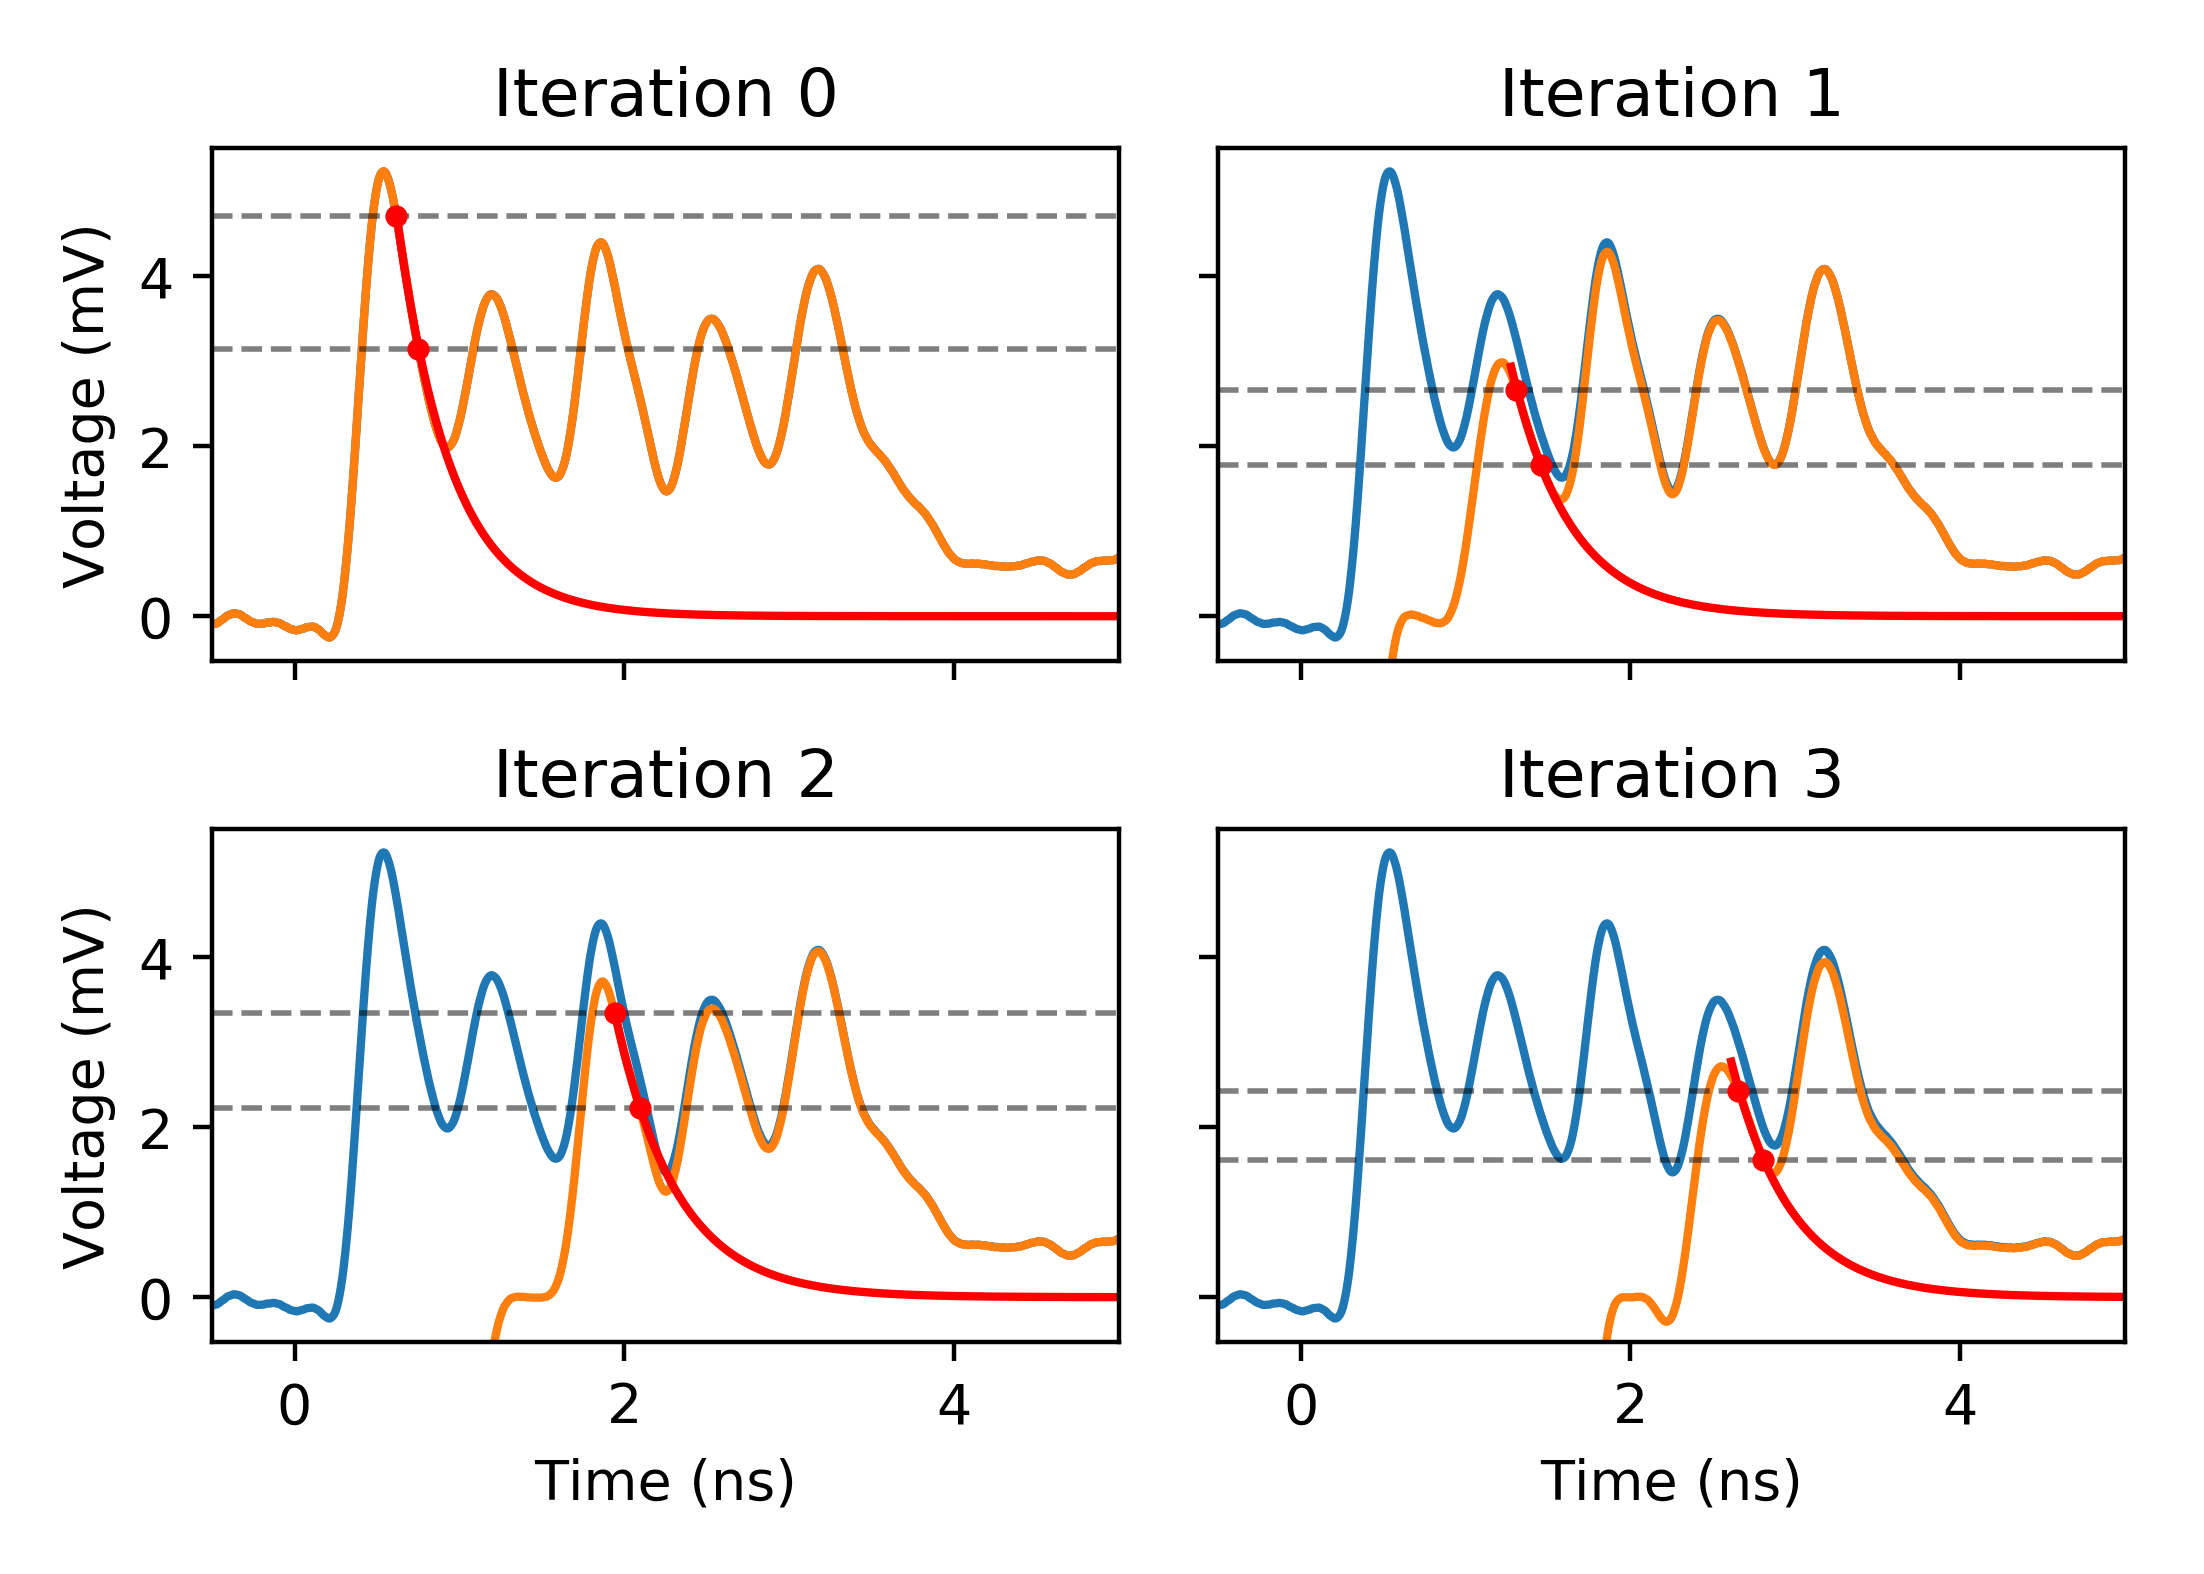
\includegraphics[scale=1, keepaspectratio]{pictures/train_compensation}
\caption{Successive iterations of the signal leakage compensation algorithm for a five bunch train. The blue trace shows the measured signal, the red one shows the negative exponential fit and the orange one shows the signal after subtracting the fit. The dashed horizontal lines delimit the fitted region, in this case between 90\% and 60\% of the peak voltage. At iteration 0 (top left), the blue and orange traces are overlapped, and the first peak is used for fitting the exponential decay. In iteration 1, the exponential decay fitted on the peak of the first bunch is subtracted from the signal, allowing to measure the correct height of the second peak (orange curve). The exponential decay is then fitted again onto the second peak after the correction, and it is used to move to the next iteration.}\label{fig:train_comp}
\end{figure}




Peak differences up to 85\% were present after the correction. These extreme cases correspond to two consecutive bunches with a large charge difference. In general, e.g. in the data shown in Fig.~\ref{fig:train_comp}, the leakage causes a wrong estimation of the peak height of the order of 20-30\%. However, the leakage is present in both diodes measuring opposite sides of the same plane and therefore its impact on the overall sensitivity is limited. Furthermore, this approach assumes that the RF diodes are linear to subtract the contribution of different bunches. This assumption might not always be correct. 
 

In the presence of very long trains, another anomalous behaviour of the RF diodes was detected. A series of measurements was performed using a beam consisting of 80~bunches, scanning the beam position over a 5~mm range. The output voltage level of the RF diode is rather constant along the bunch train, and the output voltage does not suggest any saturation (see Fig.~\ref{fig:saturation_signals}). 

\begin{figure}[!t]
\centering
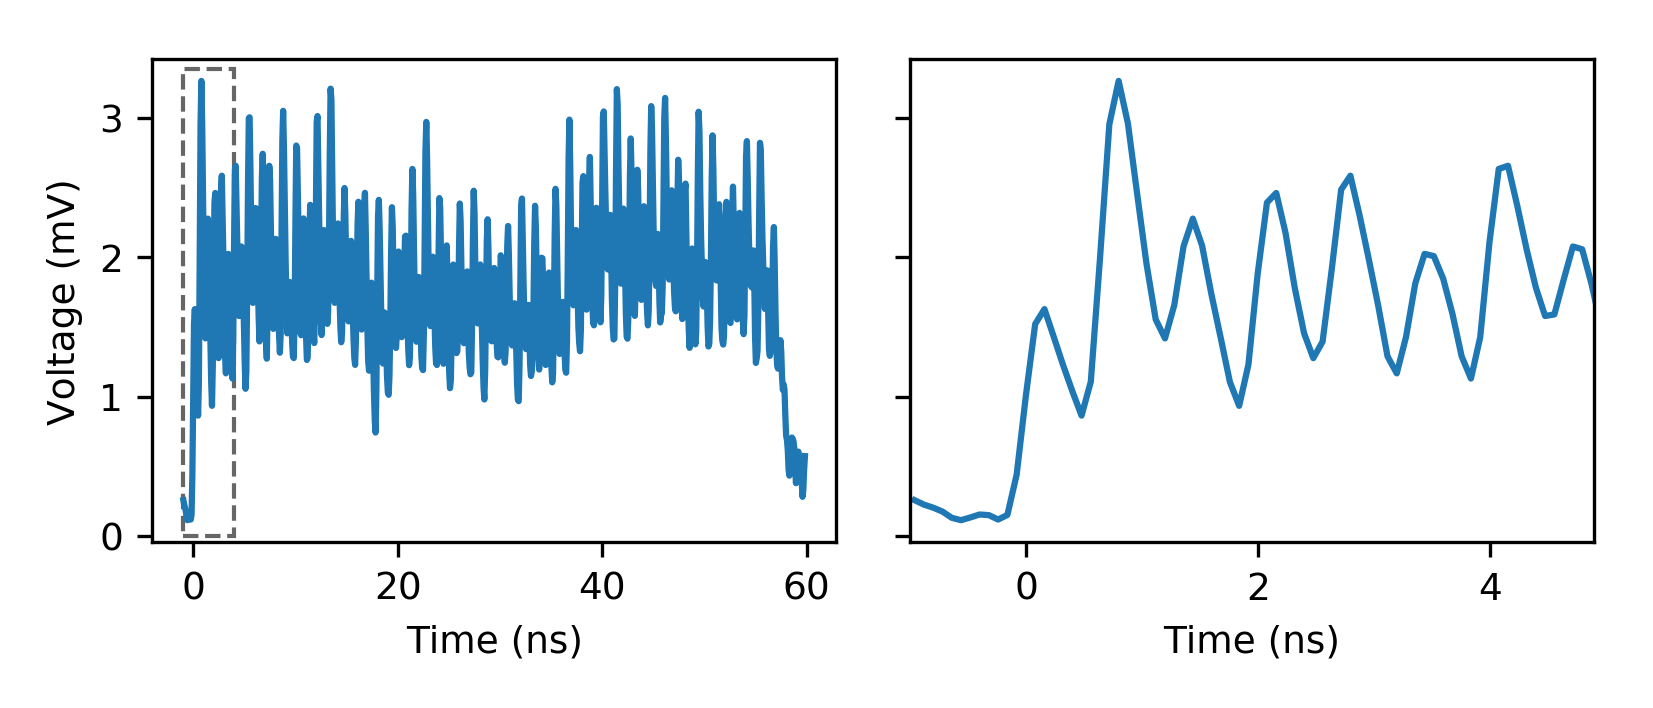
\includegraphics[scale=1, keepaspectratio]{pictures/long_train_signal}
\caption{Recorded signal of a Ka~band RF diode generated by a beam of 80~bunches. On the left the full signal is shown, while the region in the dashed box is presented on the right. }\label{fig:saturation_signals}

\vspace{3mm}
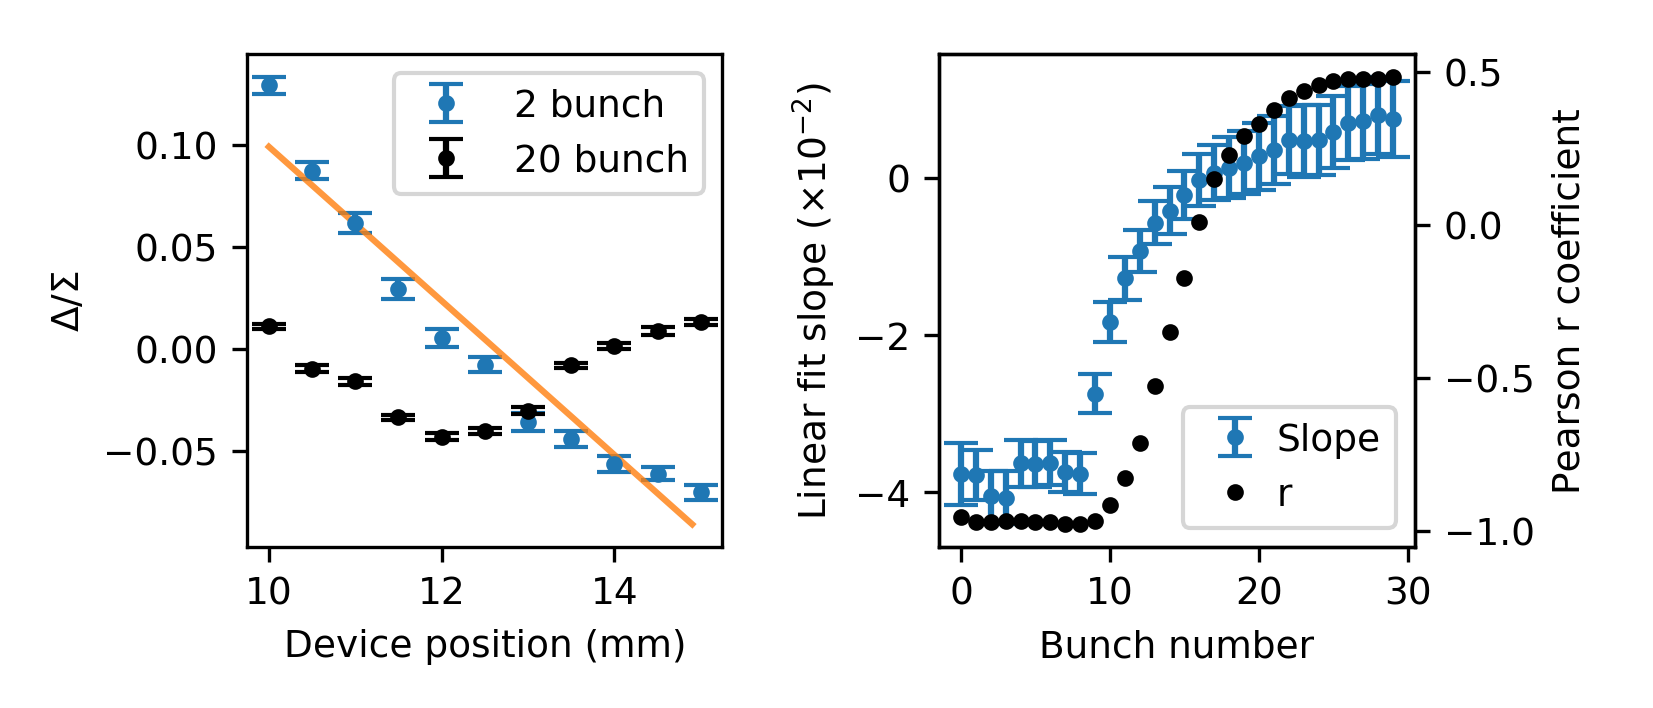
\includegraphics[scale=1, keepaspectratio]{pictures/long_train_response}
\caption{On the left, the beam position sensitivity measured for the first two and 20 bunches is shown. On the right, the slope of the linear fit and the Pearson r coefficient are presented as a function of the number of bunches considered.}
\label{fig:saturation_along_bunch}

\end{figure}

When computing the average train position with any of the three methods presented in Section~\ref{sec:single_bunch}, no position dependence is found. A more in-depth analysis windowing the diode signal to use only the first bunch, and then adding one bunch at a time in the train was carried out. The results of this analysis are shown in Fig.~\ref{fig:saturation_along_bunch}. On the left plot, the $\Delta/\Sigma$ curve is shown when considering only the first two bunches and the first 20. When only the first two bunches are considered, the response is linear. Conversely, when the first 20 bunches in the train are considered, the linearity and the position dependence are lost. The right plot of the figure shows a more systematic study of this behaviour. To estimate the linearity of the response the Pearson's r coefficient is plotted versus the number of considered bunches. The Pearson's r correlation coefficient is a statistical indicator with values between $-1$ and $+1$ \cite{stat:paper}, where the $\pm1$ value indicate perfect linearity while zero is the absence of linear correlation. The slope of the linear fit is reported as well, although it is not meaningful for nonlinear data. This analysis shows that after the first 10 bunches, the correlation between the diode output and the beam position is lost. For the moment, there is no clear explanation of this behaviour, and additional studies involving RF detectors of known internal structure would be needed to investigate it further. These effects are also essentially undocumented in literature, as the population of users of these devices that detect trains of ps-long RF pulses is extremely limited. 












\subsection{Directivity}\label{sec:directivity}

\begin{figure}[!b]

\centering
\subfigure[Reversed device installed for testing]{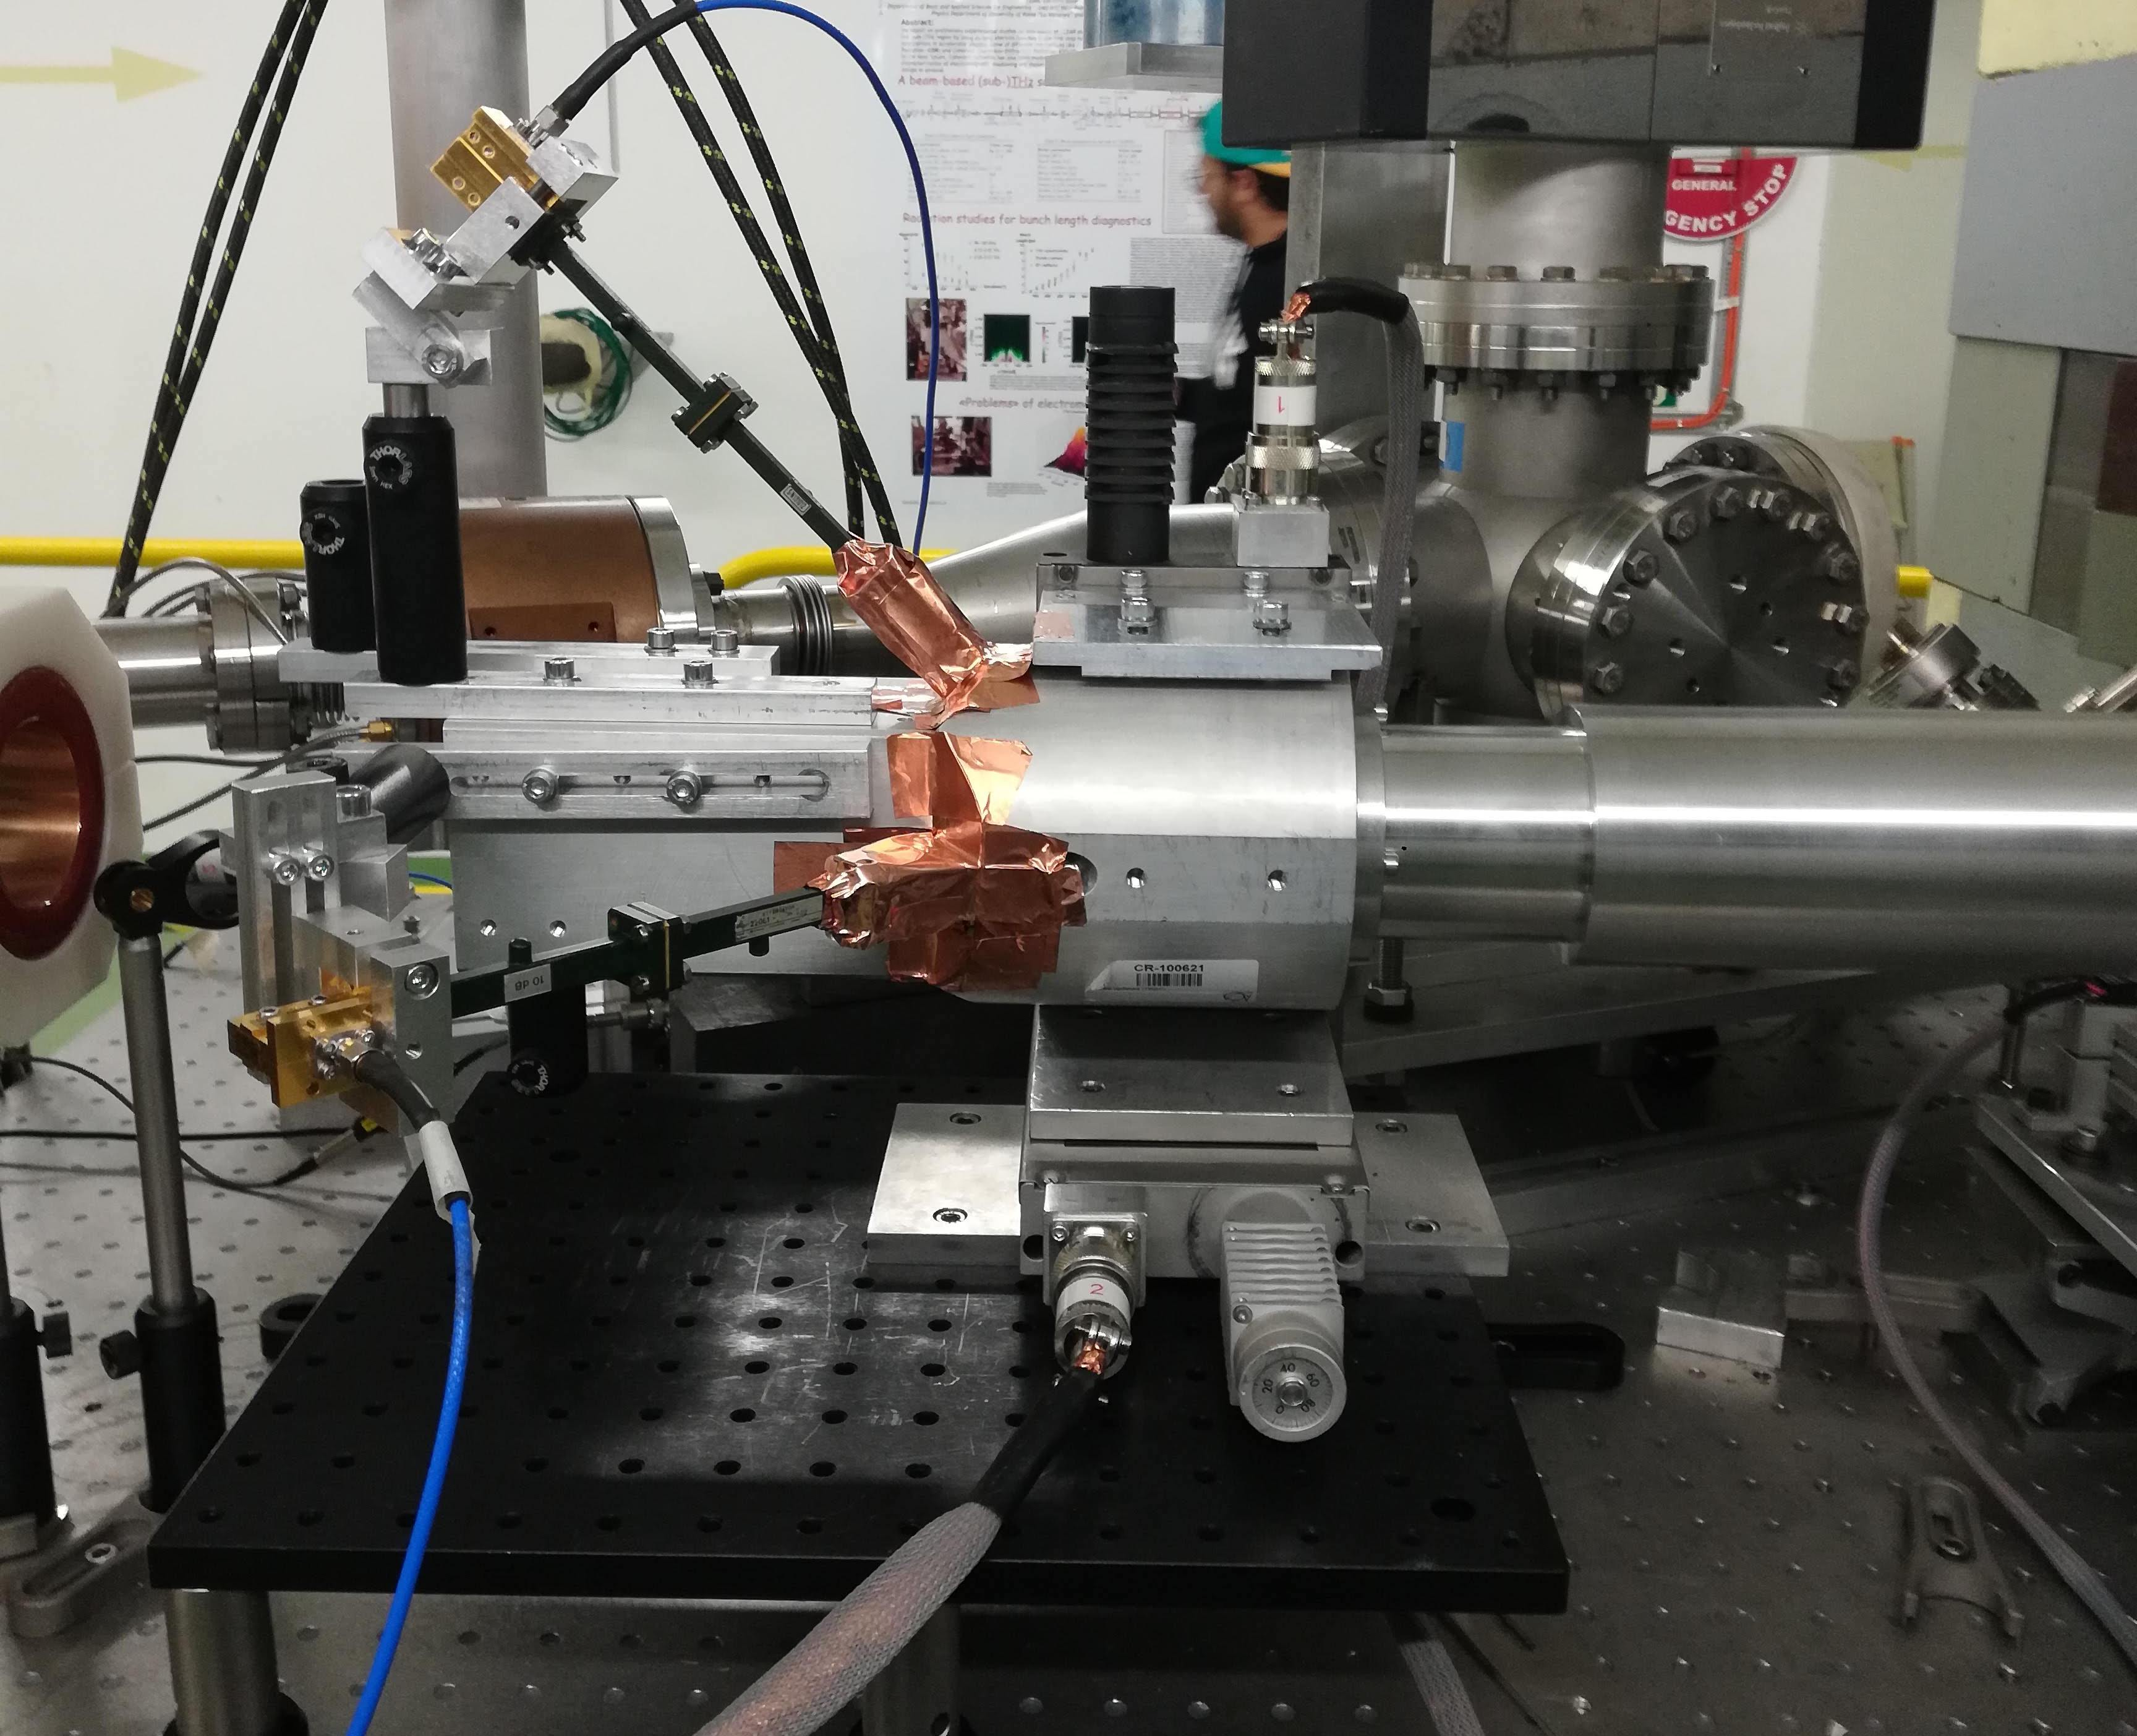
\includegraphics[width=6cm, keepaspectratio]{pictures/clear_reversed}}
\hspace{2mm}
\subfigure[Output signal]{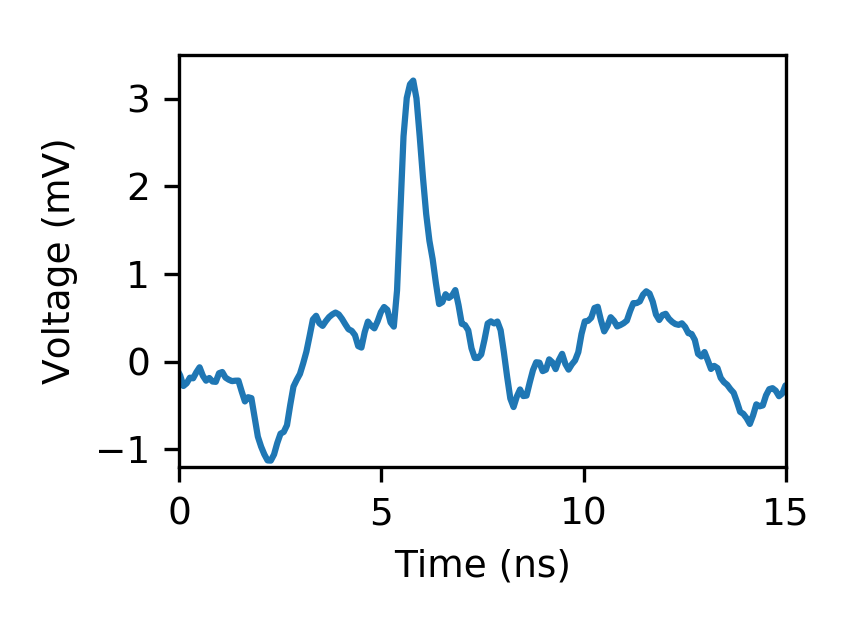
\includegraphics[scale=1, keepaspectratio]{pictures/scope_directivity}}
\caption{To test the directivity, the device was reversed as shown in (a). The beam is moving from left to right. The shielding copper foil connects the radiator output surfaces to the waveguide input of the detection system. Only one RF detector per plane was installed due to space constraints. The output signal of one of the RF detectors is shown in (b). The amplifier gain and baseline are compensated.}
\label{fig:reversed_bpm}
\end{figure}

Another interesting aspect when designing and testing a device of this kind is the directivity, i.e. the capability to selectively measure only the beam arriving from a given direction. In fact, the dielectric button BPM technology could be applied to any accelerator that features short bunches, including circular colliders. In such accelerators, two beams traverse the device in oppoite directions, and the signal generation in this case is investigated in this section.  The properties of the radiation produced by the beam passing in the forward direction were explained previously. To test the radiation production from the beam traversing the device in the backward direction, the device was rotated by $180^\circ$ about its vertical axis on the test stand. Figure~\ref{fig:reversed_bpm}~(a) shows the device after being reversed for this test. Only a single Ka-band diode detector was installed per plane. Due to the large number of electromagnetic reflections, produced mostly at the downstream beam dump, some copper foil was added for shielding the radiator and the RF detector. The diode detector output signal is shown in Fig.~\ref{fig:reversed_bpm}~(b). The immediate difference from the signal produced by the beam propagating in the forward direction (see e.g. Fig.~\ref{fig:diode_signal_1b} for comparison) is the presence of a rather large modulation of the baseline. This behaviour can be partially explained by the electromagnetic waves being reflected inside the copper foil due to its uneven section and shape. However, a part of this modulation is also generated by the ChDR emission itself and can be better understood through EM simulations. 









\begin{figure}[!t]
\centering
\subfigure[t $=380$ ps]{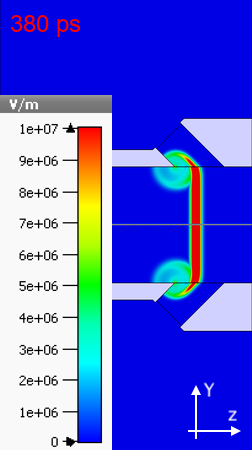
\includegraphics[width=4cm, keepaspectratio]{pictures/frame0_reverse}}
\hspace{2mm}
\subfigure[t $=450$ ps]{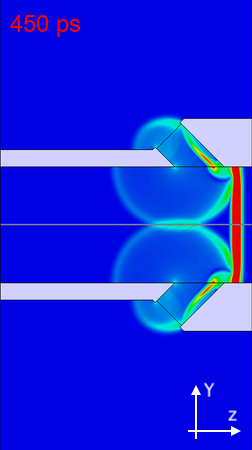
\includegraphics[width=4cm, keepaspectratio]{pictures/frame1_reverse}}
\hspace{2mm}
\subfigure[t $=490$ ps]{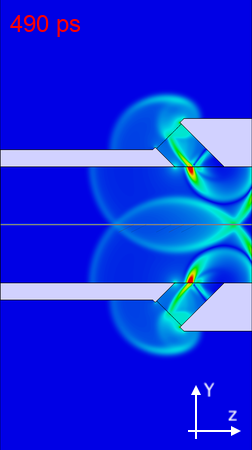
\includegraphics[width=4cm, keepaspectratio]{pictures/frame2_reverse}}\\

\subfigure[t $=550$ ps]{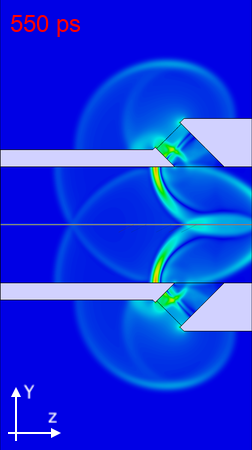
\includegraphics[width=4cm, keepaspectratio]{pictures/frame3_reverse}}
\hspace{2mm}
\subfigure[t $=600$ ps]{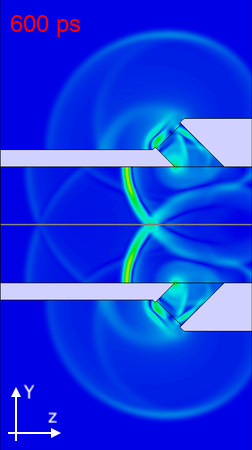
\includegraphics[width=4cm, keepaspectratio]{pictures/frame4_reverse}}
\hspace{2mm}
\subfigure[t $=650$ ps]{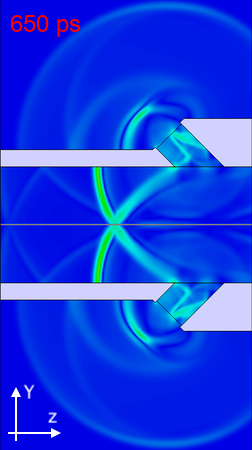
\includegraphics[width=4cm, keepaspectratio]{pictures/frame5_reverse}}

\caption{The absolute value of the electric field generated as the beam passes through the test device with reversed orientation. The ChDR front is generated when the beam arrives (a), but then it collides with the edge of the radiator and the metal that surrounds it (b). This results in a series of internal reflections on the metal walls, visible in (c), (d), (e). The various DR and ChDR fronts eventually exit the radiator surface with the strongest front clearly visible in (f). The results are generated with the single slice model, using the parameters: a simulation bandwidth of 50 GHz, 20 mesh cells per wavelength, 100 pC and 5 ps long electron beam.}
\label{fig:field_CLEAR_directivity}
\end{figure}


A simulation was carried out with the slice model presented in Section~\ref{sec:slice_model}. The results are presented in Fig.~\ref{fig:field_CLEAR_directivity}. The ChDR front is produced inside the radiator, but after travelling through the whole dielectric diameter it collides with the metal surface. The superposition of all internal reflections eventually escapes the radiator surface, together with the DR fronts that were generated, reflected and interfered inside the radiator. The emitted ChDR front is substantially more intense than the DR fronts that precede and trail it.

The tests revealed that, even with reverse orientation, the test device is emitting ChDR with reduced power and signal quality loss. Should this technology be used with the strict requirement of directivity, some major changes in the geometry need to be developed. The developed simulation model could be used to optimise the geometry and avoid the internal reflections. For example, developing a wedge-shaped radiator with two output surfaces.

















\newpage

\section[Tests with narrow-band diagnostics]{Tests with narrow-band diagnostics}\label{sec:narrowband-diagnostic}

Almost a year after the experiments described in Section~\ref{sec:test-in-air}, an additional measurement campaign was carried out to further study the use of ChDR for beam position measurement. 


\subsection{Experimental setup}

The test device was reinstalled in the CLEAR in-air test stand on a motorized support. In this testing campaign, emission from a single radiator was analysed. The device was displaced around the beam over a 20~mm range. The measurements were done with one of the vertical radiators due to the superior beam stability in that plane. Any drifts in beam energy or magnet settings were immediately visible in the horizontal plane as they were amplified through horizontal dispersion. The beam position was nevertheless constantly monitored with an OTR screen placed before the beam dump. The installed device is shown in Fig.~\ref{fig:clear_single_horn} and the detection system in Fig.~\ref{fig:clear_single_detection}.



\begin{figure}[!t]
\centering
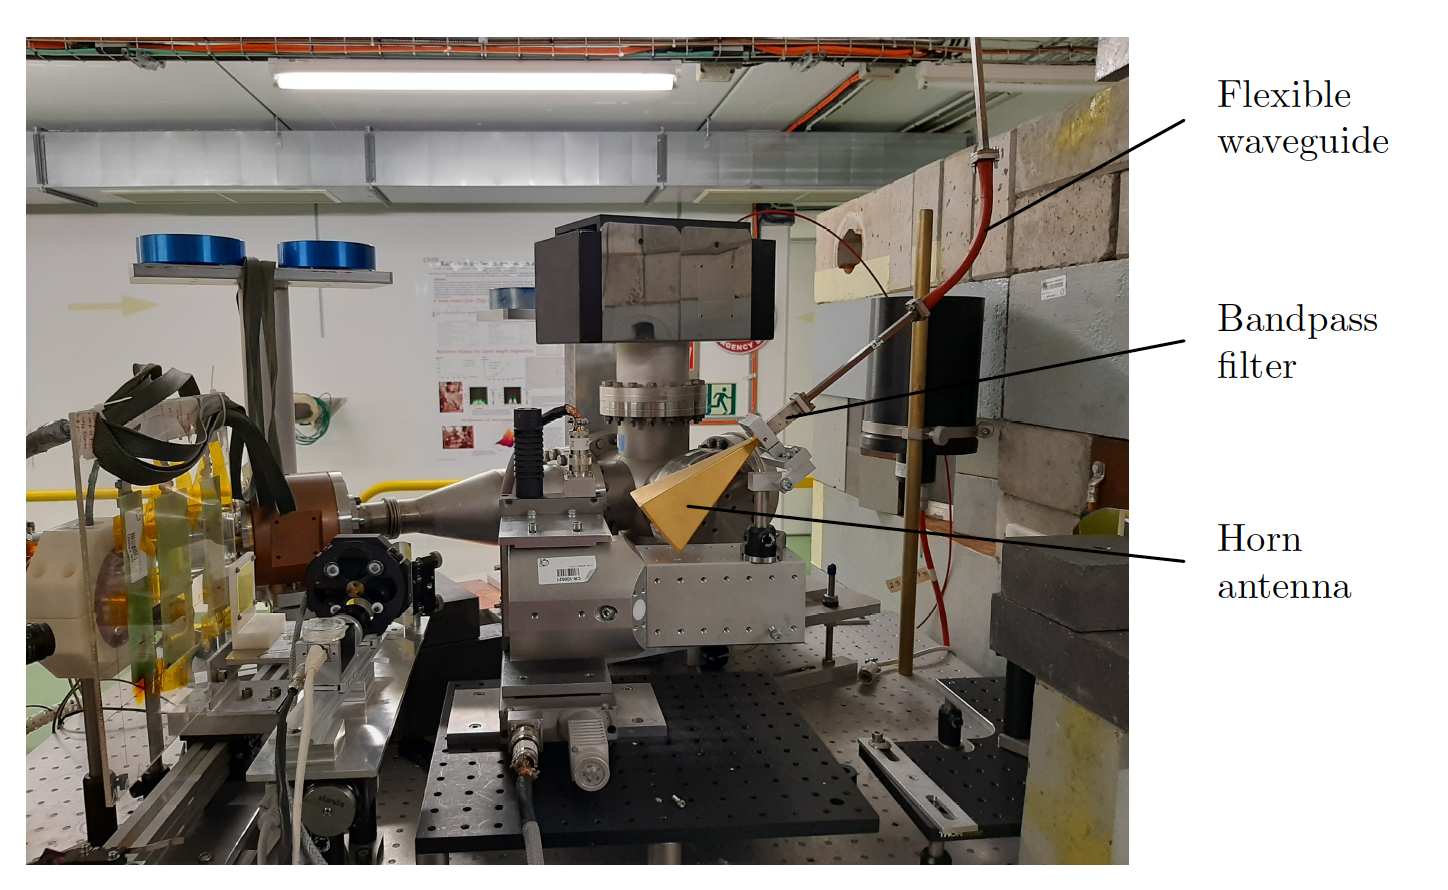
\includegraphics[width=13 cm, keepaspectratio]{pictures/setup-down-caption}
\caption{The test device reinstalled in the in-air test stand on movers visible in the centre. The beam exits the accelerator, going though the white Integrating Current Transformer on the left, traversing the test device and hitting the beam dump on the right. The radiator emission is captured by a horn antenna, and sent to the detection system through a waveguide network. }
\label{fig:clear_single_horn}

% \begin{figure}[!t]
% \centering
\hspace{40mm}
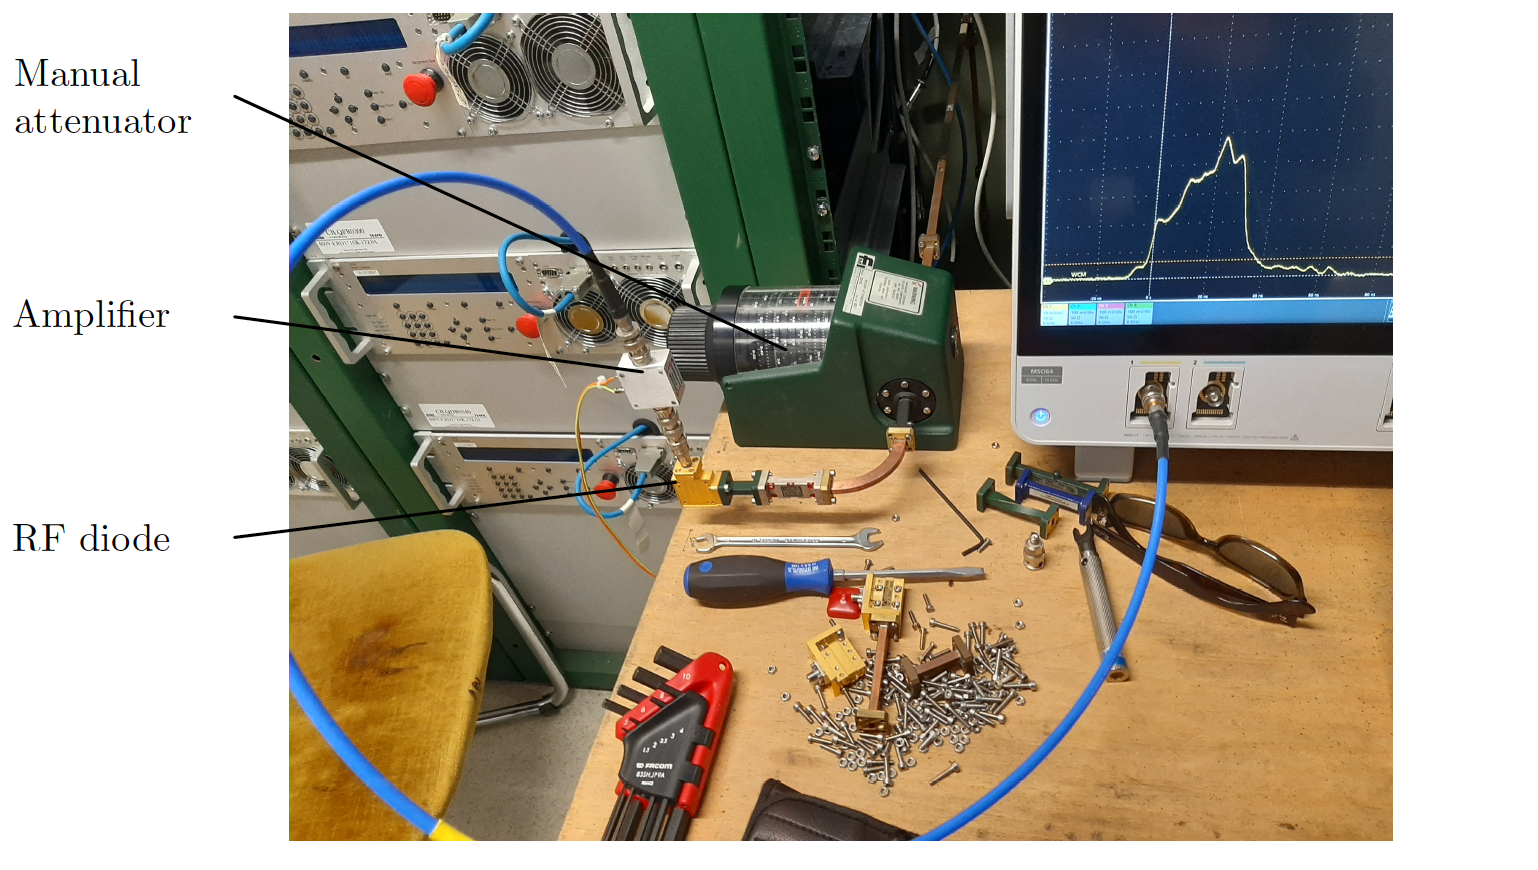
\includegraphics[width=14cm, keepaspectratio]{pictures/setup-up-caption}
\caption{The detection setup in the service gallery. The electromagnetic radiation arrives via the waveguide exiting the rack, then it proceeds to the rotary attenuator, finally reaching the RF diode. The signal is digitised with an oscilloscope after being amplified, if necessary.}
\label{fig:clear_single_detection}
\end{figure}

% \end{figure}

A large horn antenna in the Ka~band was installed in front of the radiator to couple the emitted signal to the detection system. A waveguide bandpass filter with a central frequency of 35.99~GHz and a passband of 1~GHz (model ELVA-1 BPF-28-35.99-1/20) connected the horn antenna to a waveguide network. The electromagnetic radiation was sent to the detector installed in a service gallery through a 15~m-long waveguide network. The filter proved to be necessary in preliminary tests to avoid deterioration of the broadband signal due to dispersion and reflections in the transmission chain. The waveguide network attenuated the signal by 11.5~dB. 

In the service gallery, a precision rotary manual attenuator was placed at the end of the waveguide network before the RF diode. The diode output signal was amplified, when needed, with a 28~dB, 500~MHz amplifier before digitization. 






The tests carried out with this setup present two main differences with respect to the tests described in Section~\ref{sec:test-in-air}:
\begin{enumerate}
    \item Propagation along the long dispersive waveguide stretches the pulse before it arrives at the RF diode.
    \item An attenuator in front of the RF diode makes it possible to maintain a constant input power. Therefore, the diode always works in the same region.
\end{enumerate}



\subsection{RF diode linearity}

The RF diode response was tested with single bunches and trains containing up to five bunches, since in such conditions it is possible obtain a good transport through the accelerator and maintain the same bunch charge in each bunch of the train. Each bunch carried a charge of 200~pC and had a length of 2~ps. 

In order to increase the radiated power, the test device was moved 20~mm off-centre with the beam passing 10~mm away from the radiator. The beam was maintained in a stable position during the measurements to obtain a constant ChDR production from the test device. The manual attenuator was adjusted in steps of 3~dB. For each setting, the average of 100~acquisitions was acquired 5 times. The averaging was carried out directly by the oscilloscope in order to reduce the noise. 


\begin{figure}[!b]
\centering
\hspace{40mm}
\includegraphics[scale=1, keepaspectratio]{pictures/bunch_number_vs_CW}
\caption{Diode output voltage as a function of the input power generated from ChDR (on the left), and from the CW synthesizer (on the right). The number of bunches is indicated in the legend. }
\label{fig:long_wg_linearity_scan}
\end{figure}

The measurement results are compared in Fig.~\ref{fig:long_wg_linearity_scan} to those obtained with the CW synthesizer set at 36~GHz, described in Section~\ref{sec:diodes}. First, it has to be noted that for a bunched beam no calibration of the absolute incident power is available. However, the attenuator settings allow for a correct relative scaling of the power between the different measured points. Secondly, for the ChDR generated by a bunched beam, two different operation regimes of the RF diode are reached. With a single bunch the diode remains in the transient regime, while for bunch trains of two or more bunches, the diode reaches the steady state regime. Hence, the measurements of a bunch train can be compared to those done with the CW synthesizer. The response exhibits the typical RF diode behaviour with the initial response linear with the input power which then becomes proportional to the square root of the input power. 



Assuming that the the bandpass filter and the waveguide network stretched the ChDR generated by bunch trains enough to reach the RF diode steady-state regime, the diode's response can be compared to the CW synthesizer measurements. This hypothesis is supported by the fact that the response does not change regardless of the bunch-train length. During the cross-calibration procedure, the response to 5 bunch trains was assumed equal to the CW response. This yields a factor of 5.58 to be applied to the arbitrary input power scale in Fig.~\ref{fig:long_wg_linearity_scan} to convert it to power in mW. Furthermore, this allows the diode response to be calibrated also for a single bunch. The cross-calibration results are shown in Fig.~\ref{fig:long_wg_linearity_scan_fit}. The sensitivities calculated for bunch trains of various lengths and CW are presented in Table~\ref{tab:fit_bunch_num_scan}. The sensitivity to short pulses produced by a  single bunch is $42.7\pm1.9$~mV/mW, i.e. less than half of that found for CW operation. 


\begin{figure}[!t]
\centering
\hspace{40mm}
\includegraphics[scale=1, keepaspectratio]{pictures/bunch_number_vs_CW_linear_region.png}
\caption{Diode output voltage for different levels of input power. The input power for bunched beam operation was deduced by  cross-calibration with the CW source in the linear operation region.}
\label{fig:long_wg_linearity_scan_fit}

% \vspace{2mm}
\end{figure}


\begin{figure}[!t]
\centering

\begin{tabular}{l c c c c c c}
\toprule
Number of bunches & Intercept (mV) & Slope (mV/mW)\\
\midrule
1 & $(-0.8\pm8.6)\times10^{-2}$ & $42.7\pm1.9$  \\
2 & $(2\pm39)\times10^{-2}$ & $104\pm8$  \\
3 & $(1.2\pm4.4)\times10^{-1}$ & $101\pm9$  \\
4 & $(2\pm34)\times10^{-2}$ & $103\pm7$  \\
5 & $(2\pm20)\times10^{-2}$ & $101.3\pm5.5$ \\
CW & $(-88\pm2)\times10^{-2}$ & $101.3\pm0.3$ \\
\bottomrule
\end{tabular}
\captionof{table}{Linear fit parameters for Fig.~\ref{fig:long_wg_linearity_scan_fit}. The slope is RF diode sensitivity under various test parameters.} \label{tab:fit_bunch_num_scan}

\end{figure}






\subsection{Response to beam charge}

\begin{figure}[!t]
\centering
\hspace{40mm}
\includegraphics[scale=1, keepaspectratio]{pictures/Charge_scan}
\caption{Left, measured emitted power depending on the single bunch charge. The fit with the quadratic curve is shown, representing the expected dependence for coherent radiation. The emitted power is measured by attenuating the input signal on the diode by a known factor, in order to keep a constant output voltage of 1.5~mV. This procedure ensures that the diode does not change the operation regime. The measured diode output voltage (in blue) and the manual attenuation settings (in red) are reported in the plot on the right-hand side.}
\label{fig:charge_scan_single_wg}
\end{figure} 

The test device response to a single bunch was measured in the charge range between 3 and 525~pC. The result of the measurement is shown in the left plot of Fig.~\ref{fig:charge_scan_single_wg}. The goal was to perform the measurement of the emitted power while keeping the diode detector working in a constant regime. To make sure that the diode works constantly in the same regime, the input power is reduced by mean of the attenuator, maintaining the output voltage at 1.5~mV. The radiated power can then be reconstructed by means of the diode output voltage and the attenuator setting. Constant output voltage was measured for bunch charges above 40~pC, as shown in the right-hand side of Fig.~\ref{fig:charge_scan_single_wg}. For smaller bunch charges, the attenuator was set to zero, and the full radiated power was delivered to the diode. 

The measured power production was fitted to a quadratic function ${P = a \, q^2}$, where $q$ is the beam charge, as it is expected for coherent radiation production in Equation~\ref{eq:coh-rad}. The obtained fit parameter is ${(4.11\pm0.12)\times10^{-5} \text{ mW/pC}}$. The quadratic dependence is valid only for data points recorded with a charge below 400~pC. Above this charge, a saturation of the power production is recorded. It can be excluded that the saturation is related to the experimental setup as the beam position was stable and the input power on the diode was kept in the same regime also at charges above 400~pC. Conversely, it is likely that the charge increase caused a bunch elongation \cite{Thibaut_pc} which reduces the beam spectral power at high frequencies and therefore reduces ChDR production in the detected band. Unfortunately, no measurements of the bunch length were available for this dataset. 





\subsection{Response to beam position}

Using the same procedure as for the charge scan, the vertical position of the test device was also varied while controlling the RF diode input power with an attenuator. The explored displacement from the beampipe centre ranged between -0.25 and 20.75~mm. The radiated power as a function of the beam position is shown in the left plot of Fig.~\Ref{fig:position_scan_single_wg}. The recorded beam charge, the diode output voltage and the attenuator settings are shown in the right plot of the same figure. 



\begin{figure}[!b]
\centering
\includegraphics[scale=1, keepaspectratio]{pictures/Position_scan}
\caption{Left, measured radiated power as function of the beam position. The distance from the radiator is also reported on the top axis. An exponential fit is shown. Right, the experiment parameter for each data point. For each position, the charge (in blue), the diode output voltage (in black) and the attenuator settings (red solid line) are reported.}
\label{fig:position_scan_single_wg}
\end{figure}

The measured data can be used to derive the beam position sensitivity of the test device. By fitting the data to an exponential function, the response of a second detection system for the opposite electrode can be extrapolated. The derived sensitivity is shown in Fig.~\ref{fig:delta_sigma_single_wg} together with a linear fit over a 10~mm wide region around the device centre. The derived sensitivity in this range is $8.9 \times 10^{-2} \text{ mm}^{-1}$, more than  twice as much as in the previous tests. The comparison of the different tests is discussed later.

\begin{figure}[!h]
\centering

\vspace{5mm}
\centering
\includegraphics[scale=1, keepaspectratio]{pictures/delta_sigma_single_wg}
\caption{$\Delta/\Sigma$ response as function of the beam position, assuming that another radiator with identical response to the measured one is present on the opposite side of the device. The fit from the data in the left plot of Fig.~\ref{fig:position_scan_single_wg} was used to calculate the  response. The linear fit is performed on the curve in a range of $\pm5$~mm from the device centre.}
\label{fig:delta_sigma_single_wg}

\end{figure}









\section[Lessons learned]{Lessons learned}\label{sec:lesson_learned}

The tests at CLEAR showed that ChDR emission is a valid technique for beam position monitoring of ps-long bunches and that a radiator can be integrated into a beampipe. However, for the moment the tested design was not compatible with in-vacuum operation as the rapid degradation of PTFE in a radiation environment might compromise the vacuum tightness of the device \cite{PTFE:no-vac}. The comparison of data, simulations and theory also suggest that improvements on all the three aspects are necessary to fully develop this technology.

The beam position sensitivity was tested with two different experimental setups for single-bunch beams. 

The first setup used RF diodes placed in close proximity to the test device  (Section~\ref{sec:test-in-air}). The beam position sensitivity of the test device over a range of 5~mm around the beampipe centre was tested. On average, a sensitivity of  ${(3.8\pm0.5) \times 10^{-2}\text{ mm}^{-1}}$ was measured, where the error on the measurement is conservatively estimated by the RSS of the uncertainties of the fine datasets processed with the three different methods. In this range, the test device showed a linear response within the experimental errors over a small region around the centre of the test device, while, on the 5~mm range, nonlinearities become increasingly important. Further observations on the measurements with bunch trains showed that part of the nonlinear behaviour is correlated to brief charge fluctuations. The weak points of this system are the difficulty of alignment of the detector to the radiators, the fixed attenuation and the ps-long ChDR pulse that reach the detector, which is therefore used in the undocumented transient regime. However, this setup allowed substantial experience on ChDR emission and detection to be gained.

A second setup involved narrow-band detection placed outside of the radiation area (Section~\ref{sec:narrowband-diagnostic}). A large horn antenna to capture the emitted ChDR was used, followed by narrowband filtering, a long waveguide network and a precision attenuator to characterise the ChDR emission while controlling the RF-diode detector operation. With this setup, the beam position sensitivity cannot be measured directly and has to be extrapolated by assuming that the identical system is placed on the opposite side of the test device. These tests resulted in a beam position sensitivity of ${(8.87\pm0.06) \times 10^{-2}\text{ mm}^{-1}}$.





\begin{figure}[!t]
\centering
\includegraphics[scale=1, keepaspectratio]{pictures/sim_vs_data_abs}
\caption{Comparison of the measured beam-position sensitivity with the CST simulations. The black data points ("Data double detection") show the measured data from the `fine' dataset processed with Method~2 (see Section~\ref{sec:single_bunch}). The 0~mm beam position corresponds to the 13~mm position setting of the translation stages. The orange line is the extrapolated sensitivity from the measurements with the narrow-band detection ("Data single detection"). The blue line is the result of the CST simulations.}
\label{fig:comparison_simulations_data}
\end{figure}

Electromagnetic simulations were compared with the measurements, as shown in Fig.~\ref{fig:comparison_simulations_data}. A sensitivity of ${13\times 10^{-2} \text{ mm}^{-1}}$ over a 6~mm range resulted from the simulations. The sensitivity in simulations is symmetric around the centre. This result represents the theoretical device sensitivity, assuming that the emitted field is uniform and well represented by the emission measured at the sampled point. 

A number of considerations arise from the comparison of these results.

First, the CST simulations and the extrapolated sensitivity from the narrowband detection agree to within 30\%, with a smaller measured sensitivity with respect to the simulations. In both cases, a single radiator is used, and the emission is considered after the propagation in vacuum a few cm away from the radiator output surface. 

Secondly, the measured sensitivity with the two diodes installed inside the bunker is much reduced with respect to simulations and other measurements. It is also not symmetric and it is larger for positive beam displacements. The centred beam position was deduced as the position where $\Delta/\Sigma=0$, which corresponds to the 13~mm position setting of the translation stage. Asymmetries in the measured response could be explained by unequal sensitivities of the two RF diodes. A number of factors could cause this in the CLEAR setup, for instance unmatched amplifiers or detection-system misalignment (in this setup the alignment was complicated by the absence of horn antennas). The additional difference with the narrow-band detection system is that neither an active control on the signal attenuation is available, nor is the ChDR pulse is stretched before arriving at the RF diode. 


The analytical PCA model is not sufficient to explain the measurements or the numerical simulations results. In fact, no analytical expression to estimate the radiated power is available for this complex geometry. Considering only ChDR emission from a surface (Eq.~\ref{eq:chdr_loss}) is not sufficient, as the DR was shown to play an important role in the emitted radiation power, and the DR emission depends on the radiator edge shape. Therefore the control of the edge shape can be crucial for the device performance, and a larger development of the theoretical models is desirable to describe cylindrical geometries as well. 

The comparison of the two measurement setups showed that the narrow-band detection gave a better agreement with the simulated values. Furthermore, the control of the diode input power and the band-pass filtering of the ChDR allow one to perform experiments under more controlled conditions. Although the beam position sensitivity measured with this method is just an extrapolation, this detection system is the most promising of the tests conducted so far. In future tests detecting the radiation from two opposite radiators, it is desirable to directly couple the ChDR to a waveguide to limit the asymmetries arising from antenna misalignment.

Using the methods applied for single bunches, the sensitivity to short bunch trains was tested as well using the setup with two RF diodes. The average sensitivity to trains of five bunches was ${(4\pm0.6) \times 10^{-2}\text{ mm}^{-1}}$. The comparison with a high-bandwidth wall current monitor showed that the ChDR emission pattern follows the bunch structure. This suggests that the technique could be used for bunch-by-bunch position monitoring. However, due to limitations of the detection system, it was not possible to measure the exact position of each bunch independently, but only the average train position.

The next chapter discusses if the ChDR technology is suitable in the presence of both the electron and proton beams in the AWAKE experiment. If that is the case, a new instrument addressing all shortcomings of the test device would need to be designed.

